\documentclass[12pt,a4paper]{article}
\usepackage[utf8]{inputenc}
\usepackage[margin=3cm]{geometry} % margins
%\linespread{1.2} % line spacing
\usepackage{graphicx} % Required for inserting images
\usepackage{hyperref}
\usepackage{subcaption}
%\usepackage{wrapfig}  % FER: QUITAR SI NO VA!
\usepackage{float}
\usepackage{tcolorbox}
\usepackage{amsmath}
\usepackage{amssymb}
\usepackage{listings}% http://ctan.org/pkg/listings}
\usepackage{algorithm}
\usepackage{algorithmic}
\usepackage[toc,page]{appendix}
\usepackage{multicol}
\usepackage{siunitx}
\usepackage{comment}
\usepackage{xcolor}
\usepackage{caption}
\usepackage{forest}
\usepackage{tikz}
\usetikzlibrary{shapes.geometric, arrows}
\usepackage{todonotes} %\setuptodonotes{tickmarkheight=4pt}
\usepackage[backend=biber,style=numeric,]{biblatex}
\addbibresource{ATM.bib}

\newtheorem{definition}{Definition}

\tikzstyle{startstop} = [rectangle, rounded corners, 
minimum width=3cm, 
minimum height=1cm,
text centered, 
draw=black, 
fill=red!30]

\tikzstyle{io} = [trapezium, 
trapezium stretches=true, % A later addition
trapezium left angle=70, 
trapezium right angle=110, 
minimum width=3cm, 
minimum height=1cm, text centered, 
draw=black, fill=blue!30]

\tikzstyle{process} = [rectangle, 
minimum width=3cm, 
minimum height=1cm, 
text centered, 
text width=3cm, 
draw=black, 
fill=orange!30]

\tikzstyle{decision} = [diamond, 
minimum width=3cm, 
minimum height=1cm, 
text centered, 
draw=black, 
fill=green!30]
\tikzstyle{arrow} = [thick,->,>=stealth]

% To delete lstlisting caption "Listing x"
%\captionsetup[lstlisting]{labelformat=empty}

\lstdefinestyle{myStyle}{
    belowcaptionskip=1\baselineskip,
    breaklines=true,
    frame=none,
    numbers=none, 
    basicstyle=\footnotesize\ttfamily,
    keywordstyle=\bfseries\color{green!40!black},
    commentstyle=\itshape\color{purple!40!black},
    identifierstyle=\color{black},
    backgroundcolor=\color{white},
}

\lstdefinestyle{csvStyle}{
    basicstyle=\ttfamily\small, % Use a typewriter font
    columns=fullflexible, % Better column alignment
    %frame=single, % Add a border
    %backgroundcolor=\color{gray!10}, % Light gray background
    keywordstyle=\color{blue}\bfseries, % Style for keywords (optional)
    morekeywords={name,code,loc_latitude,loc_longitude, ATM_id, city, country,
    number_id, client_id, expiration, CVC, extract_limit, amount_avg_withdrawal,amount_std_withdrawal,withdrawal_day,
    amount_avg_deposit,amount_std_deposit,deposit_day,inquiry_day,
    amount_avg_transfer,amount_std_transfer,transfer_day,
    transaction_id,number_id,ATM_id,transaction_type,transaction_start,
    transaction_end, transaction_amount}, % Highlight CSV headers as keywords
    showstringspaces=false,
    captionpos=b,                    % sets the caption-position to bottom
}

\lstdefinestyle{cypherStyle}{
    backgroundcolor=\color{white},   % choose the background color
    basicstyle=\footnotesize\ttfamily,        % the size of the fonts that are used for the code
    commentstyle=\itshape\color{purple!40!black},
    keywordstyle=\bfseries\color{green!40!black},
    breakatwhitespace=false,         % sets if automatic breaks should only happen at whitespace
    breaklines=true,                 % sets automatic line breaking
    captionpos=b,                    % sets the caption-position to bottom
    commentstyle=\color{gray},    % comment style
    deletekeywords={},            % if you want to delete keywords from the given language
    escapeinside={\%*}{*)},          % if you want to add LaTeX within your code
    extendedchars=true,              % lets you use non-ASCII characters; for 8-bits encodings only, does not work with UTF-8
    %firstnumber=1000,                % start line enumeration with line 1000
    frame=none,                    % adds a frame around the code
    keepspaces=true,                 % keeps spaces in text, useful for keeping indentation of code (possibly needs columns=flexible)
    language=SQL,                    % the language of the code
    morekeywords={*,IF, REQUIRE, FOR, IS, LOAD, CSV, WITH, HEADERS, MERGE, toFloat, toInteger, date},            % if you want to add more keywords to the set
    numbers=none,                    % where to put the line-numbers; possible values are (none, left, right)
    numbersep=5pt,                   % how far the line-numbers are from the code
    numberstyle=\tiny\color{mygray}, % the style that is used for the line-numbers
    rulecolor=\color{black},         % if not set, the frame-color may be changed on line-breaks within not-black text (e.g. comments (green here))
    showspaces=false,                % show spaces everywhere adding particular underscores; it overrides 'showstringspaces'
    showstringspaces=false,          % underline spaces within strings only
    showtabs=false,                  % show tabs within strings adding particular underscores
    stepnumber=1,                    % the step between two line-numbers. If it's 1, each line will be numbered
    stringstyle=\ttfamily,     % string literal style
    tabsize=2,                       % sets default tabsize to 2 spaces
}

%% Golang definition for listings
%% http://github.io/julienc91/lstlistings-golang
%%
\lstdefinelanguage{Golang}%
  {morekeywords=[1]{package,import,func,type,struct,return,defer,panic,%
     recover,select,var,const,iota,},%
   morekeywords=[2]{string,uint,uint8,uint16,uint32,uint64,int,int8,int16,%
     int32,int64,bool,float32,float64,complex64,complex128,byte,rune,uintptr,%
     error,interface},%
   morekeywords=[3]{map,slice,make,new,nil,len,cap,copy,close,true,false,%
     delete,append,real,imag,complex,chan,},%
   morekeywords=[4]{for,break,continue,range,go,goto,switch,case,fallthrough,if,%
     else,default,},%
   morekeywords=[5]{Println,Printf,Error,Print,},%
   sensitive=true,%
   morecomment=[l]{//},%
   morecomment=[s]{/*}{*/},%
   morestring=[b]',%
   morestring=[b]",%
   morestring=[s]{`}{`},%
}

\lstdefinestyle{golangStyle}{
    captionpos=b,              % sets the caption-position to bottom
    belowcaptionskip=1\baselineskip,
    breaklines=true,
    frame=none,
    numbers=none, 
    basicstyle=\footnotesize\ttfamily,
    keywordstyle=\bfseries\color{green!40!black},
    commentstyle=\scriptsize\itshape\color{gray},
    identifierstyle=\color{black},
    backgroundcolor=\color{white},
    language=Golang,
    tabsize=1,                 % reduces the tab size (number of spaces per tab)
    keepspaces=true,           % preserves spaces and tabs exactly as written
    showspaces=false,          % hides visible spaces
    showtabs=false             % hides visible tabs
}

\setlength{\parindent}{0pt} % QUITAR SANGRÍAS
\captionsetup{font=small} % Fuente del texto de las imagenes

% Natbib
%\usepackage[sort&compress,numbers,square]{natbib}
%\bibliographystyle{mplainnat}
%%%%

\newcommand{\DP}{$\mathsf{DP}$}
\newcommand{\DPATM}{$\mathsf{DP_{ATM}}$}

\newcommand{\resultch}{$\mathsf{result}$}
\newcommand{\alertch}{$\mathsf{alert}$}
\newcommand{\eventch}{$\mathsf{event}$}
\newcommand{\internaledgech}{$\mathsf{internal\_edge}$}

\newcommand{\cardsubgraph}{$\mathsf{cs}$}

\newcommand{\filter}{\emph{Filter}}
\newcommand{\source}{\emph{Source}}
\newcommand{\sink}{\emph{Sink} }
\newcommand{\generator}{\emph{Generator}}
\newcommand{\filterworker}{\emph{Filter Worker}}

\newcommand{\F}{$\mathsf{F}$}
\newcommand{\Sr}{$\mathsf{Sr}$}
\newcommand{\Sk}{$\mathsf{Sk}$}
\newcommand{\G}{$\mathsf{G}$}
\newcommand{\FW}{$\mathsf{FW}$}
\newcommand{\smallG}{$\mathsf{GDB_A}$}
\newcommand{\mediumG}{$\mathsf{GDB_B}$}

\newcommand{\smallGThirty}{$\mathsf{GDB_A\text{-}30}$}
\newcommand{\smallGSixty}{$\mathsf{GDB_A\text{-}60}$}
\newcommand{\smallGOneTwoZero}{$\mathsf{GDB_A\text{-}120}$}
\newcommand{\mediumGSeven}{$\mathsf{GDB_B\text{-}7}$}
\newcommand{\mediumGFifteen}{$\mathsf{GDB_B\text{-}}15$}

\newcommand{\MRT}{\texttt{MRT}}
\newcommand{\dieft}{\texttt{dief@t}}
\newcommand{\T}{\texttt{T}}
\newcommand{\ET}{\texttt{ET}}
\newcommand{\RT}{\texttt{RT}}


\newenvironment{graysection}
  {\begingroup\color{gray}} % Start with gray color
  {\endgroup}               % End the color group

%%%%%%%
\newcommand{\ep}[1]{\todo[inline,backgroundcolor=orange!70,textcolor=black]{\tiny \textbf{Edelmira:} #1}}
%%%%%%
%%%%%%%
\newcommand{\fmc}[1]{\todo[inline,backgroundcolor=blue!40,textcolor=black]{\small \textbf{Fernando:} #1}}
%%%%%%

%%%%%%%
\newcommand{\ad}[1]{\todo[inline,backgroundcolor=green!40,textcolor=black]{\tiny \textbf{Amalia:} #1}}
%%%%%%

% Keywords command
\providecommand{\keywords}[1]
{
  \small	
  \textbf{\textit{Keywords---}} #1
}

\title{Continuous Query Engine to Detect Anomalous Electronic Transactions Patterns using Bank Cards}
\author{Fernando Martín Canfrán}
\date{\today}

\usepackage{pdfpages} % Package to include pdf files

% Package for headers
\usepackage{fancyhdr}
\pagestyle{fancy}
\fancyhf{} % Clear all header and footer fields
\fancyhead[L]{\nouppercase{\leftmark}} % Display section name on left header
\fancyfoot[C]{\thepage} % Page number at center footer
\renewcommand{\headrulewidth}{0.4pt} % Line under header

\begin{document}

%%
%% This command processes the author and affiliation and title
%% information and builds the first part of the formatted document.

%\maketitle
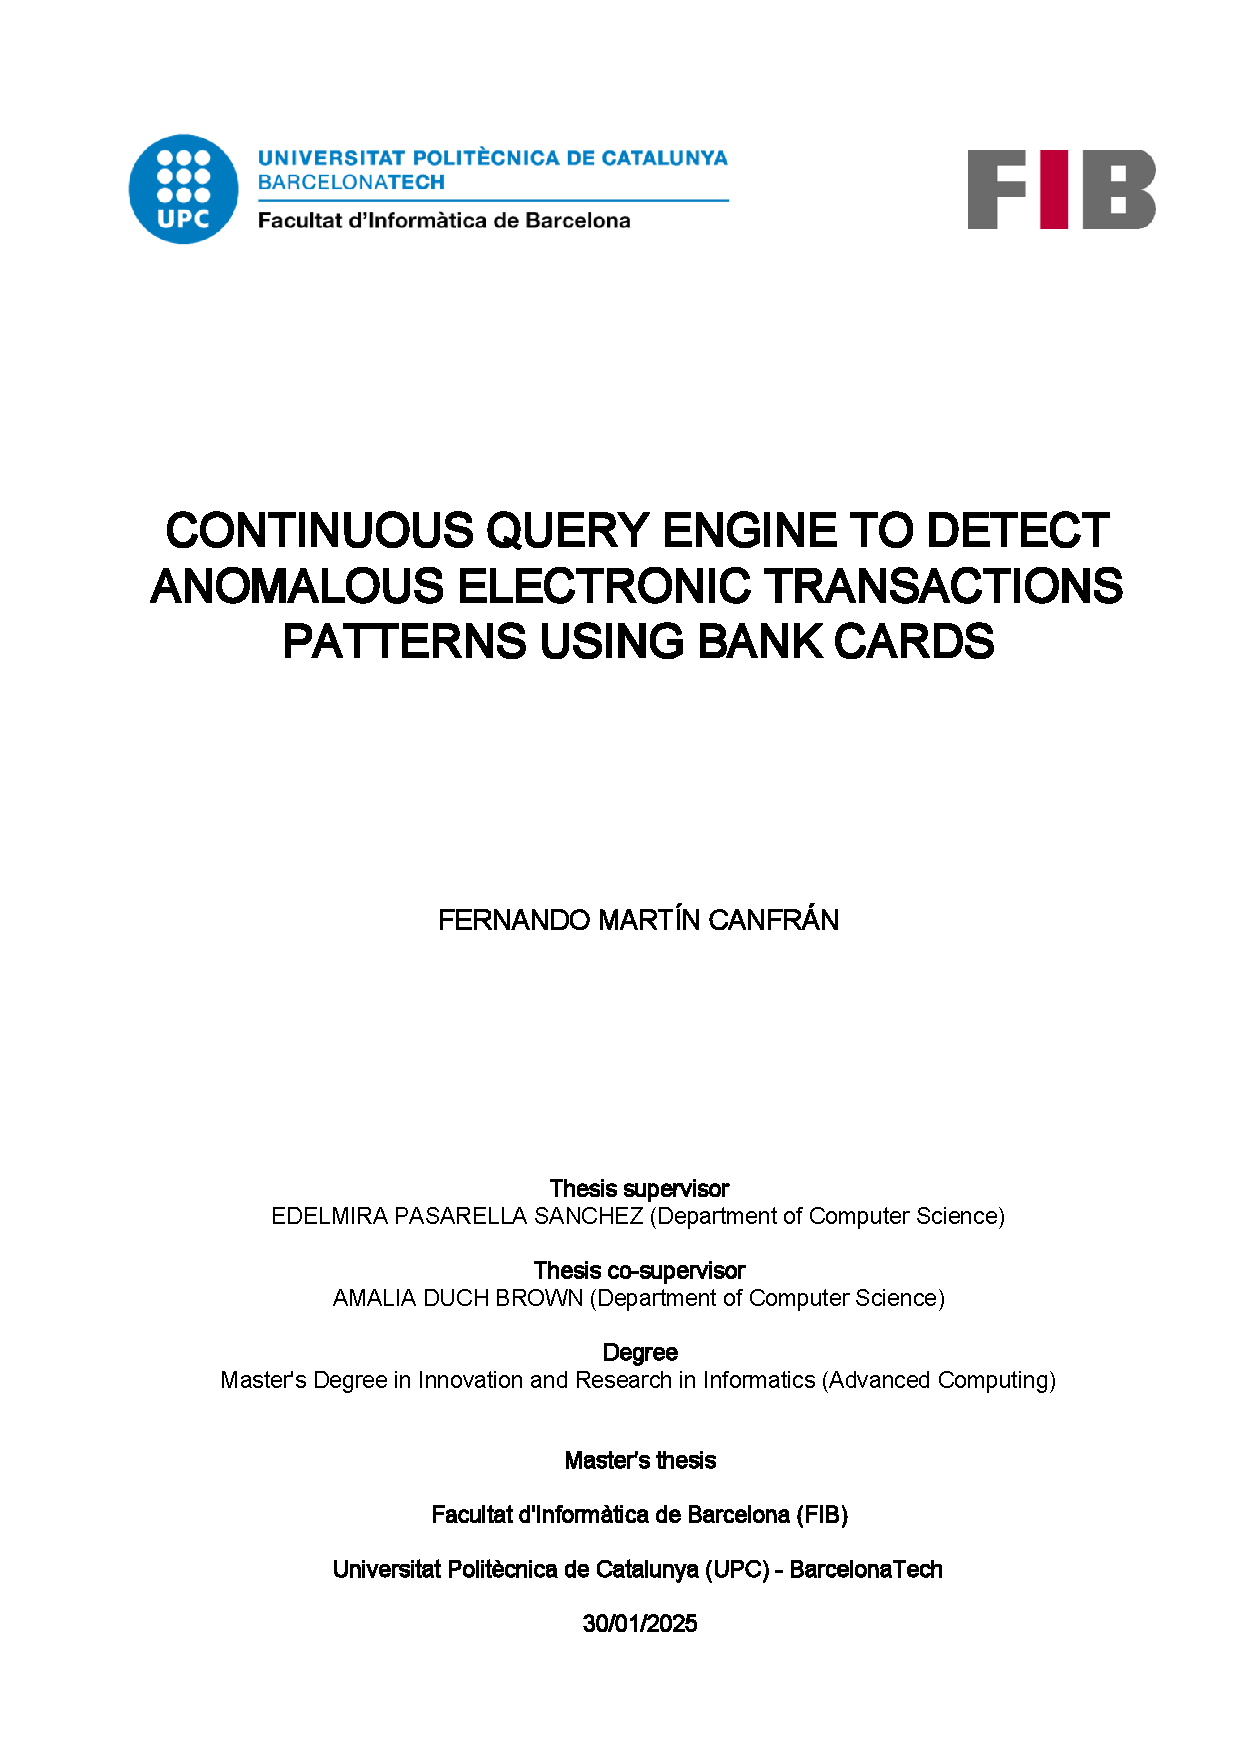
\includepdf{portada.pdf}

\begin{abstract}
Nowadays data are in motion, change continuously and are –potentially–
unbounded implying data sources that are also in constant evolution. From the  point of view of
data persistence, this reality breaks the usual paradigm of  dynamic although stable data sources. 
Besides, the number of applications to help critical decision making in real time is also rapidly increasing. 
These two scenarios raise the need of re-thinking both the data and the query models to fit these new requirements. 
So that, under these circumstances, it seems that a {\em continuously  evolving data graph} is a suitable data model to use and therefore to study and analyze.
Thus, in this work, we tackled the problem of querying continuously evolving data graphs in a specific context: 
the context of ATM\footnote{Automated teller machine} transactions, in particular anomalous ones. 
Under this context, evaluating continuous queries corresponds to recognizing patterns --usually associated with anomalous behaviors-- 
in the {\em volatile} (evolving) subgraph of ATM transactions. 
To do so, we propose an evaluation process based on the so called {\em dynamic pipeline
computational model}, a stream processing technique that facilitates  the emission of alerts as soon as anomalous patterns are identified. 
Stream based bank applications that monitor ATM transactions are direct beneficiaries of our proposal since they can continuously query data graphs 
to get “fresh” data as they are produced, avoiding the computational overhead of having to discard non-valid data, as current systems work.
\end{abstract} 

\keywords{continuous query evaluation, property graphs, dynamic pipeline approach, stream processing, ATM transactions}

\newpage

\section*{Acknowledgements}

I would like to express my gratitude to my teachers Edelmira Pasarella and Amalia Duch, whose guidance and support have been invaluable throughout this work. They have been always patient and have offered me great opportunities for my professional career that I will never forget. Thank you for everything.\\

In addition, I want to express my deep gratitude to Daniel Benedí, who has been a helping hand whenever I needed support throughout this long journey. Also to all the colleagues and friends from the master program.\\

I am also grateful to all the friends I have get to know during this chapter of my life in Barcelona. Without you, these two years would not have been the same. And, of course, to my friends from my hometown, Zaragoza, who have had the ability to stay by my side during these years, even if I have sometimes not spend much time with you.\\

Finally, and most importantly, to my family. Especially to my parents Jesús and Maria del Carmen, my sister María and to my grandmother Teresa, always in my memories. Thank you for everything. You are the best thing of my life.

\newpage

\tableofcontents

\newpage


\section{Introduction}
\label{sec:intro}
\iffalse
TODO:
\begin{itemize}
    \item Explicar el problema. Soluciones propuestas hasta ahora. Por qué no son suficientes. En qué consiste la nuestra.
    \item Definición general aplicación propuesta. Validez para PoS card fraud or internet frauds (CNP: Card Not Present frauds)... pero que hemos concretado en el caso de los ATM fraud.
    \fmc{Poner aquí contexto sobre los distintos tipos de fraude y sus estadísticas: referencia al informe SEPA ("Seventh report on card fraud typos")}
    \item Explicar cómo está organizado el documento.
\end{itemize}
\fi

As an example of critical decision making scenario in real time, we consider 
the problem of detecting anomalous usage patterns in bank card transactions. 
In particular, suppose a card is used to withdraw money in two different locations 
in an elapsed time interval that makes it impossible for the cardholder to physically 
move from one location to the other; let us suppose, for instance, 
that one ATM is in Barcelona and the other in Madrid and two transactions are made with 
the same card in less than an hour, one at each ATM. 
Note that we are not concerned here with the typical physical sabotage of ATMs to steal/clone data, 
but instead we are concerned with possible criminal situations beyond sabotage, 
such as cloned bank cards. While using a cloned bank card chances are that  
suspicious patterns like the one described above arise. 
This is exactly what our proposal aims to detect in order to prevent a crime from being carried out, 
thereby protecting the interests of both, the bank and the cardholder.\\

Although from a classical point of view databases consider data as persistent~\cite{abiteboul1995foundations}, 
nowadays this perspective is changing~\cite{babu2001continuous,zaniolo2012logical} as data is in motion, continuously changing 
and (possibly) unlimited. 
This is the case of ATM transactions. Indeed, transactions occur continuously and are not
(necessarily) bounded. 
In this setting, the fact that transactions should be somehow represented in banking 
databases makes us reconsider the meaning of their persistence in banking systems 
raising the following two questions: 
(i) What is the appropriate data model to deal with this kind of transactions? 
and (ii) What is the appropriate query model?\\

\noindent
Regarding the data model, the new nature of data requires a \emph{de facto} 
new database paradigm -\emph{continuously evolving  databases}- 
where data can be both \emph{stable} and \emph{volatile}. 
Even though evolving databases can be implemented according to any approach, 
graph databases seem especially well suited here {\cite{GDB-angles2008survey, GDB-kumar2015graph}. 
Indeed, the natural way to process evolving graphs as streams of edges gives insights 
on how to proceed in order to maintain dynamic graph databases.  
Hence, we consider that a suitable data model is a \emph{continuously evolving data graph}, 
a graph having persistent (\emph{stable}) as well as non persistent (\emph{volatile}) relations. 
Stable relations correspond to edges occurring in standard graph databases while volatile relations 
are edges arriving in data streams during a set time interval. 
Once this time interval is over, the relations are no longer valid so that there is no need to store 
them in the (stable) graph database. 
Volatile relations induce subgraphs that exist only while the relations are still valid. 
%
\noindent
In this work we tackled the problem of evaluating continuous queries corresponding to 
\emph{anomalous patterns} of ATM transactions against a continuously evolving graph database  
representing a bank database.\\

Without loss of generality we use  \emph{Property Graphs} (PG) 
\cite{PG-angles2017foundations, angles2018propertyGraphDatabaseModel} 
as the basic reference graph data model. 
As an example, Figure \ref{fig:constinuousPGa} depicts part of a schema of a 
PG database where stable relations correspond to the data that a bank 
typically gathers on its issued cards, ATMs (Automated Teller Machines) network, etc. 
Volatile relations model the interaction between cards and ATM entities.\\
%
\begin{figure*}[h]
    \centering
    \begin{subfigure}[b]{0.6\textwidth}
        \centering
        \includegraphics[width=0.85\textwidth]{images/schema.png}
        \caption{Part of a schema of a PG}
         \label{fig:constinuousPGa}
    \end{subfigure}%
     ~ 
    \begin{subfigure}[b]{0.4\textwidth}
        \centering
        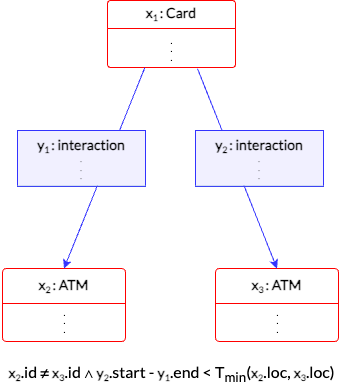
\includegraphics[width=0.85\textwidth]{images/graphPattern.png}
        \caption{Pattern of anomalous transactions}
        \label{fig:constinuousPGb}
    \end{subfigure}
    \caption{Part of a PG schema specifying volatile (\textsf{interaction} edges) and stable  (\textsf{issued\_by, owned\_by, interbank} edges) relations in an evolving ATM Network and a continuous query pattern.}
    \label{fig:constinuousPG}
\end{figure*}
%

\noindent
Concerning the query model, fixed queries evaluated over data streams are known 
as \emph{continuous queries} \cite{CQ-babu2001continuous,CQ-zaniolo2012logical}. 
Thus, instead of classical query evaluation processes we envision \emph{incremental/progressive} 
query evaluation processes. 
A query on a PG database can be seen as a PG graph pattern with 
constraints over some of its properties. 
Evaluating such a query consists on identifying if there is a 
subgraph of the database that matches 
the given pattern and satisfies its constraints. 
Figure \ref{fig:constinuousPGb} depicts the pattern 
corresponding to an anomalous situation in 
the volatile (PG) subgraph of the considered database. 
This is, a constrained graph pattern corresponding to a continuous query. 
An  anomalous pattern of ATM transactions must be identified in 
the volatile (PG) subgraph of the considered database.\\

The problem of progressively identifying and enumerating bitriangles 
(i.e. a specific graph pattern) 
in bipartite evolving graphs using the 
\emph{Dynamic Pipeline Approach} (DPA)\cite{DP-pasarella2024computational} 
have been successfully solved by Royo-Sales \cite{DP-bitriangles2021}.  
Let us observe that the problem of evaluating continuous queries over 
\emph{continuously evolving PGs} 
belongs to the same family of problems and hence we propose to address 
it using the same stream 
processing computational model.
%the {Dynamic Pipeline Approach}\cite{DP-pasarella2024computational}.  
Figure \ref{fig:theProblem} illustrates the model associated to the problem described at 
the beginning of this section. 
%
\begin{figure}[h]
         \centering
         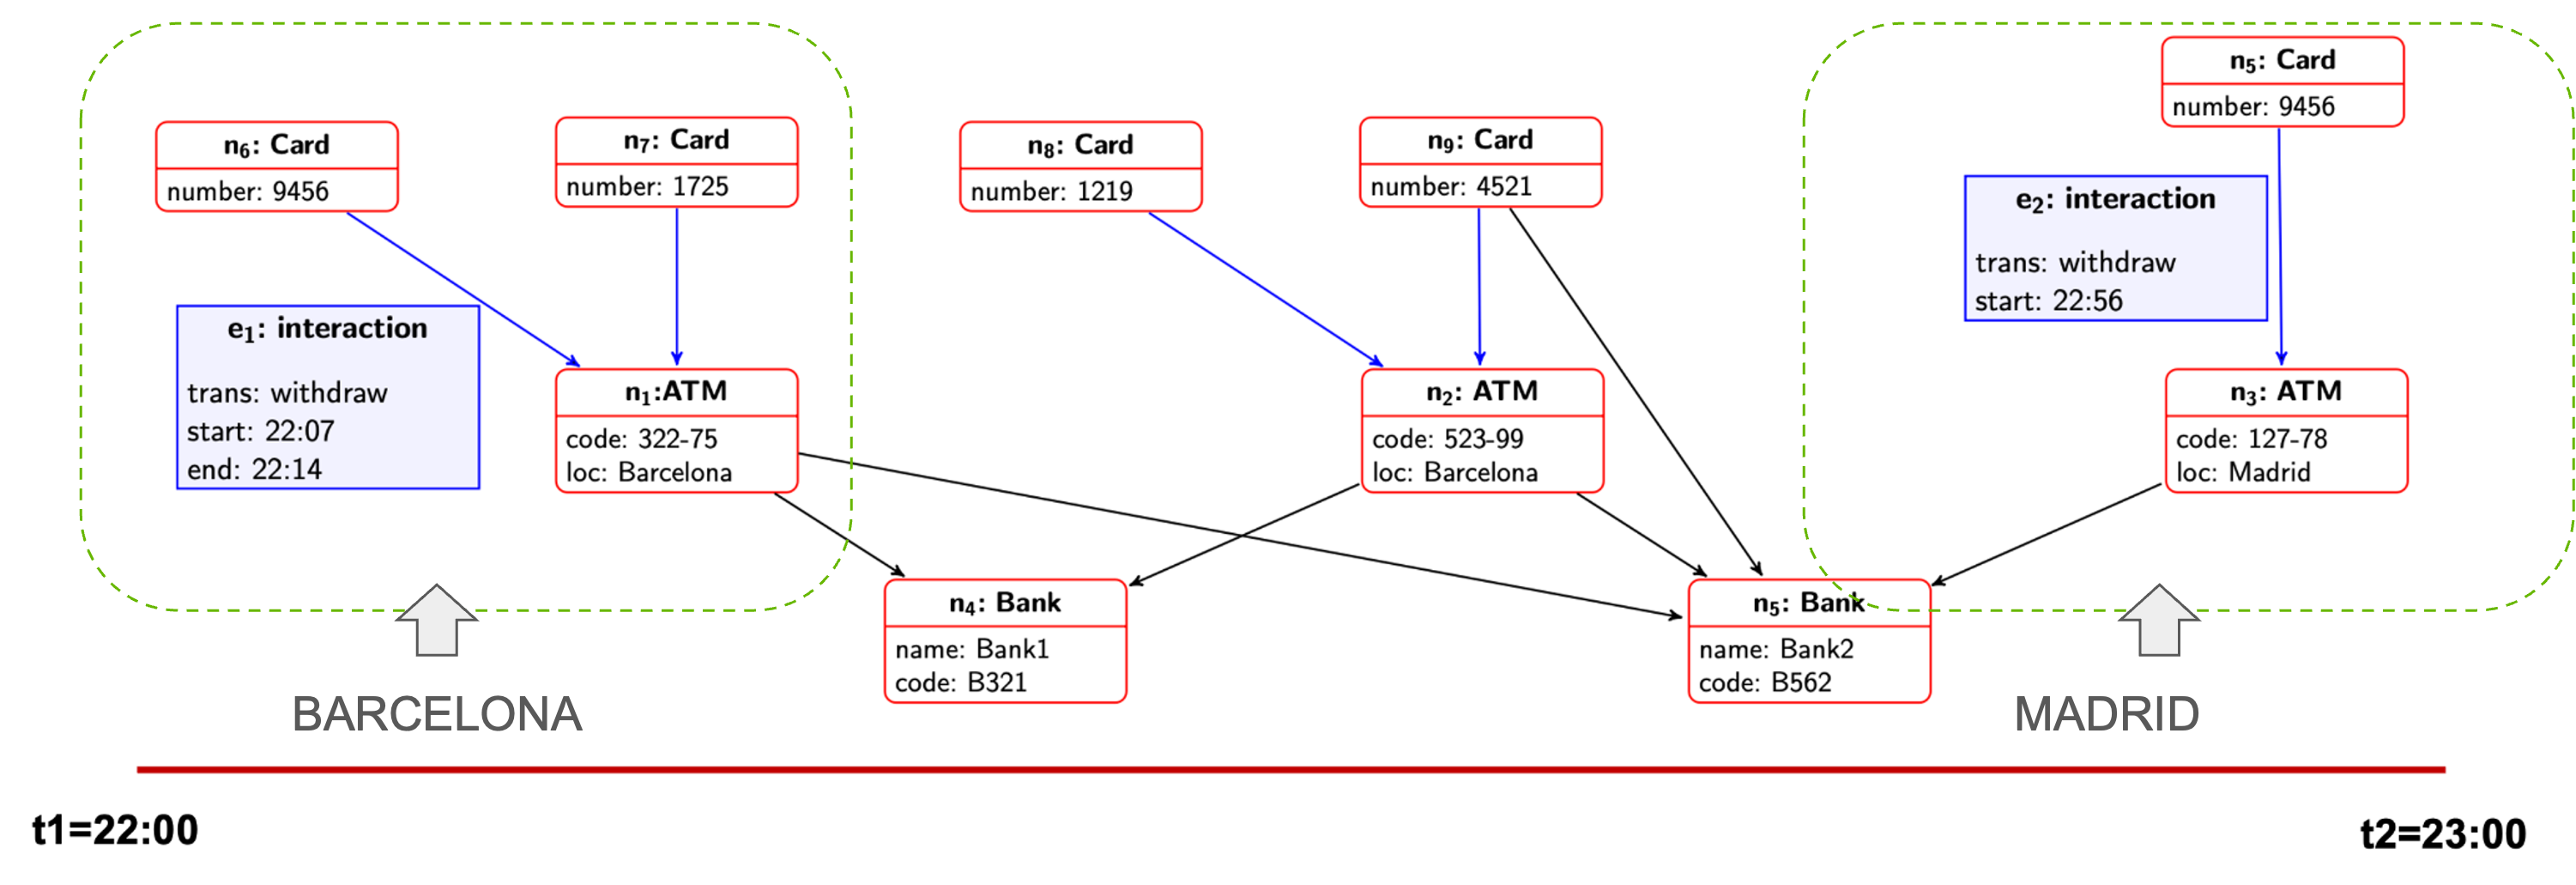
\includegraphics[width=0.85\textwidth]{images/theProblem.png}
         \caption{Example of the occurrence of anomalous ATM transactions in (a part of) 
         a continuously evolving PG over a time interval: the card \textsf{9456} is used twice at ATMs 
         in different cities, within one hour. 
         However, to get from one of the cities to the other and vice versa requires more 
         than one hour using any means of transport. 
         This example could represent a possible 
         crime pattern after a case of \emph{skimming} and \emph{cloning}.}
         \label{fig:theProblem}
\end{figure}
%
In addition to identify the query pattern, the constraint satisfaction 
over properties must be checked also.  
The evaluation process, done by a \emph{Continuous Query Engine} (CQE) 
is based on the dynamic pipeline computational 
model \cite{DP-pasarella2024computational} and  
emits  answers (alarms) as soon as anomalous patterns are identified. 
Moreover, in a real application,  
when required -as for further legal or auditing purposes- 
timestamped occurrences of volatile relations can  be kept in a log file. 
Figure \ref{fig:DP_ATM} depicts a basic architecture of a CQE.
%
\begin{figure}[h]
         \centering
         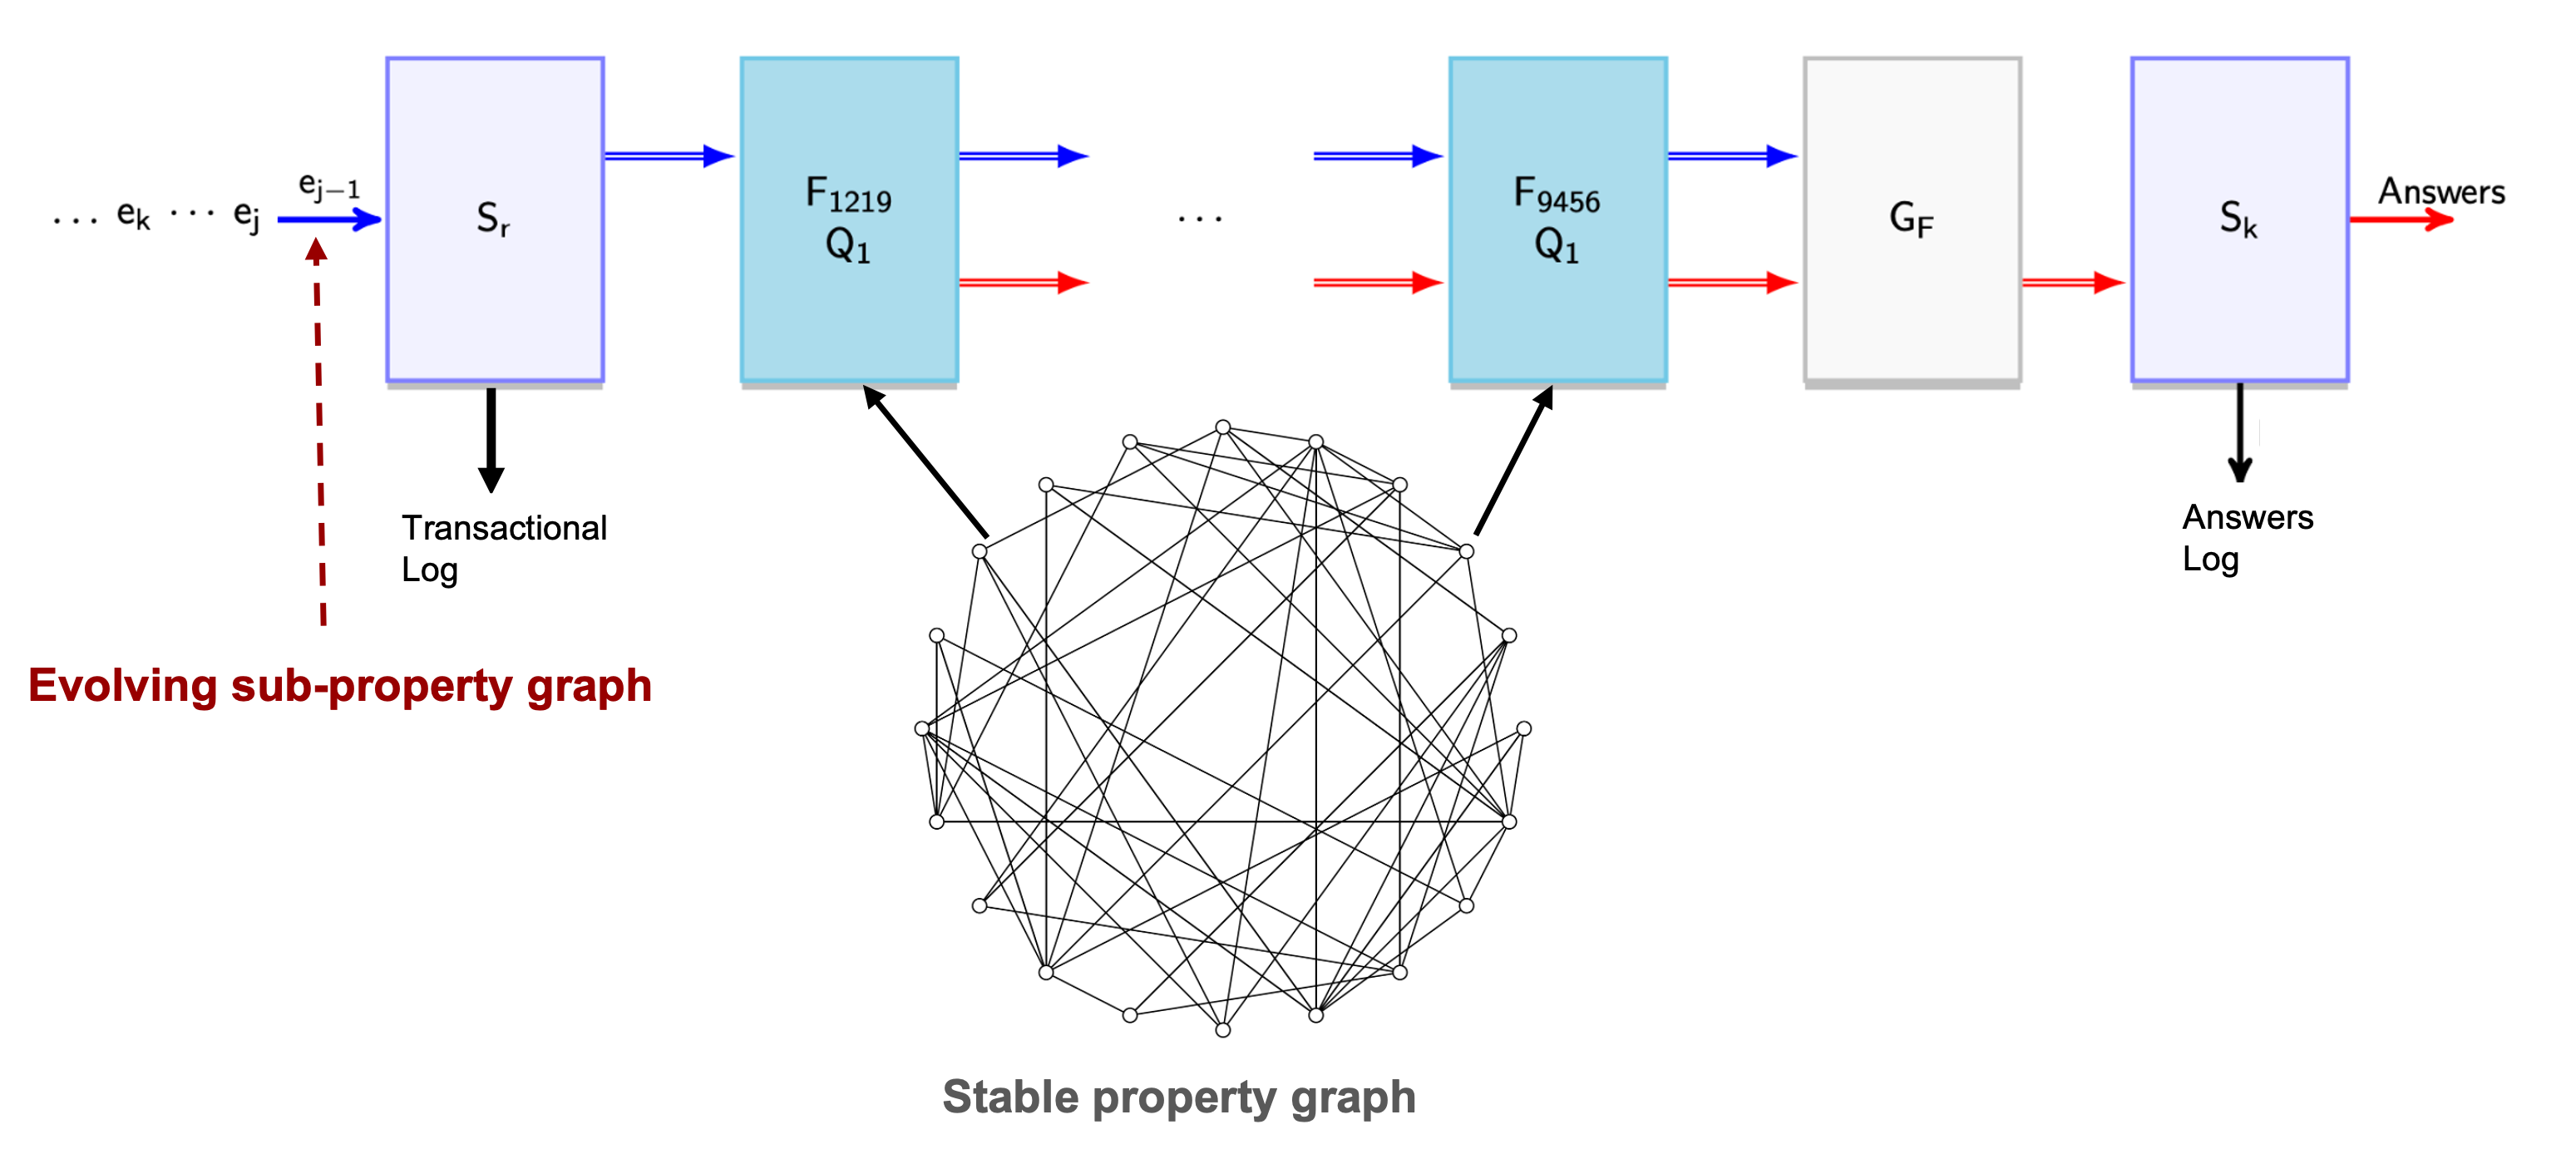
\includegraphics[width=0.7\textwidth]{images/architecture.png}
         \caption{Preliminary continuous query engine architecture for detecting anomalous 
         ATM transactions based on the dynamic pipeline computational model. 
         Considering the schema given in Figure \ref{fig:constinuousPGa}, 
         in this directed (multi) graph presentation of the $\mathsf{DP_{ATM}}$, 
         the arriving input data is a stream  $\mathsf{\langle \dots e_k\dots e_j \: e_{j-1}\rangle}$ 
         corresponding to \textsf{interactions} (volatile relations). 
         Boxes (vertices) represent \emph{stateful} processes called \emph{stages} 
         and internal arrows in the pipeline represent channels. 
         Blue channels carry interaction edges and red channels carry detected anomalies (answers).  
         $\mathsf{S_r}$ and $\mathsf{S_k}$ correspond to the \textsf{Source} and \textsf{Sink} 
         stages which receive input data and results, respectively. 
         \textsf{Filter} stages, $\mathsf{F_{N}}$, are parameterized with the value of the property 
         \textsf{number} ($\mathsf{N}$) of \textsf{Card} vertices. 
         The \textsf{Generator} stage, $\mathsf{G_F}$, is in charge of spawning new filters, 
         when required. The stable PG is a standard bank database (i.e. without volatile relations). 
         Transactional log and Answers log keep input interactions and answers, respectively.
         }
         \label{fig:DP_ATM}
\end{figure}

In order to test the practical suitability of our proposal, 
we have implemented it in the \texttt{Go} programming 
language since this language easily provides connection 
to existing implementations of Neo4j graph databases 
such as the one we use in this work, in addition to providing the necessary 
tools to exploit the parallel 
and distributed properties of the DPA with which we represent our proposal.
Additionally, in order to experiment with the performance of our model, 
we provide a program capable of generating synthetic datasets useful 
to simulate bank graph databases including several parameters such as the users, 
their card holders, their ATMs geographically distributed, 
the stream of transactions, etc.\cite{ATM-DP-github}
We assessed our model with two different bank sizes considering standard metrics as well as specific ones \cite{exps-diefficiency} for measuring continuous behavior  
and we could observe that (compared to a sequentially implemented system) 
the proposal using the DPA performs clearly better, 
providing almost immediate responses to the tested queries. 
Additionally, as opposed to artificial intelligence approaches \cite{ahmed2016survey,} to predict frauds, 
ours provides 100\% of effectiveness detecting fraud patterns. 
This is, there is no place to consider false alarms (false positive recognition of pattern)  
or ignore alarms due to non-recognition of patterns (false negative) since,  
in presence of the studied fraud pattern, the CQE will recognize it. Partial results of this work were reported and presented in the Alberto Mendelzon Workshop 2024 \cite{martincanfran2024AMW}. 
We can summarize the contributions of this work as follows.

\paragraph{Contributions.}
\begin{itemize}
\item A general technique for addressing the problem of continuous 
query evaluation against an evolving graph database by decomposing 
the data graph into \emph{volatile} and \emph{stable} well defined subgraphs, 
using a stream processing approach.  
Among the advantages of using the dynamic pipeline computational 
model are its parallel/concurrent nature and its suitability for 
developing real-time systems that emit results as they are computed, 
in a progressive way. 
\item A characterization of some possible fraud graph patterns. Even non-exhaustive, to our knowledge, it is a first specification of what must be consider a fraud pattern in terms of (continuous) graph databases. This characterization is useful not only when considering ATM transactions but, in general,  for any bank cards online transactions.
\item A continuous query engine  to detect abnormal or suspicious ATM transactions. 
To our knowledge, most of the work addressing this topic provide a delayed 
detection based on predictions given by ML systems. 
Also, it is frequent the classical treatment of the problem by consulting 
log files because of the complaint of customers when detecting by 
themselves some weird  movement in their accounts. 
This involves annoying processes for customers in order to have their money back. 
The idea is that, in presence of some weird  finding in an ATM transaction, 
banks have a tool able to either ask card holders for authorizations 
or to take any action preventing other fraud at real-time.
\item Given the sensitive nature of banking data and transactions, 
there are no repositories that offer this type of datasets for empirical studies. 
In this work, we have created an open synthetic repository for this purpose. 
\end{itemize}

The rest of this work is organized as follows. 
In Section \ref{sec:related_work}, we describe the related existing work while, 
in Section \ref{sec:prelim}, we give the required preliminaries to follow the whole work 
regarding graph databases, graph fraud patterns, the dynamic pipeline paradigm and
the metrics used to evaluate the features of our proposal.
In Section \ref{sec:proposal}, we describe the details of our proposal by 
defining anomalous patterns of transactions, how to 
model and implement the continuous query engine, the used data model and query model 
as well as the architecture of the continuous query engine.
Section \ref{sec:CQE-DPATM} is devoted to the continuous query engine, the 
$\mathsf{DP_{ATM}}$. The experiments are described in Section \ref{sec:experiments} where 
the different evaluation scenarios, the experimental settings, the datasets and 
the stream configurations are considered. The experimental results are analyzed in Section \ref{sec:results}
and in Section \ref{sec:concl} we give some conclusions and proposals for further work.


\section{Related Work}

\textcolor{gray}{TODO: 
\begin{itemize}
    \item Explicar toda la bibliografía relevante con pros y contras de cada propuesta.
\end{itemize}
}
\section{Preliminaries}
\subsection{Graph databases}
%%

References:
\begin{itemize}
    \item PG: \cite{PG-angles2017foundations, PG-angles2018propertyGraphDatabaseModel, PG-Graphs-at-a-time-GraphQL-QueryLanguage, PG-exampleUsageSimeonovski}
    \item Graph Databases: \textcolor{blue}{\cite{GDB-angles2008survey, GDB-kumar2015graph}}
\end{itemize}
\subsection{Graph fraud patterns}
xxxxx
\fmc{Aqui ponemos referencias / describimos los fraudes bancarios que existen... informe SEPA? - o solo en la introducción?}
%%
\subsubsection*{Graph Database Model: Property Graph}

Informally, a property graph is a directed labeled multigraph with the special characteristic that each node or edge could maintain a set (possibly empty) of property-value pairs \cite{angles2018propertyGraphDatabaseModel}. In this graph, a node represents an entity, an edge a relationship between entities, and a property represents a specific feature of an entity or relationship. 
A more formally  (as defined in \cite{PG-exampleUsageSimeonovski}):

\begin{definition}
A property graph $G=(V,E, \lambda, \mu)$ is a directed labeled multigraph where $V$ is a set of nodes, $E \subseteq (V \times V)$ is a set of edges, $\lambda: V \cup E \rightarrow \Sigma$ is a function that labels nodes and edges with symbols of the alphabet $\Sigma$, and $\mu: (V \cup E) \times K \rightarrow S$ is a function that associates key-value properties, e.g., $(k,s)$ where $k \in K$ is the key and $s \in S$ is the string value, to nodes and edges.  
\end{definition}

\ad{Aqui estaría bien un ejemplo pequeño, dos nodos con un arco entre ellos y varias posibles propiedades, para que quede bien claro lo que es.}

\ad{añadir algo como lo siguiente: In the Graph Database community there several popular models of property graphs. Maybe the two most famous and used ones are \ldots 
los dos màs famosos con cita a algun sitio que diga que son los más famosos}

\ad{Muy importante: antes de explicar detalles específicos de Neo4j hay que explicar todo lo que es genérico de los property graphs y ponerlo aquí, fuera de la subsección de Neo4j}

\subsubsection*{Graph Database System: Neo4j}

Graph Databases: \textcolor{blue}{\cite{GDB-angles2008survey, GDB-kumar2015graph}}
% TODO: 
% - Poner definición 
% - Decir cuál elegimos: Neo4j y por qué

A graph database system is a system specifically designed for managing graph-like data following the basic principles of databases systems. 

%%
%%
\subsection{Dynamic Pipeline Paradigm}\label{DPP}

\textcolor{gray}{To explain:
\begin{itemize}
    \item PP (Pipeline Parallelism) computational model. The definition
    \item DP stages y un poco que hace cada stage
    \item Problemas que ya se han resuelto con este paradigma. Referenciar.
\end{itemize}
}

\fmc{Definición - Tomada de TFM Dani y J Pablo... completar mas?}

\ad{Yo creo que puedes citar ambas tesis y también el paper de Edelmira y explicar lo que es pero no hace falta que entres en demasiado detalle general, eso sí, los detalles de cómo lo usas para lo tuyo sí deben estar completos.}
In the context of Stream Processing, many data driven frameworks have emerged to address the management of continuous data streams. Dynamic data processing, characterized by the adaptive and responsive manipulation of large datasets in real time, and incremental generation of results, represent pivotal approaches.\\

One such model for Stream Processing is the Dynamic Pipeline Paradigm ($\mathsf{DPP}$) \cite{DP-pasarella2024computational}. The $\mathsf{DPP}$ is a PP (Pipeline Parallelism) data driven computational model that operates as a one-dimensional, unidirectional chain of stages connected by means of data channels. Essentially, the paradigm establishes a computational model rooted in the deployment of a linear pipeline consisting of a chain of stages structure called Dynamic Pipeline ($\mathsf{DP}$). It stretches and
shrinks depending on the spawning and the lifetime of its stages, respectively. Stages are processes that execute tasks concurrently/in-parallel.\\

\begin{figure}[H]
  \centering
  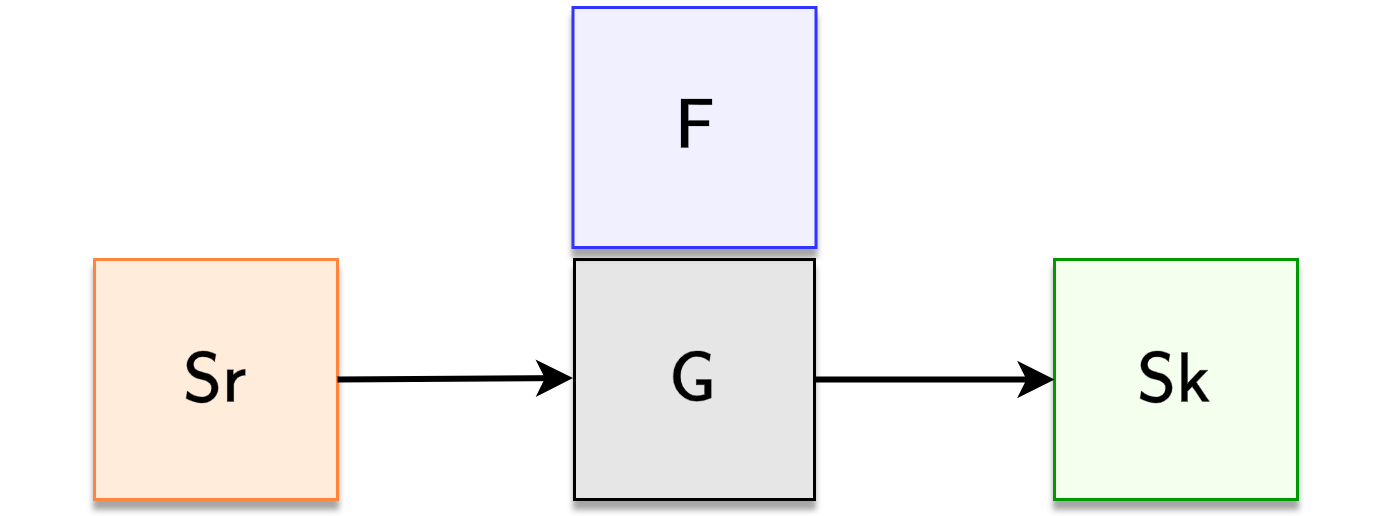
\includegraphics[scale = 0.7]{images/3-Engine/DP-Stages-1.png}
  \caption{Initial configuration of a Dynamic Pipeline. An initial $\mathsf{DP}$ consists of three stages: \emph{Source} ($\mathsf{Sr}$), \emph{Generator} ($\mathsf{G}$) and \emph{Sink} ($\mathsf{Sk}$). Above the  \emph{Generator} ($\mathsf{G}$) the \emph{Filter} ($\mathsf{F}$) parameter. The stages are connected through its channels, represented with the black right arrows.}
  \label{img:DP-Stages-1}
\end{figure}

These stages can be of four different types: \emph{Source} ($\mathsf{Sr}$), \emph{Filter} ($\mathsf{F}$), \emph{Generator} ($\mathsf{G}$) and \emph{Sink} ($\mathsf{Sk}$). \emph{Source} stage are the responsible of obtaining the input data stream and feeding it into the pipeline. \emph{Filter} stages maintain a state and process the incoming data processing it accordingly and/or passing it again to the pipeline. \emph{Generator} stage is in charge of spawning new \emph{Filter} stages when needed based on the incoming data, providing the \textit{dynamic} behavior to the model. Finally, \emph{Sink} stage receives the results, processing and acting on them as needed.
Figure \ref{img:DP-Stages-1} represents the initial configuration of a $\mathsf{DP}$ and Figure \ref{img:DP-Stages-2} depicts the stages of the $\mathsf{DP}$ after a possible evolution, where the \emph{Generator} has created two \emph{Filter} stage instances.\\

\begin{figure}[H]
  \centering
  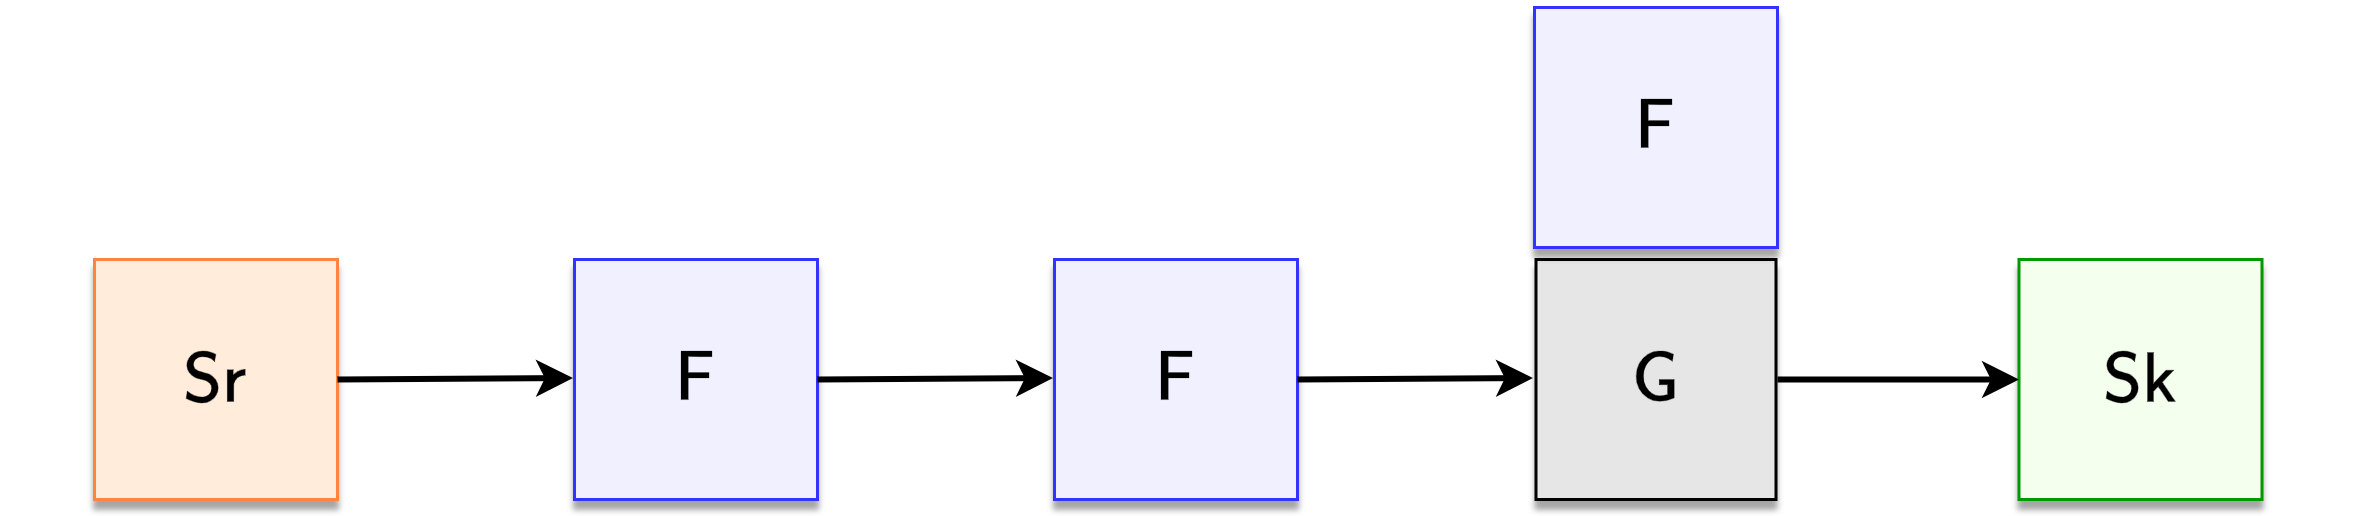
\includegraphics[scale = 0.7]{images/3-Engine/DP-Stages-2.png}
  \caption{Evolution of a $\mathsf{DP}$. After the creation of two \emph{Filter} $\mathsf{F}$ stage instances of the \emph{Filter} parameter (above the $\mathsf{G}$ stage) by the \emph{Generator} $\mathsf{G}$ stage.}
  \label{img:DP-Stages-2}
\end{figure}

The $\mathsf{DPP}$ has been used to model many different problems. In \cite{DP-bitriangles2021} they successfully solved the problem of progressively identify and enumerate bitriangles (i.e. a specific graph pattern) in bipartite evolving graphs. In \cite{DP-Lugosi_Enes_2019} $\mathsf{DPP}$ is used to model the problem of multidimensional range queries, that is, selection queries on objects in a k-dimensional space. Finally, in \cite{DP-Benedi_Garcia_2024} they solve the problem of computing and maintaining the minimum spanning tree of dynamic graphs.\\

In our case, we envision the architecture of our continuous query engine to detect anomalous ATM transactions under the $\mathsf{DPP}$, where the continuous input data stream is the stream of the bank ATM transactions, and we track the activity of a Card on a certain \emph{Filter} stage. Details on how the modeling of our problem with the $\mathsf{DPP}$ can be found in \ref{ContinuousQueryEngine}.
%%
%%
\subsection{Diefficiency metrics}

\fmc{Las tengo en \ref{exps:evaluation-metrics}, aquí hacer referencia y citar las de diefficiency del artículo y la herramienta utilizada, luego ya en el apartado de Experiments ponerlas todas (+ las adicionales añadidas, como interactions/s o el response time)}







\begin{frame}{Proposal}

\begin{enumerate}
    \item Data Model
    \vspace{1em}
    \item Definition of Anomalous Patterns of Transactions
    \vspace{1em}
    \item Query Model
    \vspace{1em}
    \item Continuous Query Engine - $\mathsf{DP_{ATM}}$
    \vspace{1em}
    \item Architecture
\end{enumerate}
\end{frame}

\begin{frame}{Proposal: Data Model}

\begin{itemize}
\item Nature of our data: ATM transactions on a bank system.
\begin{itemize}
    \vspace{0.5em}
    \item[$\Rightarrow$] \textcolor{red}{Dynamic} data sources. Transactions occur continuously.
\end{itemize}
\vspace{2em}
\pause
\item \textbf{\emph{Continuously evolving database}} - data can be stable and volatile.
\begin{itemize}
    \vspace{0.5em}
    \item[$\Rightarrow$] Graph Data Model: Property Graph (PG).
    \vspace{1em}
    \item[$\Rightarrow$] Graph Database System: Neo4j (based on PG).
\end{itemize}
\end{itemize}
\end{frame}

\begin{frame}{Proposal: Data Model}
    \begin{columns}
        % First Column (Stable PG)
        \column{0.5\textwidth}
        \begin{center}
            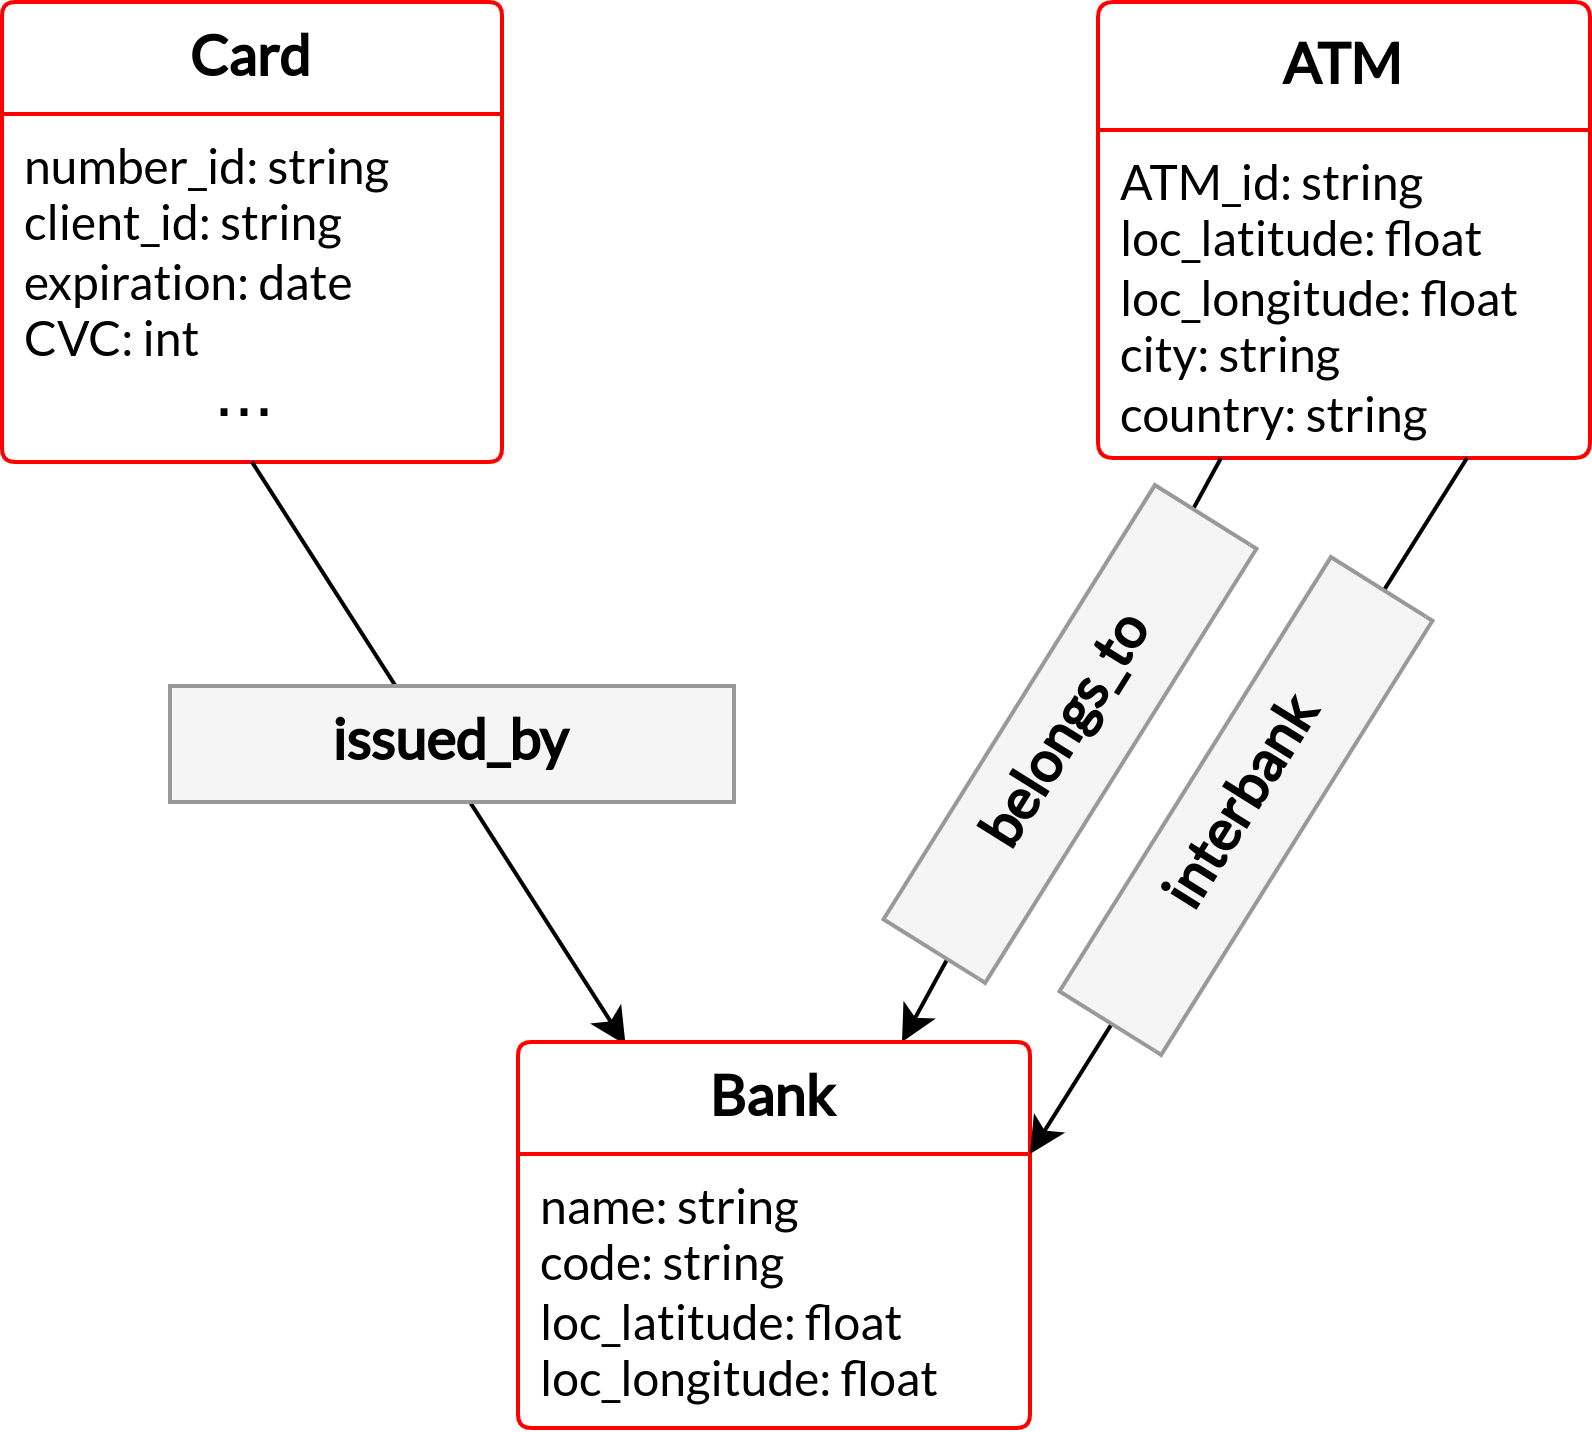
\includegraphics[width=1.0\textwidth]{figures/stable-presentacion-1.png}  
        \end{center}

        % Second Column (Volatile PG)
        \column{0.5\textwidth}
        \begin{center} 
            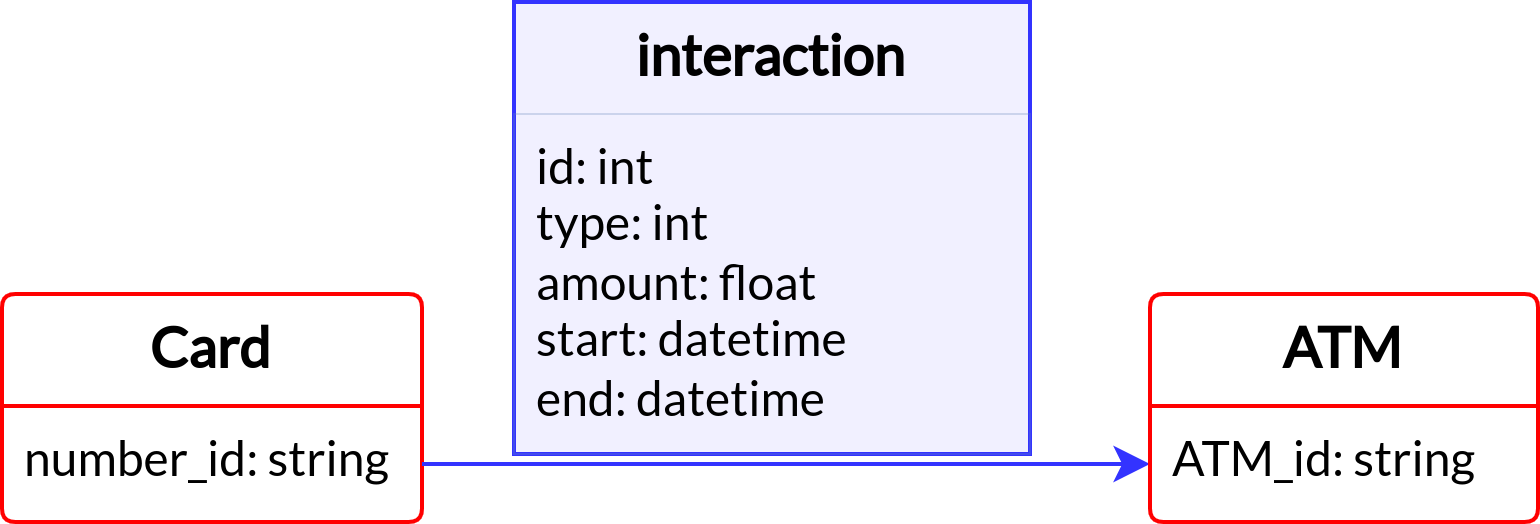
\includegraphics[width=1.0\textwidth]{figures/volatile-presentacion-1.png}
        \end{center}
    \end{columns}
    \vspace{0.6em}
    \begin{columns}
        \column{0.5\textwidth}
        \hspace{4.7em}\textcolor{blue}{Stable PG} \\Central bank database 
        {\small(\emph{persistent relations of standard graph dbs).}}
        \column{0.5\textwidth}
        \hspace{4.7em}
        \textcolor{blue}{Volatile PG} \\
        \vspace{0.3em}
        Transactions 
        {\small(\emph{non-persistent relations. Edges in the data stream).\\
        \textbf{Induced subgraphs in the \DPATM.}}}
    \end{columns}
    
\end{frame}


\begin{comment}
\begin{frame}{Proposal: Data Model}

\only<1>{
\begin{itemize}
    \item [$\Rightarrow$] Stable PG
    \begin{itemize}
    \item Models the data a bank typically gathers on cards, ATMs...
    \end{itemize}
\end{itemize}
}

\only<2>{
\begin{itemize}
    \item [$\Rightarrow$] Volatile PG
    \vspace{0.2em}
    \begin{itemize}
        \item Volatile relations (transactions) are the \textcolor{red}{edges arriving in data streams} during a set time interval. 
        \item \textcolor{red}{Induce subgraphs} that exist only while the relations are still valid.
    \end{itemize}
\end{itemize}
}

\begin{figure}
    \centering
    \only<1>{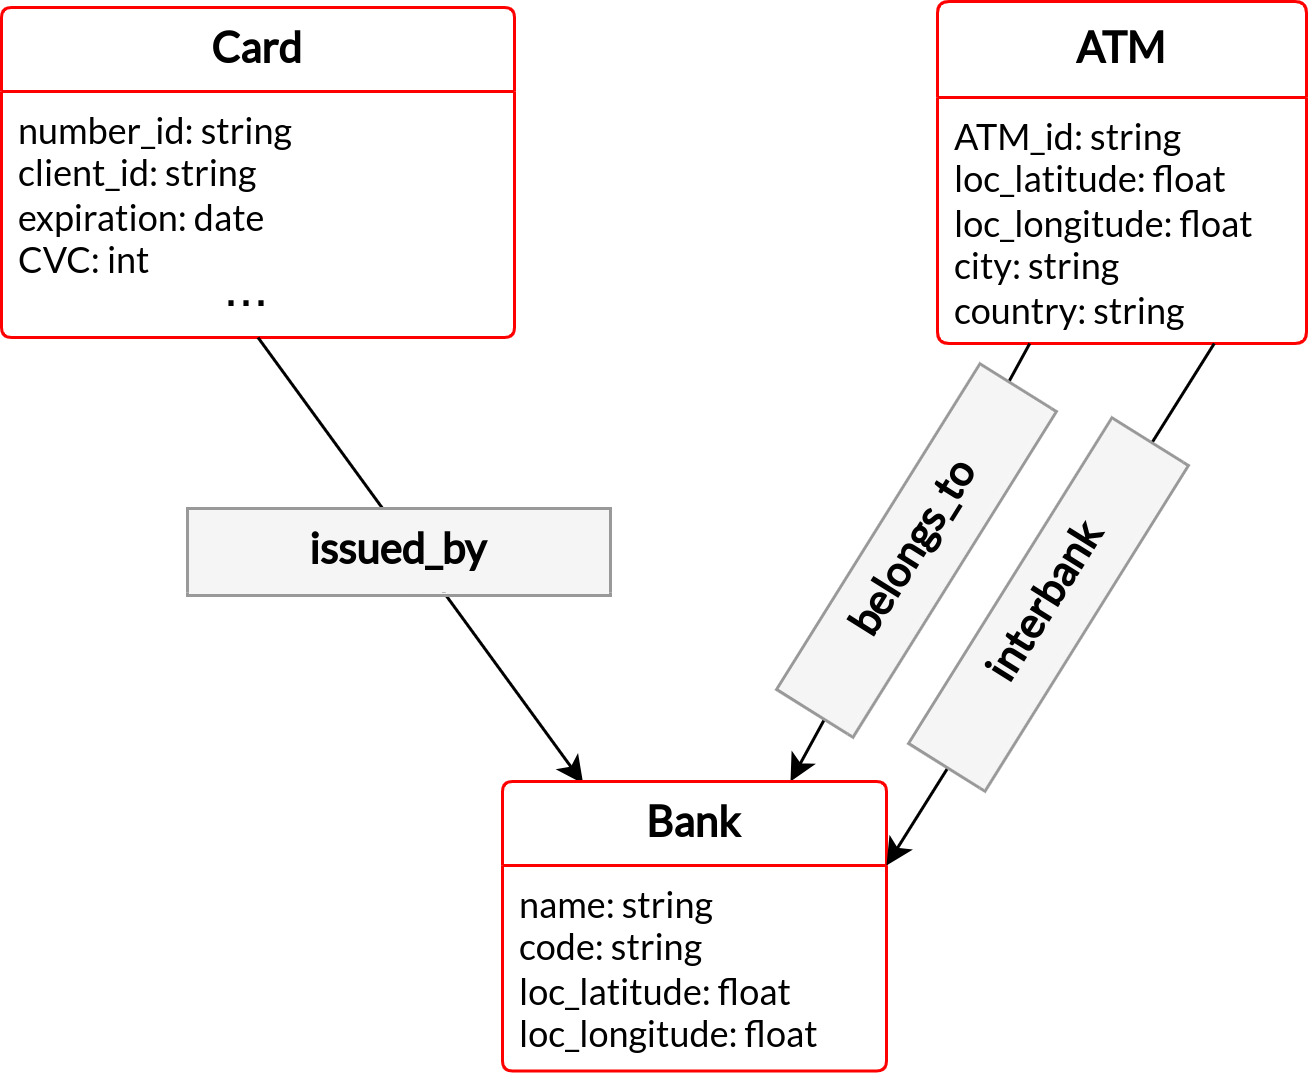
\includegraphics[width=0.65\textwidth]{figures/stable-presentacion.png}}
    \only<2>{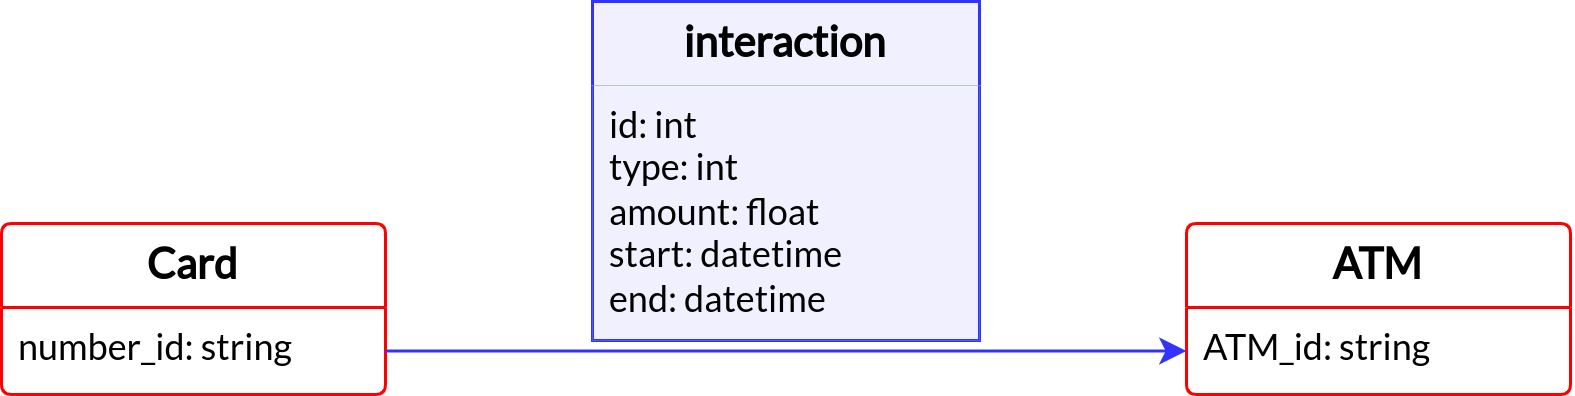
\includegraphics[width=0.8\textwidth]{images/1-DataModel/schema-volatile.png}}
\end{figure}

\end{frame}
\end{comment}


\begin{comment}
\begin{frame}{The data model: Stable PG}

\begin{figure}
    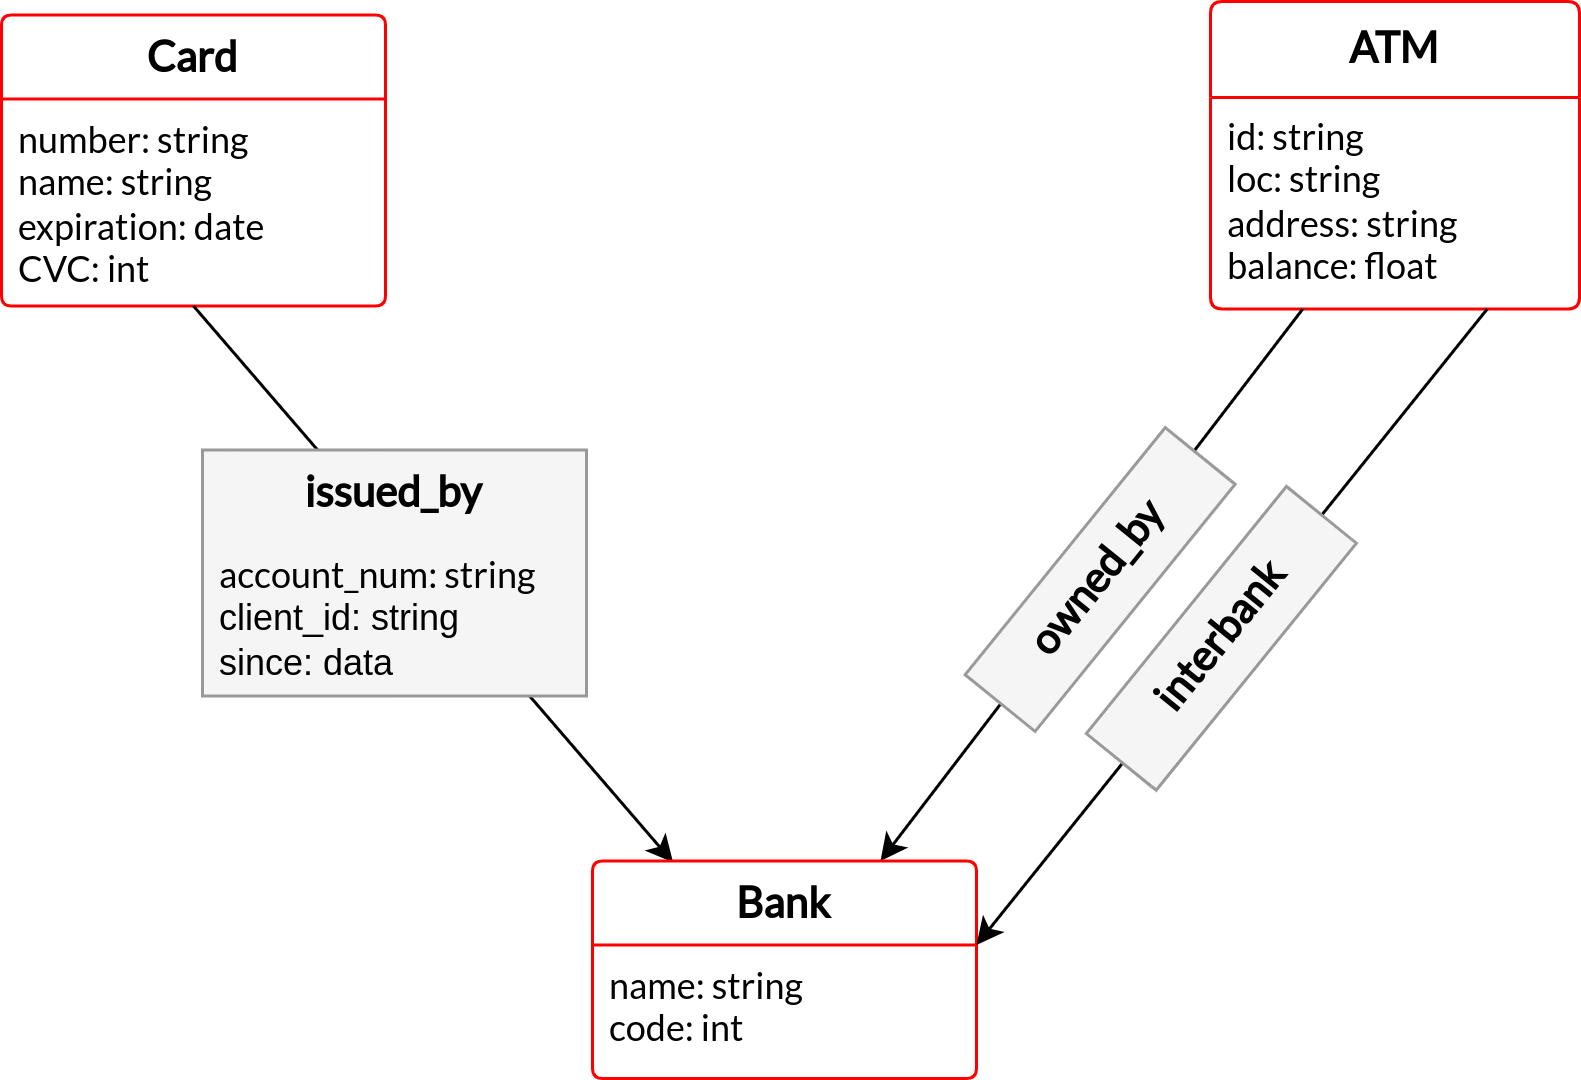
\includegraphics[width=0.8\textwidth]{figures/stable.png}
\end{figure}

\begin{itemize}
    \item Models the data a bank typically gathers on cards, ATMs...
\end{itemize}
\end{frame}

\begin{frame}{The data model}
\begin{figure}
    \includegraphics[width=0.9\textwidth]{figures/schema.png}
\end{figure}
\end{frame}

\begin{frame}{The data model: Volatile PG}

\begin{figure}
    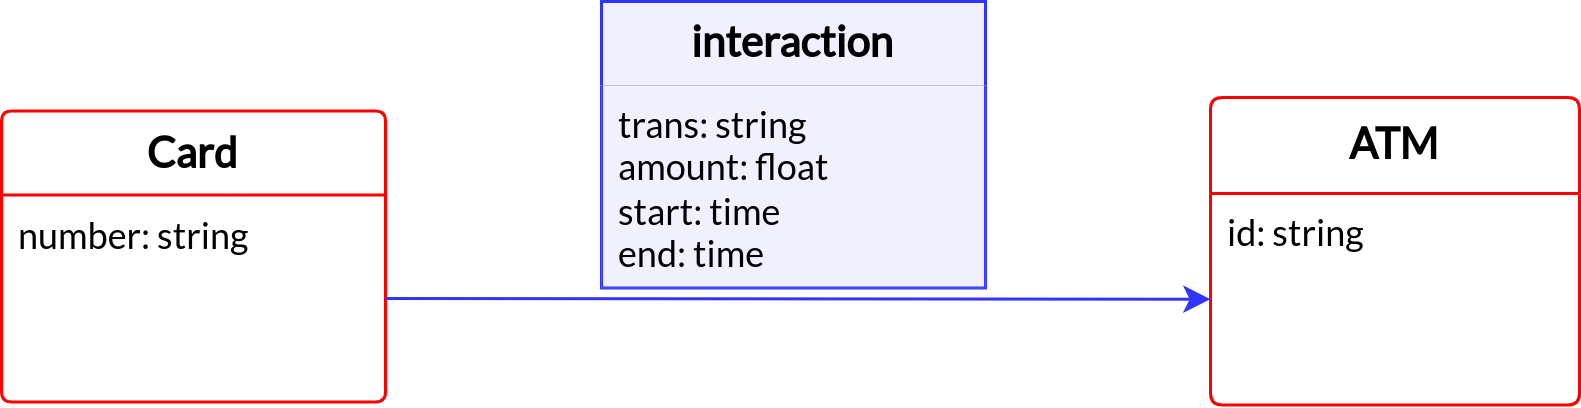
\includegraphics[width=0.9\textwidth]{figures/volatile.png}
\end{figure}

\begin{itemize}
    \item Models the interactions between cards and ATM entities.
    \item Volatile relations (transactions) are the edges arriving in data streams during a set time interval. 
    \item Induce subgraphs that exist only while the relations are still valid.
    \item Minimal information (only identifiers) on its nodes. 
\end{itemize}

\end{frame}

\begin{frame}{The data model: Volatile subgraph}
\textbf{Note}: Creation of 2 edges per transaction - the \emph{opening} edge and the \emph{closing} edge.
\textbf{Important} for some anomalous query patterns, to detect them before they are completely committed. 

\begin{figure}
    \centering
    \only<1>{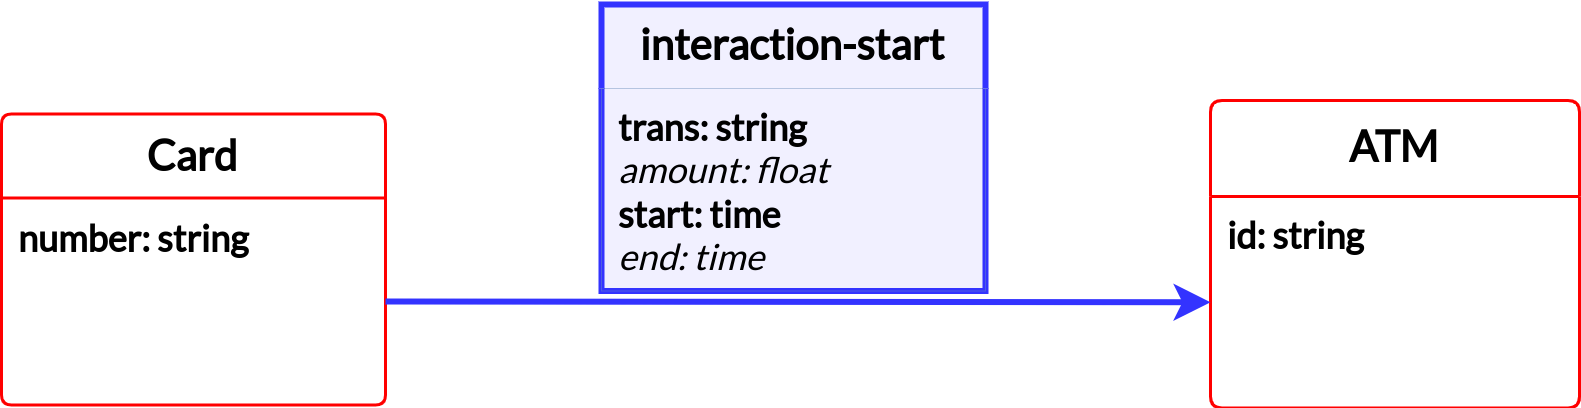
\includegraphics[width=\textwidth]{figures/2-edges-tx-start.png}}
    \only<2>{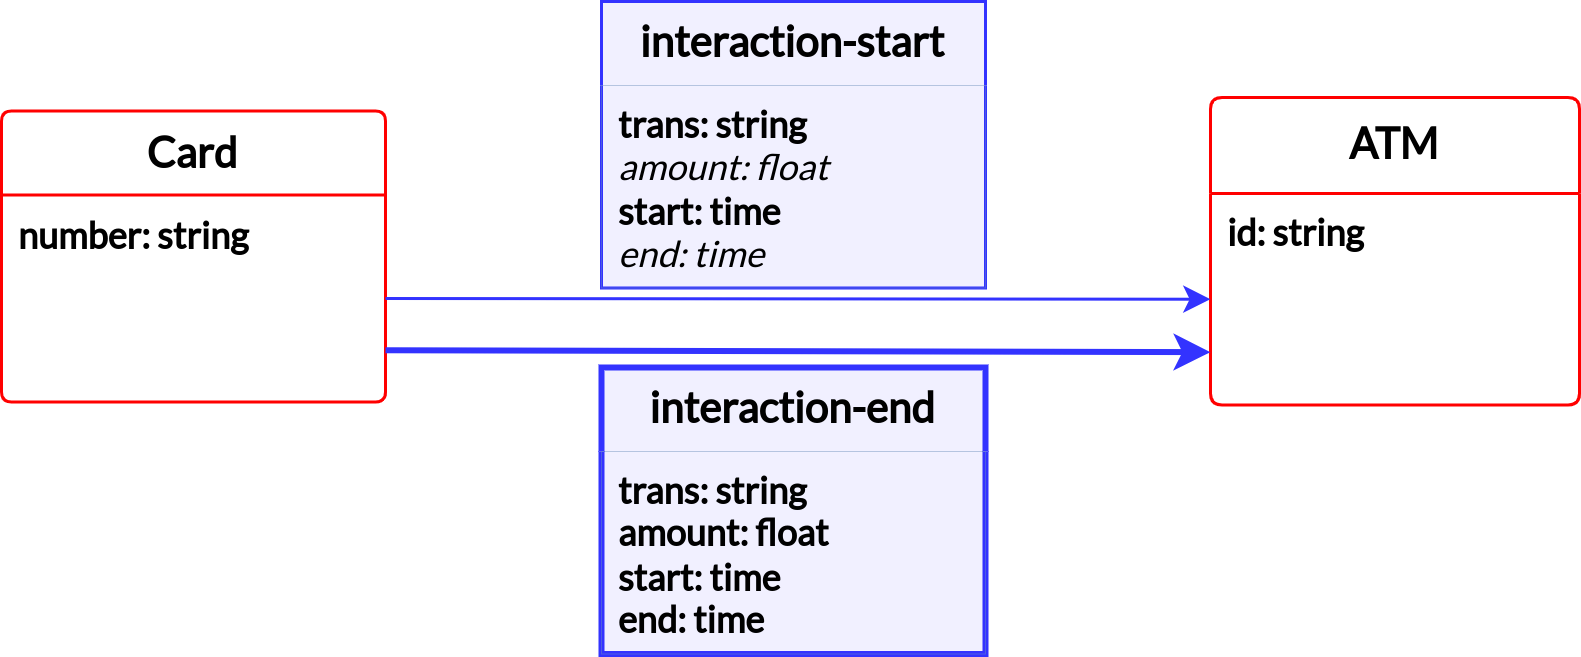
\includegraphics[width=\textwidth]{figures/2-edges-tx-end.png}}
    \caption{\only<1>{Opening edge}\only<2>{Closing edge}}
\end{figure}

\end{frame}

\end{comment}

\begin{frame}{Proposal: Definition of Anomalous Patterns of Transactions}
\begin{figure}
    \hspace*{-0.6cm}
    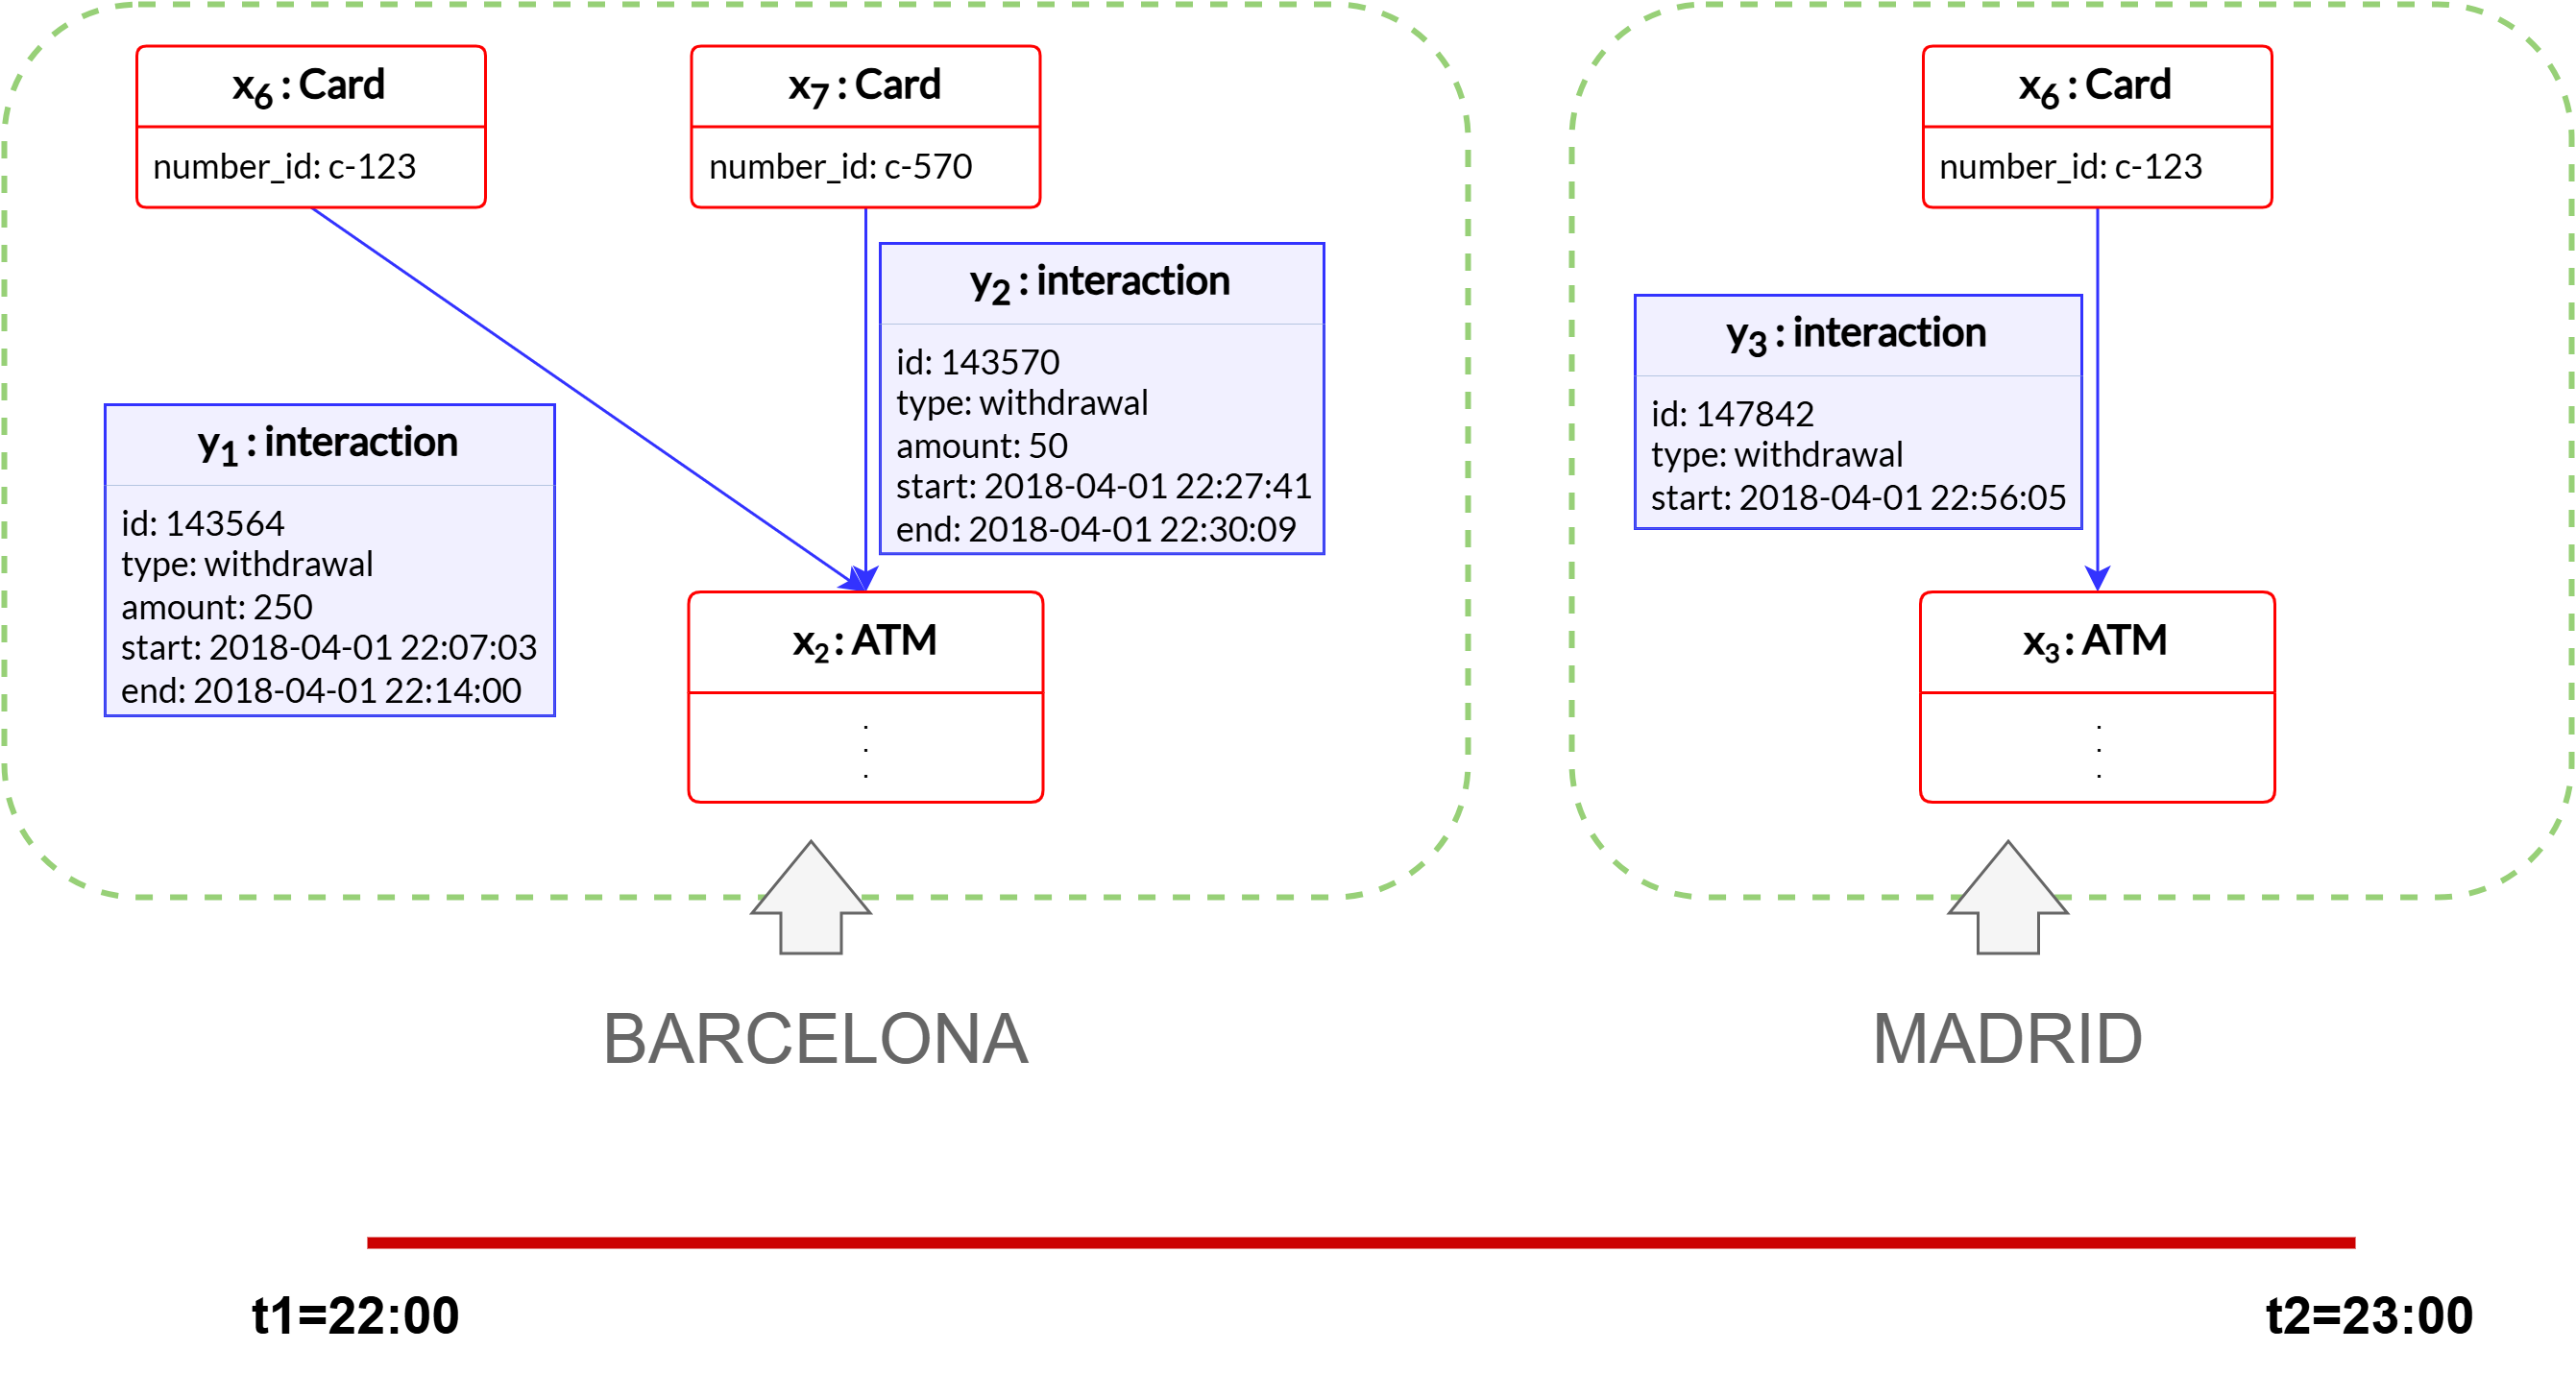
\includegraphics[width=1.10\textwidth]{images/2-QueryModel/FP1-Example.png}
    \caption*{Card cloning characterization - an example}
\end{figure}
\end{frame}

\begin{frame}{Proposal: Definition of Anomalous Patterns of Transactions}
\begin{itemize}
    \item Continuous queries are characterized as (constrained) \textbf{graph patterns}
\end{itemize}   
\begin{columns}
      % primera columna
      \begin{column}{0.3\textwidth}    
        \begin{figure}
            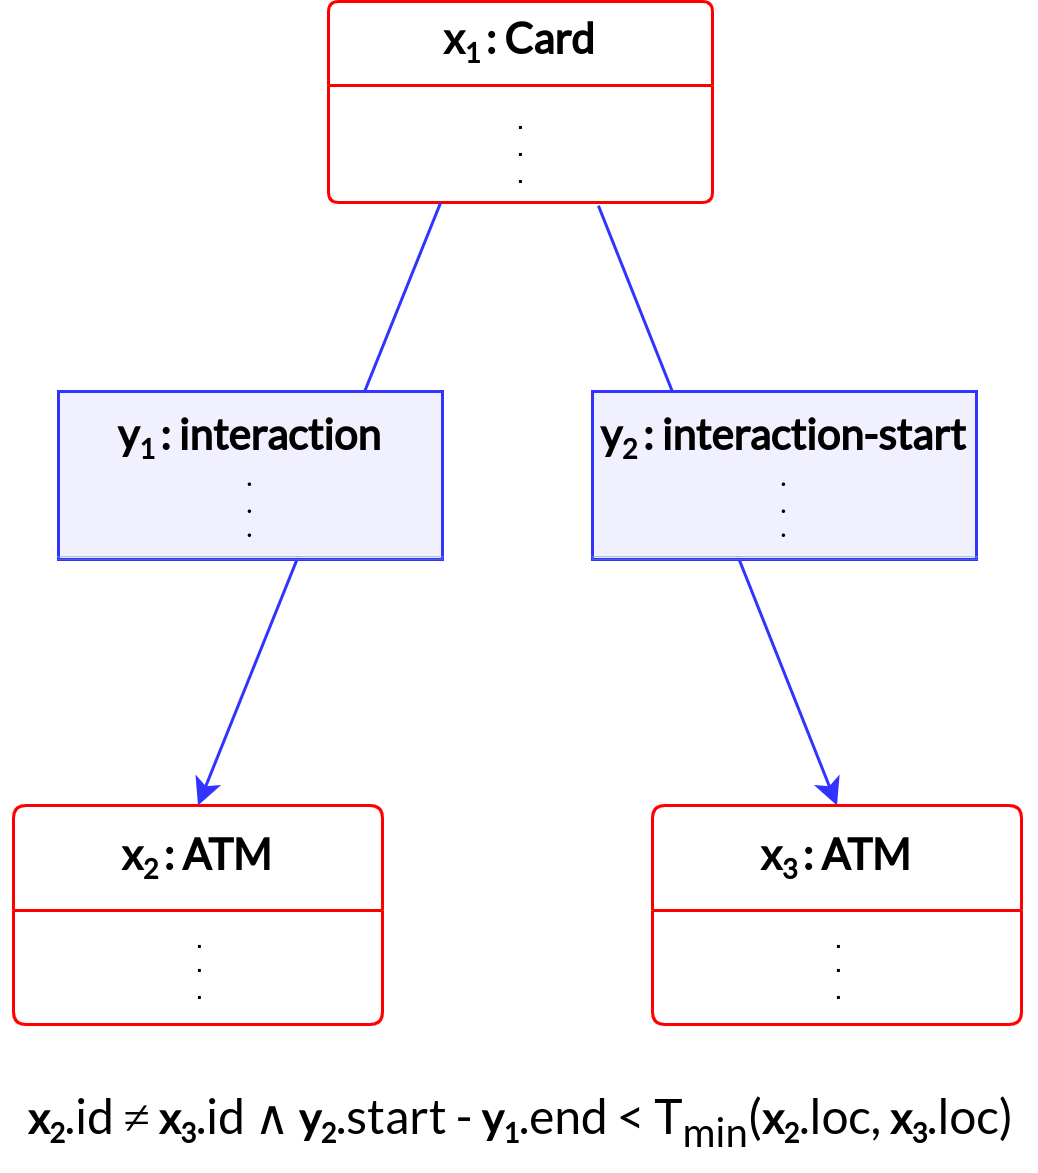
\includegraphics[scale=0.45]{images/2-QueryModel/graphPattern-1.png}
            \caption*{Card cloning}
        \end{figure}
      \end{column}
      \hfill
      % segunda columna
      \begin{column}{0.7\textwidth}   
        \vspace{1.5em}
        \begin{figure}
            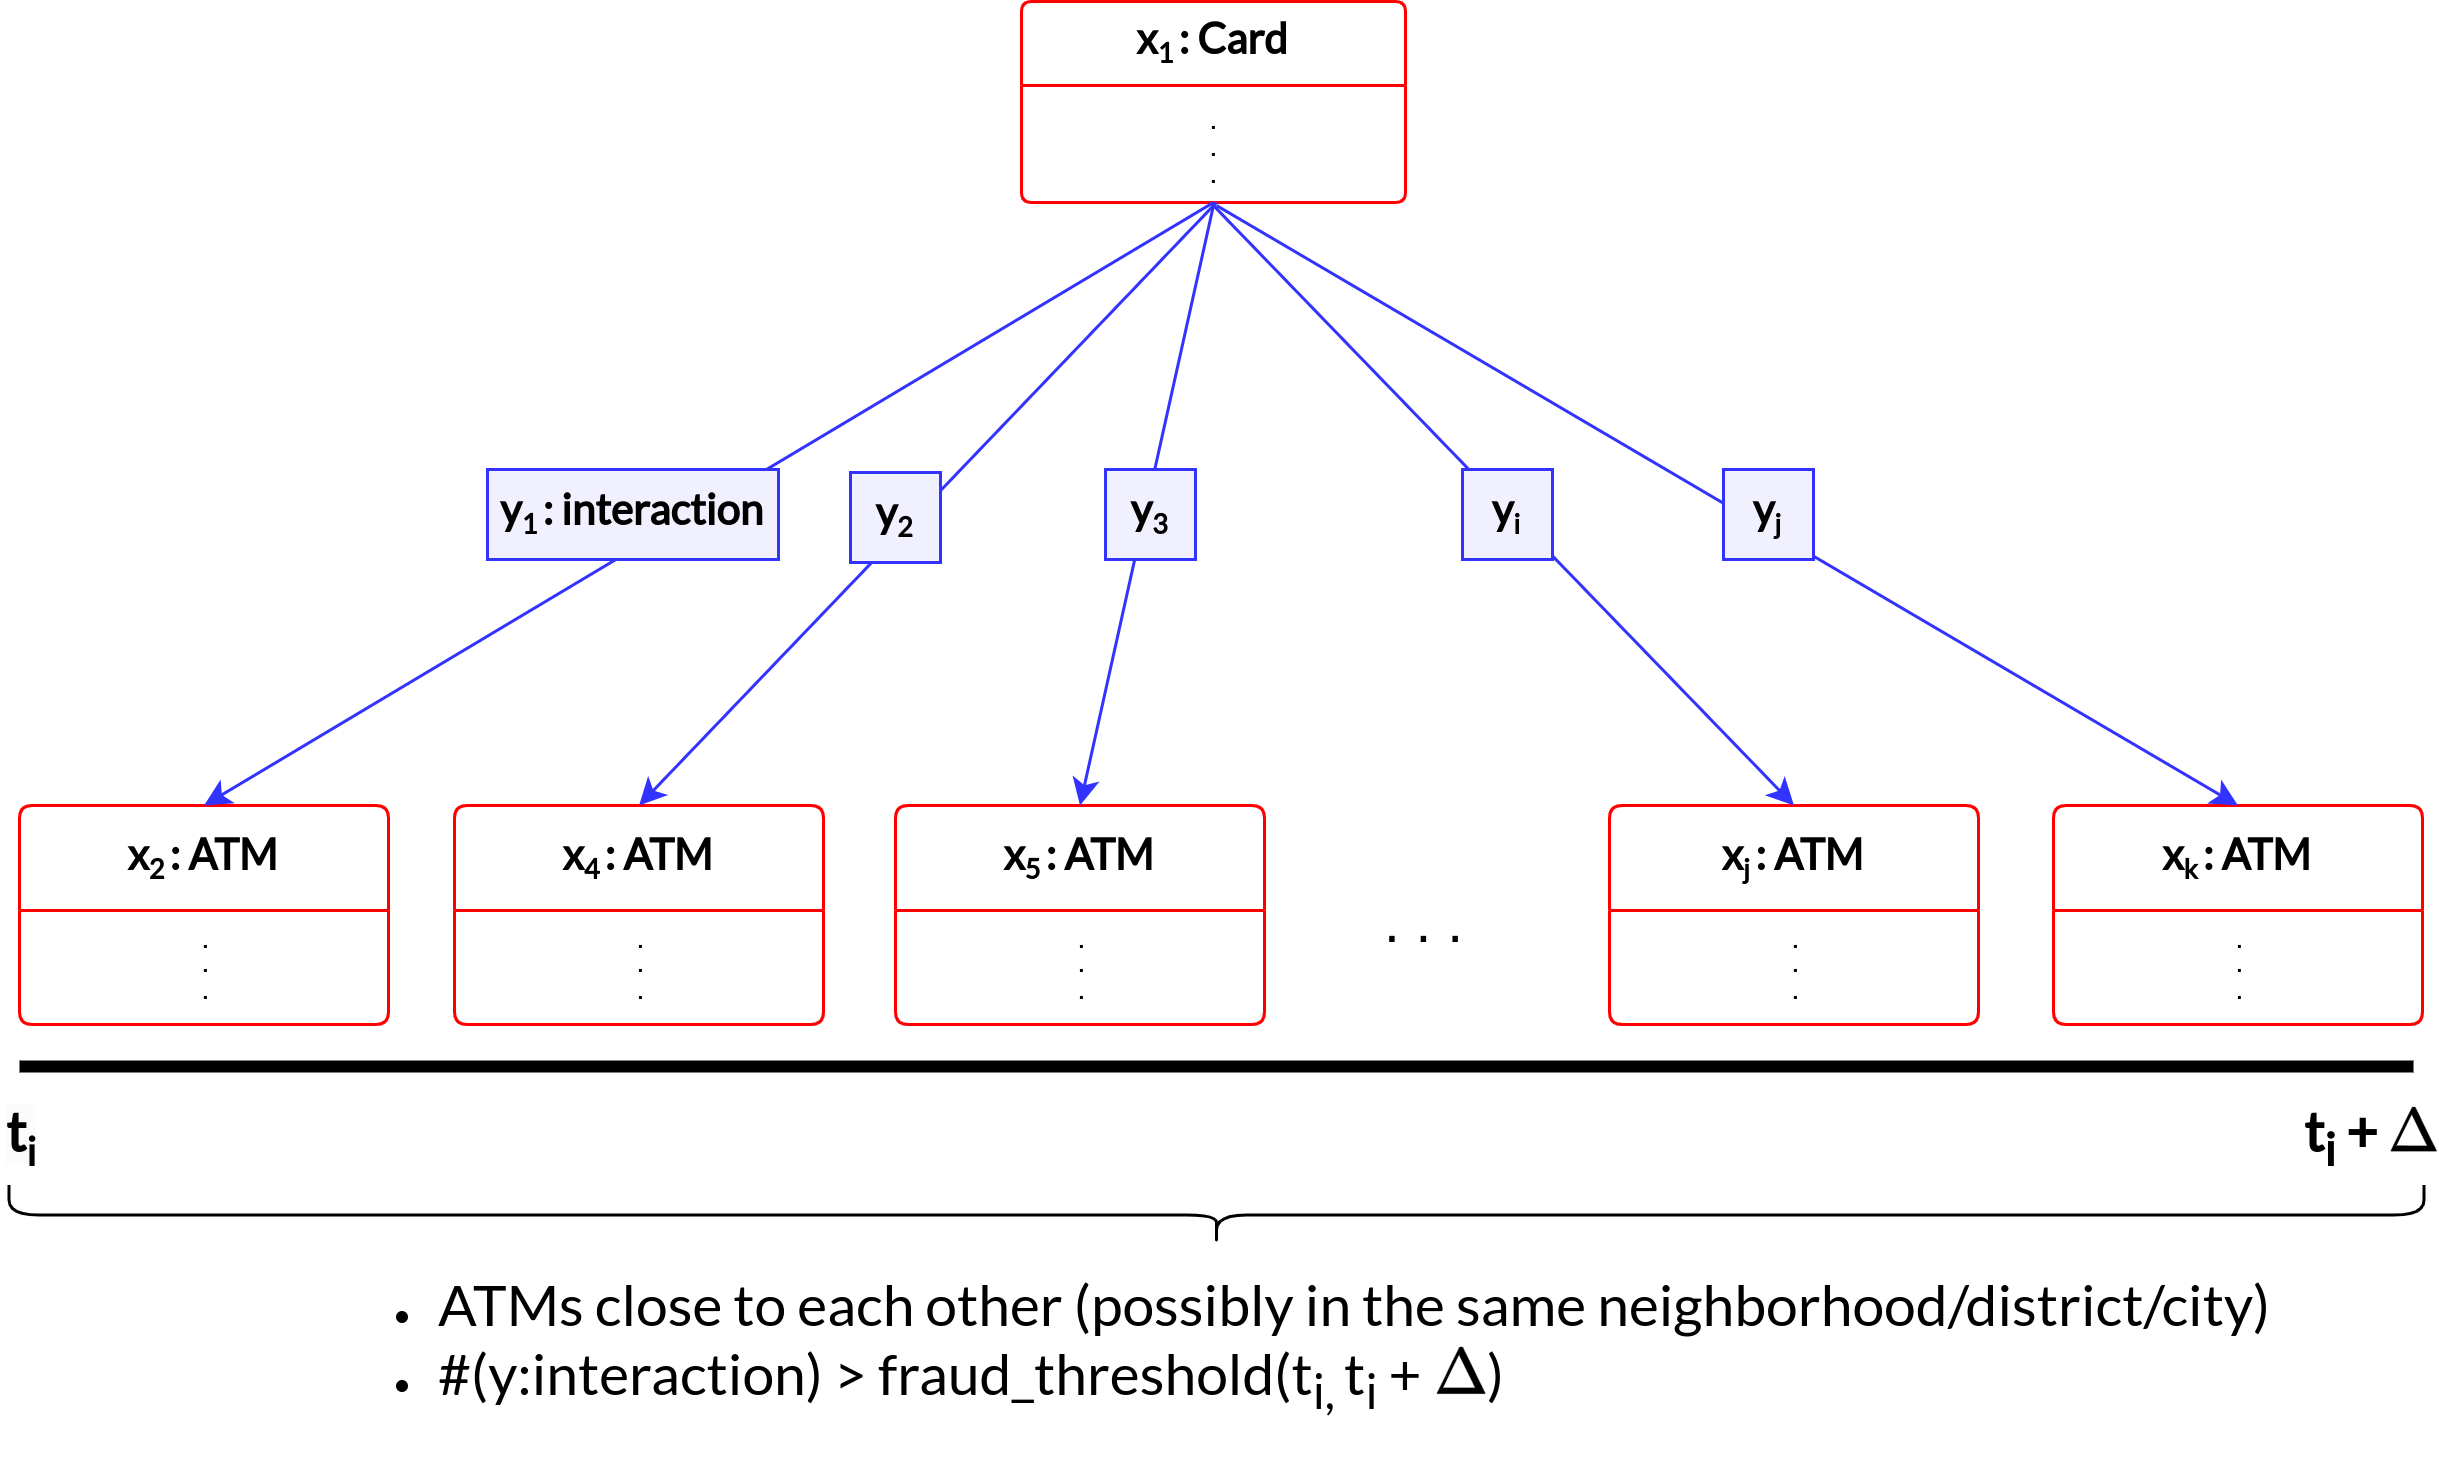
\includegraphics[scale=0.35]{images/2-QueryModel/graphPattern-2.png}
            \caption*{\emph{Lost-and-stolen} card}
        \end{figure}   
      \end{column}
\end{columns}
\end{frame}

\begin{frame}{Proposal: Query Model}
    \begin{itemize}
        \item \textbf{\emph{Continuous query model}}: Fixed queries evaluated over data streams.
        \item Progressive query evaluation process. Based on: \\
        \vspace{0.3em}
        \begin{itemize}
            \item \fbox{Graph pattern matching} in the \textcolor{blue}{volatile subgraph}. \\
            \item[\textcolor{black}{\ding{59}}\hspace*{-6em}] 
            \item \fbox{Satisfiability of constraints} over the properties: possibly querying the \textcolor{blue}{stable graph database} (\textit{retrieve some additional info}).
        \end{itemize}
    \end{itemize}
    \hspace*{1cm}
    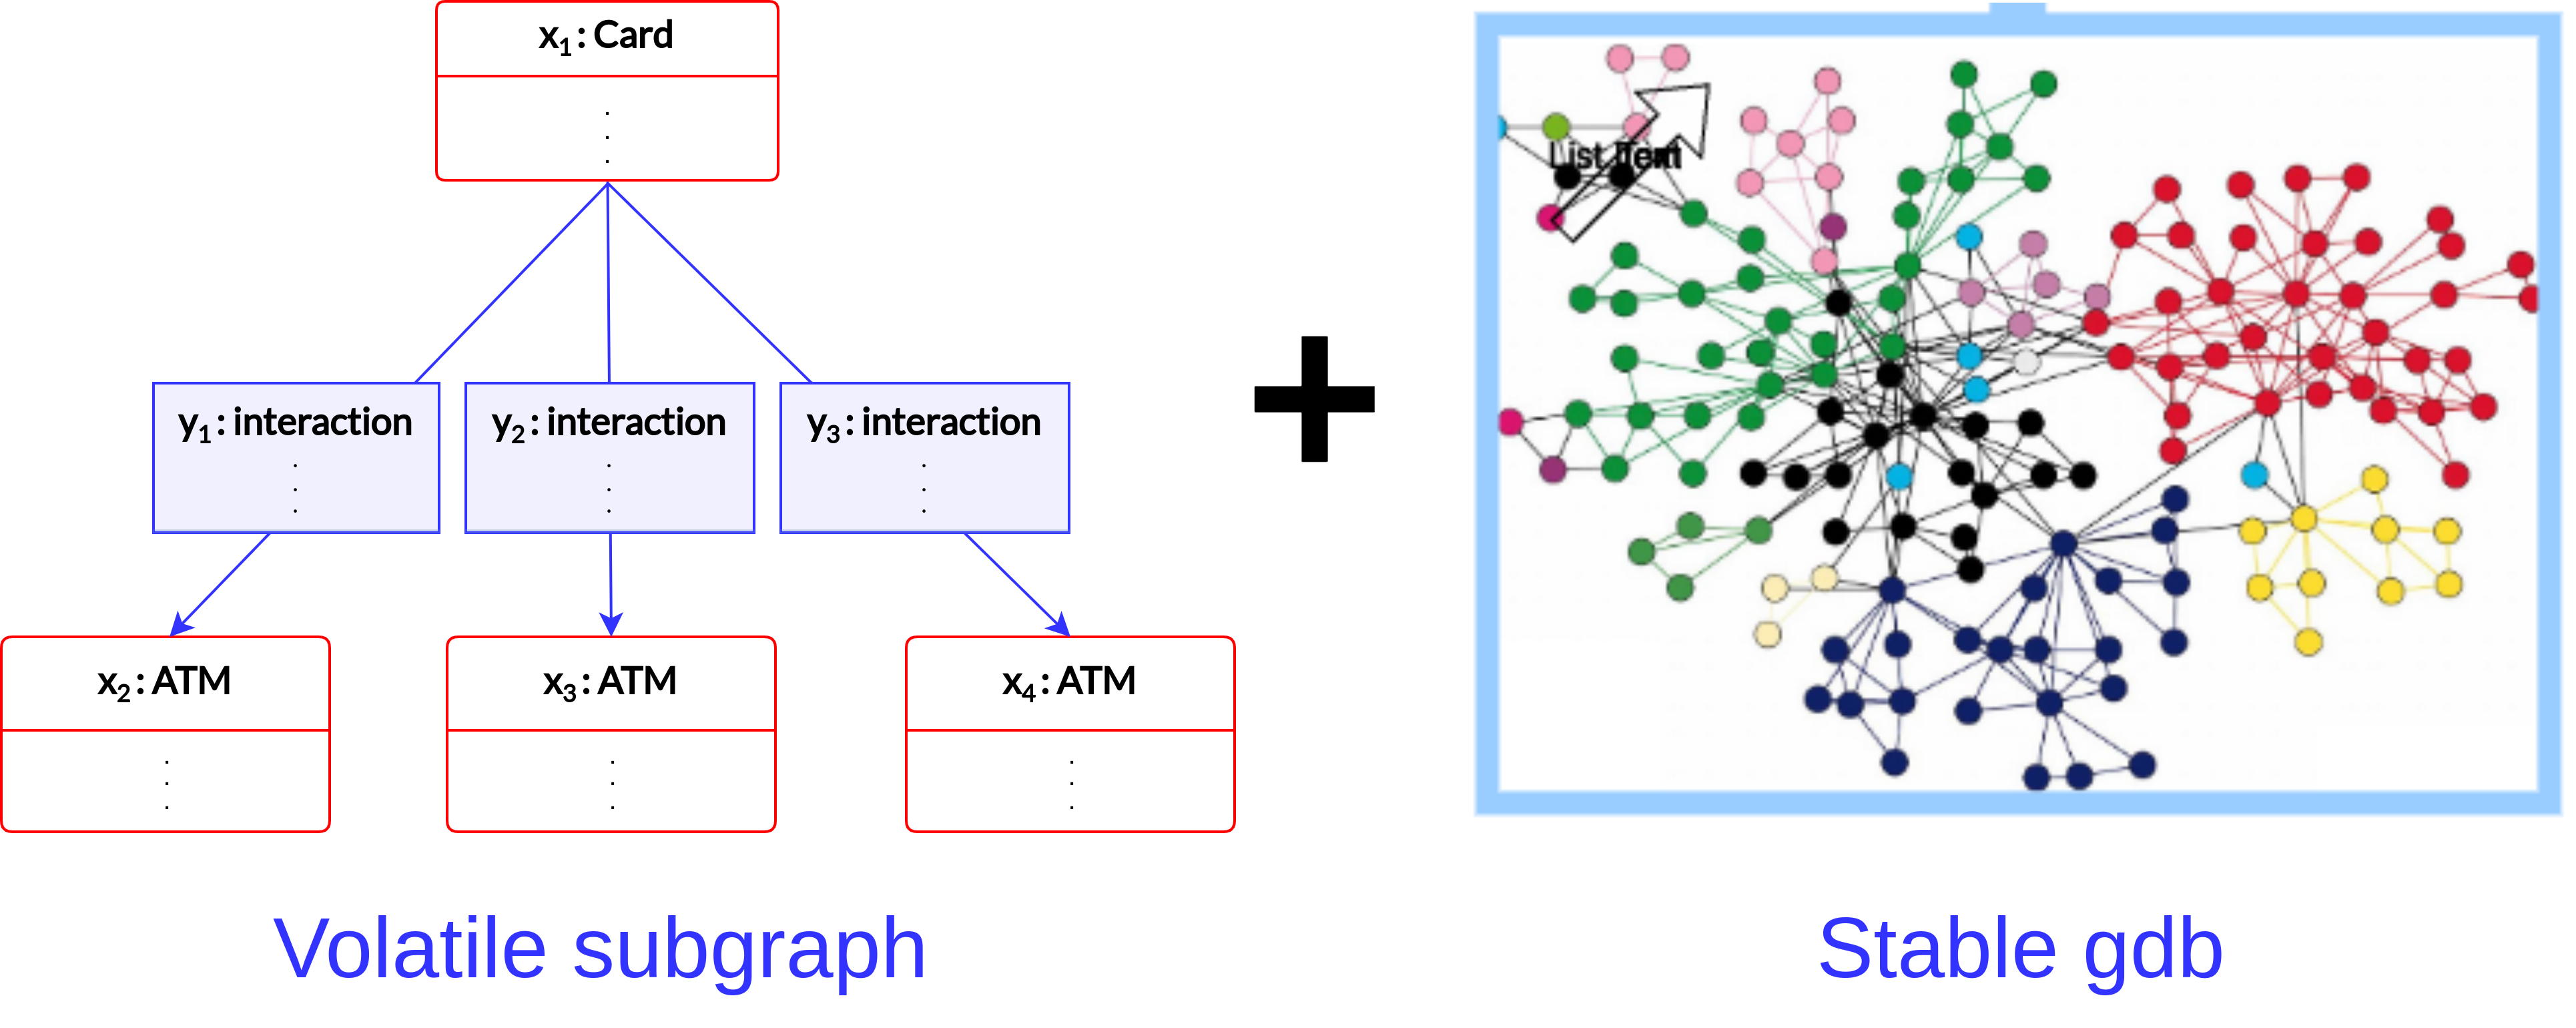
\includegraphics[scale=0.35]{figures/querymodel.png}
\end{frame}

\begin{frame}{Proposal: Query Model}
    \begin{itemize}
        \item Continuous Query Evaluation Engine based on the \textbf{Dynamic Computational Approach} - \cite{Pasarella2024}. 
        \begin{itemize}
            \item Stream processing computational model.
            \item Execution of tasks (query evaluations) concurrently/in-parallel.
        \end{itemize}
    \end{itemize}
\begin{figure}
    \centering
    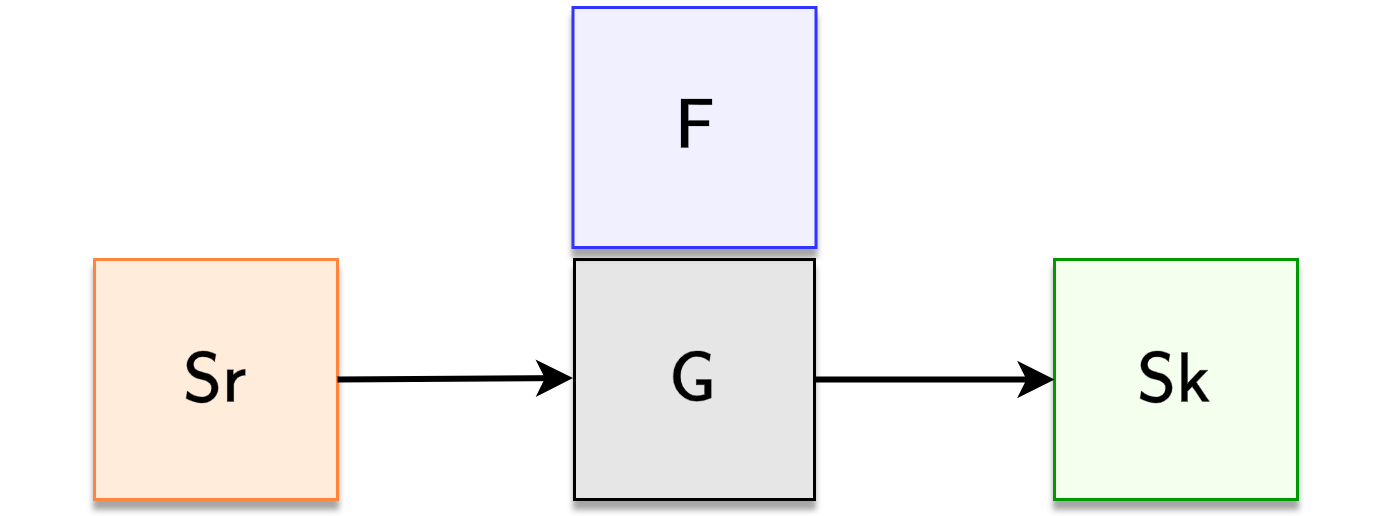
\includegraphics[width=0.55\linewidth]{images/3-Engine/DP-Stages-1.png}
\end{figure}
\vspace{0.2em}
\begin{figure}
    \centering
    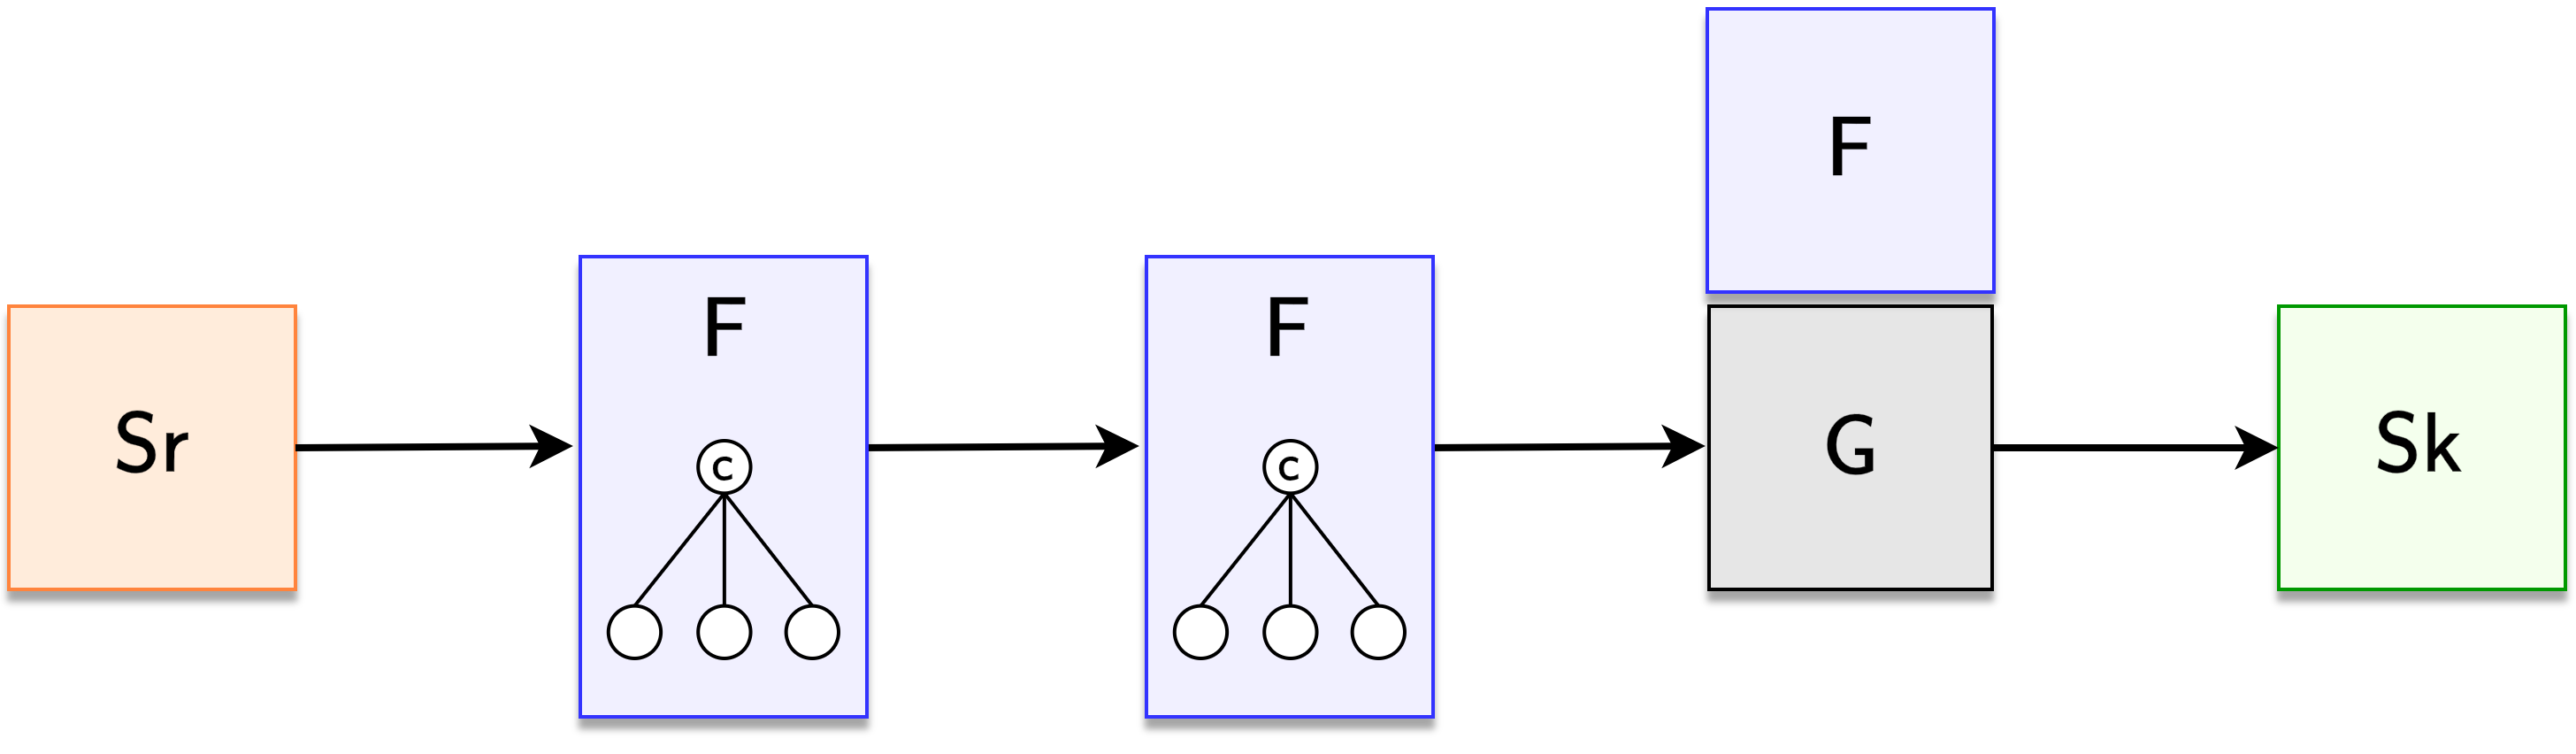
\includegraphics[width=1.0\linewidth]{figures/DP-FilterDetail.png}
\end{figure}
\end{frame}

\begin{comment}
 Royo-Sales \cite{DP-bitriangles2021}
%The problem of progressively identifying and enumerating bitriangles (i.e. a specific graph pattern) in bipartite evolving graphs using the DPA have been successfully solved by Royo-Sales \cite{DP-bitriangles2021}.
%\item Useful to address the problem of evaluating continuous queries over \emph{continuously evolving PGs} (Royo-Sales \cite{DP-bitriangles2021}).
\end{comment}



\newpage

\subsection{Continuous Query Engine - $\mathsf{DP_{ATM}}$}\label{ContinuousQueryEngine}

\textcolor{gray}{To explain:
\begin{itemize}
    \item Encaje/Uso del DP para nuestro engine. Stages, qué hace cada stage (pseudocodigo/algoritmo de cada stage). Canales.
    \item Establecer algoritmos para identificar los patrones asociados a la busqueda de anomalias.
    \item Explicar la idea de que se define como para poder evaluar muchas continuous queries de forma simulatánea (pero que de momento sólo evaluamos una, para nuestro proof of concept)
    \item Detalles más técnicos - Implementación
    \begin{itemize}
        \item Descripción y evaluación del lenguage usado (golang)
        \item Graph-based query language
        \item Tools \& proper system configuration (distintas configuraciones en base al número máximo de tarjetas que contiene cada filtro...)
    \end{itemize}
    \item Windowing?
\end{itemize}
}
\ad{El windowing no lo menciones hasta las conclusiones.}

In this section we define a proper architecture of a continuous query engine for detecting anomalous ATM transactions on a continuous, unbounded, input stream of card-ATM transactions/interactions. We propose an engine that is modeled following the Dynamic Pipeline Paradigm $\mathsf{DPP}$ (see \ref{DPP}), the $\mathsf{DP_{ATM}}$, where, by definition, its architectural framework gets defined as a \DP.\\ 

\fmc{Encaje/Uso del DP para nuestro engine. Volatile subgraphs, cards, filters... Explicar la idea de que se define como para poder evaluar muchas continuous queries de forma simulatánea (pero que de momento sólo evaluamos una, para nuestro proof of concept)}

\fmc{Subgrafos}
The core idea of the \DPATM is to save and construct \emph{volatile} subgraphs of interactions for each of the cards, with the objective to keep track of the ATM transaction/interaction activity of each of the cards of the bank system. The card subgraphs are constructed with the interactions belonging to a certain card. They are defined as \emph{volatile} in the sense that the interactions that compose them are not intended to remain infinitely in the card subgraph, but only for a decided window of time. 
\fmc{Evaluación de muchos tipos de queries de forma simultanea. Un subgrafo por cada tipo de query}
These card subgraphs are the core object on which the detection queries of anomalous PG graph patterns takes place. For each card and for each continuous query pattern, a card subgraph is maintained, allowing the evaluation of many continuous different queries simultaneously. Note that, for each card, a different subgraph for each kind of continuous query is defined due to the possible many distinct time window policies for each particular kind of query.

\fmc{TODO: Poner un dibujo de un subgrafo volátil}

% Descripción general uso DP
To properly characterize the \DP architecture we need to define the configuration and behavior of each of the stages as well as the channels connecting them. The different stages are connected by two communication channels: the \eventch channel carries the interactions of the input data stream and the \alertch channel, which is a direct channel that connects each \emph{Filter} stage with the \sink stage, carries the alerts corresponding to the different possible anomalous transaction patterns detected in a \filter.

\fmc{Duda channels: sólo el de alerts o el de checks. Ahora en la impl tengo checks (incluidos los alerts). Se hizo con la idea de sacar todos los resultados de los checks para ver el continuous delivery of results en los experimentos. Ahora bien, en la impl. final yo diria que solo sacaría las alerts, para tener menos overhead y que el aviso de fraude pudiera llegar antes.}

\ad{Para explicar puedes poner el de checks y que se vea que se van haciendo muchos checks y sólo algunos provocan alerts. Luego puedes explicar que en una "working" version no se pondrías los checks para ser más eficientes y tardar menos en dar los alerts como bien dices.}

Regarding the stages, the \emph{Filter} stage is defined to be the \textit{continuous query evaluator} for a certain subset of bank cards, maintaining the subgraphs for the cards subset that are induced by the interaction edges.

% IDEA GENERAL DP-ATM flow
With this, the \DPATM algorithm overview is as follows: when an interaction $\mathsf{e}$ (with its properties' values) arrives to the \DPATM, the \source stage \Sr registers it into a standard transactional log file. Then, \Sr passes $\mathsf{e}$ to the next stage. If there exists a \filter parameterized with the value of the property \emph{number\_id} of the Card vertex $\mathsf{c}$ that is incident to $\mathsf{e}$, this \filter keeps $\mathsf{e}$ in its state, in particular adding $\mathsf{e}$ to the corresponding card subgraphs. Otherwise, the \filter passes $\mathsf{e}$ to the next stage. In the case of  $\mathsf{e}$ belonging to the \filter, this stage, as the \textit{continuous query evaluator} of the Card $\mathsf{c}$, decides if there is a match with (some of) the continuous query pattern(s) evaluated and emits an alert to the \sink \Sk reporting the finding. Hence, answers are the detected anomalies and they are emitted as they are obtained in filters. When answers/alerts arrive to \Sk, this stage post-processes and output them. In addition, \Sk maintains an answer log file. The fact that an interaction arrives to \G means that there were not previous interactions having the same value of Card property \emph{number\_id} and thus, a new filter parameterized with this new value is spawned. 

\fmc{TODO: Poner imagen de DP con filtros y cada filtro con los subgrafos}

% Descripción más concreta DP...

More detail regarding each of the stages behavior is provided next. An example of the pipeline schema of a \DPATM instance is shown in Figure \ref{img:pipeline-schema}.

\begin{itemize}
    \item \source \Sr: Receives the stream of the card-ATM interactions of the bank. Each interaction $\mathsf{e}$ is represented as an \emph{interaction} relation/edge of the volatile property graph model matching a Card and an ATM \ref{section:volatile-pg}. \Sr registers incoming interaction $\mathsf{e}$ on a transactional log file and passes $\mathsf{e}$ through the \eventch channel to the pipeline.
    \item \filter \F: \emph{Filters} are defined to be the \textit{continuous query evaluators} for a certain subset of the bank system cards. In particular each \F is defined by a subset of root parameters $V_{\mathsf{F}} = \{v_1,\ldots,v_k\}$, representing the Cards being tracked by \F. Therefore, each root represents a Card $\mathsf{c}$ where $v_i$ is the Card property \emph{number\_id} value: $v_i = \mathsf{c}$.\emph{number\_id}. Each \filter is defined to have a maximum capacity in terms of cards being tracked. This maximum capacity is defined by the parameter \emph{maxFilterSize}. This limits the maximum size of the subset $V_{\mathsf{F}}$, so that $|V_{\mathsf{F}}| \leq $ \emph{maxFilterSize}.

    With this, whenever an interaction $\mathsf{e}$ coming from the pipeline reaches \filter \F, it firsts checks whether $\mathsf{e}$ belongs to \filter \F. This is the case when $\mathsf{e}$ is incident to one of the roots of $V_{\mathsf{F}}$, $v_i$, which has the same \emph{number\_id} property value as the Card $\mathsf{c}$ of the interaction $\mathsf{e}$ ($\mathsf{e}$.\emph{number\_id}), that is when $v_i =\mathsf{e}$.\emph{number\_id}. This means that \F is currently tracking the activity of the Card $\mathsf{c}$ to which the interaction $\mathsf{e}$ belongs. 

    \fmc{Se explica cómo se tiene hasta ahora. Pero se debería de explicar una propuesta para el caso en el que se dejara de trackear la actividad de una tarjeta / cómo sería el proceso para poder destruir un filtro/reducir el pipeline.\\
    \textbf{Hasta ahora}: If the filter is not full then we add the not belonging cards to it, until it is full. This is what is done so far, since we are not considering the case to shrink the pipeline. On which some cards activity will be stopped to being tracked. \\
    TODO: Definir una posible propuesta para esto en el caso de que se hiciera... relacionado con lo de la ventana...\\
    - Spawning case is well defined.\\
    - Shrinking case idea: all the cards of the filter have to be "outdated" so that the filter can be eliminated... (not done for the moment, infinite window considered)
    }
    Another possible case on which $\mathsf{e}$ is decided to belong to \filter \F, is when, although the Card $\mathsf{c}$ of $\mathsf{e}$ is not currently being tracked by \F, it is decided to start doing it since \F still has the capacity to track more cards: $|V_{\mathsf{F}}| < $ \emph{maxFilterSize}. Therefore, card $\mathsf{c}$ is introduced as a new root parameter $v_{k+1} = \mathsf{e}$.\emph{number\_id} to $V_{\mathsf{F}}$: $V_{\mathsf{F}} = V_{\mathsf{F}} \cup v_{k+1}$. These two belonging conditions are summarized as:
    
    $$
    \mathsf{e} \in \mathsf{F} \iff 
    \left(\exists v_i \in V_{\mathsf{F}} \text{ such that } v_i = \mathsf{e}.\emph{number\_id} \right) 
    \lor \left(|V_{\mathsf{F}}| < \emph{maxFilterSize}\right).
    $$

    Otherwise ($\nexists v_i \in V_{\mathsf{F}} \text{ such that } v_i = \mathsf{e}.\emph{number\_id} \land |V_{\mathsf{F}}| = $ \emph{maxFilterSize}), \F passes $\mathsf{e}$ to the next stage.

    In the case of $\mathsf{e}$ belonging to \F, \F checks if there is a match with (some of) the continuous query pattern(s) evaluated and emits an alert(s) to the \sink \Sk. For this, $\mathsf{e}$ will be added to the corresponding card $\mathsf{c}$ subgraph(s) with root $v_i =\mathsf{e}$.\emph{number\_id}, and then perform the algorithm to test (each of) the continuous query pattern(s) with their associated card $\mathsf{c}$ subgraph(s). 

    \fmc{Esto justificarlo así?}
    For a card $\mathsf{c}$, we will store one different subgraph for each of the continuous query patterns evaluated. A different subgraph for each of the continuous query patterns is needed since the evaluation politics of each of the patterns may be different. For instance, for a specific pattern we may need to store a full list of interaction edges with some specific properties, whereas for others only the last interaction edge. Or even just some specific properties and not a subgraph of interactions. This will depend on the definition on each of the specific continuous query patterns considered.

    The test of a continuous query pattern is done by means of its associated card \emph{continuous query pattern subgraph} stored by \F and the information retrieved from the stable PG to identify patterns and solve constraints. This is, indeed, the way to evaluate continuous queries.
    
    \item \generator \G: Is the stage in charge of stretching the pipeline by spawning new \filter \F stages when needed. In particular this is the case whenever an interaction $\mathsf{e}$ arrives to \G. At this point this means that there was no \F in the pipeline to which this interaction belonged. That is, whenever no \F was tracking the activity of the Card $\mathsf{c}$ with property value \emph{number\_id} to which this interaction corresponds and all the running \F were full of capacity in terms of the number of maximum cards \emph{maxFilterSize} that they can track. In this case a new \F is spawned, initially tracking the activity of this Card $\mathsf{c}$ with property value \emph{number\_id} and creating new card subgraphs with the interaction $\mathsf{e}$. 
    \item \sink \Sk: It is in charge of receiving all the alerts coming from the \filter stages and to correspondingly act on them as the bank requires. This could be done in terms of communicating the alert to the corresponding cardholders, emitting a message for validating that the operation was done by the owner, freezing the corresponding cards, and so on. This will have to be defined by the corresponding bank as desired. In any case, \Sk maintains an answer log file where all the emitted alerts are registered. Additionally, an event log file is maintained, to register other internal system events.
\end{itemize}


\begin{figure}[H]
    \centering
    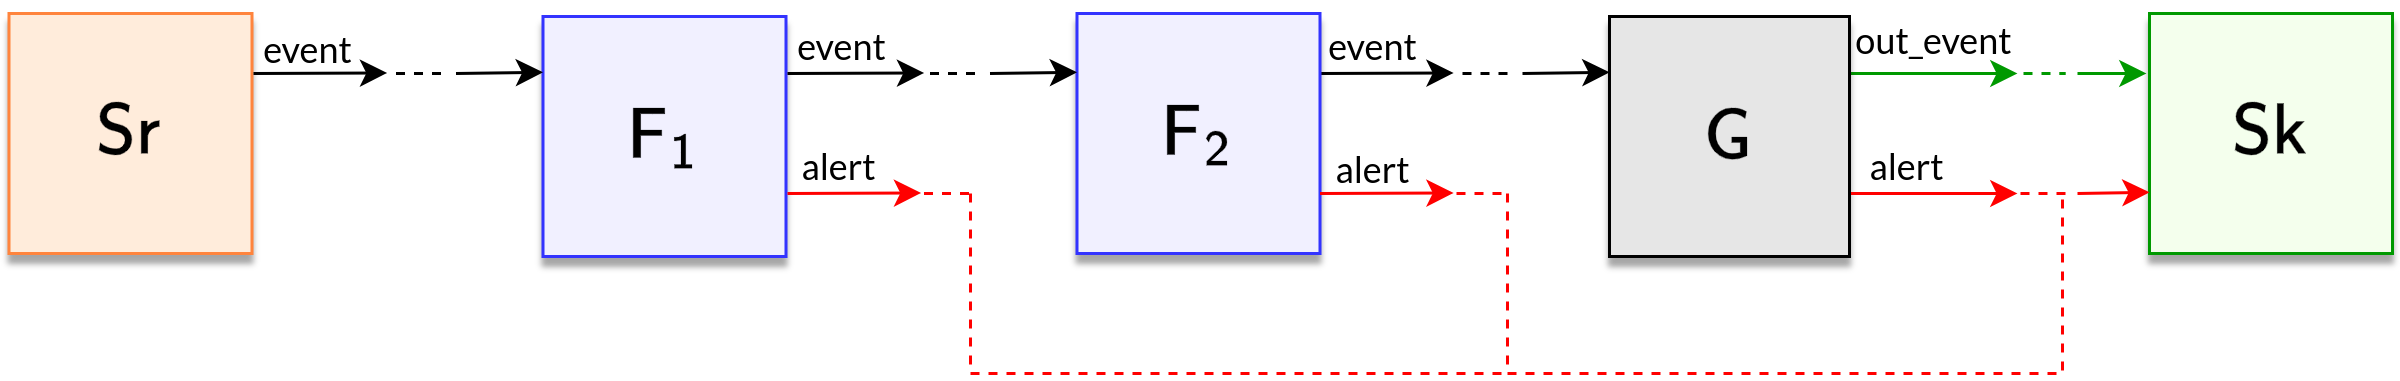
\includegraphics[scale = 0.8]{images/3-Engine/DP-2f.png}
    \caption{Example of the Pipeline Schema of a \DPATM Instance}
    \label{img:pipeline-schema}
\end{figure}


\fmc{Windowing?}
When the time interval window is over, the $\mathsf{DP_{ATM}}$ is, in some sense, reset according to the given window policy. Note that the window policy must take into account stored data that might be valid in between two windows and handle the transition properly.

\fmc{Detalles técnicos - Implementación}
\subsection*{$\mathsf{DP_{ATM}}$ - Implementation}\label{ContinuousQueryEngine-Implementation}

% Lenguaje de programación. Base de datos. Conexión a base de datos.
% - Go: Detalles versión. Por qué lo usamos
% - Neo4j: Detalles versión. Por qué lo usamos
The implementation of the proof of concept can be found in Github\footnote{\url{https://github.com/FCanfran/ATM-DP}}. It was developed using the version \texttt{1.20} of the \texttt{Golang} language. 
% Ventajas: hilos verdes - concurrencia, comunicación entre stages con canales de fácil manejo, fácil conexión con Neo4j mediante el driver
One of the main reasons why we decided to use this language is its inherent capacity to support concurrent programming \cite{Go-cbtnuggets_concurrency, Go-medium_concurrency, Go-reliasoftware_concurrency}, which is the computing technique that we need to implement the \DP schema for our \DPATM engine. In \texttt{Go}, concurrency is achieved primarly through \texttt{goroutines} and \texttt{channels}. \texttt{Goroutines} are lightweight, independent concurrent green threads, which are managed by the \texttt{Go} runtime scheduler, and enable concurrent execution of functions, in our case stages. The communication between \texttt{goroutines} is accomplished via different channels. This provides a safe and efficient method to pass complex data between the different \texttt{goroutines}. 
Unlike traditional threads, \texttt{goroutines} have a small memory footprint and can be created in large numbers with minimal overhead. The \texttt{Go} runtime includes an efficient scheduler that multiplexes \texttt{goroutines} onto CPU cores, reducing context switching overhead and optimizing resource use. However note that, \texttt{goroutines} are not inherently parallel. By default, \texttt{Go} uses only one operating system thread, regardless of the number of \texttt{goroutines}. We need to set up the \texttt{GOMAXPROCS} \footnote{\url{https://pkg.go.dev/runtime\#GOMAXPROCS}} environment variable to the number of logical processors, to achieve that the \texttt{Go} runtime scheduler multiplexes the \texttt{goroutines} onto all the possible logical processors specified.\\

Another advantage that made the election of \texttt{Go} quite suitable was its easy form to interact with \texttt{Neo4j}. \texttt{Go} provides the \texttt{Neo4j Go driver}\footnote{\url{https://neo4j.com/docs/go-manual/current/}} to easily interact with a Neo4j instance through a \texttt{Go} application. More details regarding the connection are later explained. 

\subsubsection*{Neo4j Connection}\label{Neo4j-connection}
% Detalle de la conexión con Neo4j
Our \DPATM system needs a way to interact with the stable bank database PG instance in order to retrieve additional information related with the cardholders or ATMs for the evaluation of the continuous queries. The connection to the Neo4j graph database instance that represents the stable bank PG database is implemented using the version \texttt{v5.24.0} of the \texttt{Neo4j Go driver}\footnote{\url{https://pkg.go.dev/github.com/neo4j/neo4j-go-driver/v5@v5.24.0/neo4j}}. Next we give an overview of some important details on the usage of this driver in order to connect and query the Neo4j instance. More detail on the methods we used can be found in the official driver module websites \cite{neo4j-go-neo4j_go_driver, neo4j-go-neo4j_go_manual}.\\


In our implementation of the \DPATM system in \texttt{Go} we developed the \texttt{Go} module \texttt{internal/connection} to deal with the connection management with the Neo4j stable bank graph database instance.
On it we provide all the needed functions to connect to the database, create connection sessions, and to query it. 

% Initial connection method - .env... driverwithcontext
% Sessions for each of the filters
% Query method to run cypher queries...

\begin{itemize}
    \item \textbf{Initial connection setup}: The \DPATM system initially sets up the connection through the creation of a \texttt{DriverWithContext} object.\\
    In the \texttt{internal/connection} module \texttt{SafeConnect()} is the function that we implement to construct the \texttt{DriverWithContext} object and verifies that a working connection can be established through the \texttt{.VerifyConnectivity()} method.
    The \texttt{DriverWithContext} object holds the details required to establish connections with a Neo4j database, allowing connections and creation of sessions. It is a sharable object among threads. To provide the required details we used the module package \texttt{godotenv}\footnote{\url{https://pkg.go.dev/github.com/joho/godotenv}} to obtain the \textit{URI} and the credentials from a \texttt{.env} file, where the related environment variables are specified. For the connection with our Neo4j instance we use the \texttt{Bolt}\footnote{\url{https://neo4j.com/docs/bolt/current/bolt/}} application protocol, which is the protocol used for interaction between Neo4j instances and drivers. It listens on port 7687 by default. 
    To illustrate, we show an example of a \texttt{.env} file, from which the connection credentials will be gathered by our application. On it the connection details of a toy local Neo4j instance are shared:

    \begin{center}
    \lstset{style=cypherStyle}
    \begin{lstlisting}[caption={Example of a \texttt{.env} file, from which from which the connection credentials will be gathered by our \DPATM application.}]
        NEO4J_URI="bolt://localhost:7687"
        NEO4J_USERNAME="neo4j"
        NEO4J_PASSWORD="xxxxx"
    \end{lstlisting}
    \end{center}

    \item \textbf{Connection sessions}: \texttt{Sessions} act as concrete query channels between the driver(\texttt{DriverWithContext} object) and the server. We need them in order to be able to run \texttt{Cypher} queries from each of the working \filter stages. Each \filter stage creates a different \texttt{session} to interact with the Neo4j database.
    
    In the \texttt{internal/connection} module, the functions \texttt{CreateSession(...)} and \texttt{CloseSession(...)} are the functions for the creation and closing of a \texttt{session}.
    They are created from the \texttt{DriverWithContext} object. 

    \item \textbf{Running queries}: We provide the methods \texttt{ReadQuery(...)} and \texttt{WriteQuery(...)}, which create a \textit{managed transaction} to retrieve data from the database or alter it, respectively, through a \texttt{Cypher} statement. 
    Internally they call the \texttt{ExecuteRead(...)} and the \texttt{ExecuteWrite(...)} functions of the \texttt{Neo4j Go Driver}, which execute the given unit of work in a read/write transaction, via the provided session.

    In the \DPATM we make use of the \texttt{ReadQuery(...)} function from each of the \filter stages, using its own \texttt{session}, to query the database using \texttt{Cypher} statements.
\end{itemize}

\fmc{DUDA: Pongo una referencia a esto?}
\textcolor{gray}{Neo4j limits the number of parallel transactions to 1000 by default. However, so far no reference regarding the limit on the number of parallel sessions has been found. In any case, it is important to remark that many multiple parallel sessions may cause overhead to the database. This can be the case for the architectural design we are proposing, where we have a session per each \filter stage.}

% Comunicación. Canales, tipos más concretos. Eventos, tipos de eventos concretos. Start and End Edges.
\subsubsection*{Communication}

The communication of the different stages is carried via different \texttt{Go} channels. In general, although otherwise specified all the channels that we use are buffered channels of size 5000. All the channels are described next:

\begin{itemize}
    \item \eventch: \texttt{event} channel. Its main purpose is to carry the interaction edges across the \DP stages, from \Sr to \G, passing by all the \F's. The \texttt{event} data type consists on a \texttt{EventType} label and in a \texttt{Edge} object. The \texttt{EventType} label indicates the type of event that can be either: \texttt{EdgeStart} representing an opening of an interaction, \texttt{EdgeEnd} representing an interaction closing, \texttt{EOF}, representing the \textit{End Of File} event so that the \DP can become to an end, finalizing all the stages, and the \texttt{LOG} event for internal log messages of the system.
    \begin{center}
    \lstset{style=golangStyle}
    \begin{lstlisting}[caption={\texttt{Event} Data Type}]
                type Event struct {
            	   Type      EventType
            	   E         Edge
                }
    \end{lstlisting}
    \end{center}

    \texttt{Edge} is the data type that we defined for the interaction edges. This object will be relevant in the case of the \texttt{EdgeStart} and \texttt{EdgeEnd} events, since in this case the \texttt{Edge} object will be containing the information of the opening and closing interaction, respectively, as defined in the volatile property graph data model definition (see \ref{section:volatile-pg}).
    
    % Tipo de dato interaction edge Edge
    \begin{center}
    \lstset{style=golangStyle}
    \begin{lstlisting}[caption={Data Type for the interaction edges in Go}]
    type Edge struct {
    Number_id string   // Card id
    ATM_id   string    // ATM id
    Tx_id    int32     // id
    Tx_type  TxType    // type (withdrawal/deposit/inquiry/transfer)
    Tx_start time.Time // start datetime(DD/MM/YYYY HH:MM:SS)
    Tx_end   time.Time // end datetime(DD/MM/YYYY HH:MM:SS)
    Tx_amount float32  // amount
    }
    \end{lstlisting}
    \end{center}

    where \texttt{TxType} is a custom type made for the different interaction types: 
    \texttt{withdrawal}, \texttt{withdrawal}, \texttt{withdrawal} and  \texttt{withdrawal}. 

    \begin{center}
    \lstset{style=golangStyle}
    \begin{lstlisting}[caption={\texttt{TxType} Data Type, for the different interaction types}]
            type TxType uint8
            const (
            	Withdrawal TxType = 0
            	Deposit           = 1
            	Inquiry           = 2
            	Transfer          = 3
            	Other             = 4
            )
    \end{lstlisting}
    \end{center}
    
    \item \alertch: \texttt{alert} channel. It carries the alerts corresponding to the different possible anomalous transaction patterns detected in a \filter. It is a channel directly connecting each of the \emph{Filters} with the Sink stage. This means that when an alert is emitted it does not have to travel through all the remaining \F stages of the \DP nor the \G stage, allowing a faster communication of the alert to the \Sk stage, in charge of processing the alerts. The \texttt{alert} data type consists on a \texttt{Label} to indicate the type of fraud pattern to which it corresponds, an \texttt{Info} string to indicate additional information related with the alert, and finally \texttt{Subgraph}, the subgraph data structure that triggered the alert. Note that this subgraph does not need to be the full subgraph of the card that triggered the alert, it can be just the part of it involved in the alert. For instance, in the case of the fraud pattern I, these subgraph is composed of the two interaction edges that caused the trigger of this kind of fraud pattern alert.
    \begin{center}
    \lstset{style=golangStyle}
    \begin{lstlisting}[caption={\texttt{Alert} Data Type}]
    type Alert struct {
    	Label    string        
    	Info     string        
    	Subgraph Graph         
    }
    \end{lstlisting}
    \end{center}
    \item $\mathsf{out\_event}$: direct dedicated \texttt{event} channel between the \G and \Sk. 
    \item $\mathsf{internal\_edge}$: Internal \texttt{event} channel between a \F stage and its related \FW substage. It only pass interaction \texttt{Edge} events (\texttt{EdgeStart} and \texttt{EdgeEnd}), that have been determined to belong to the \filter, so that the related \FW of \F can do the corresponding processing with it.
  \end{itemize}

% Detalle de las estructuras y los métodos usados en cada una de las stages.
\subsubsection*{Stages}
In what follows we give specific implementation details of each of the stages of the \DP paradigm used for the \DPATM. Each stage takes the form of a \texttt{goroutine} of the \texttt{Go} language.

% - Source: como se hace la lectura. Como se empezó haciendo inicialmente y cómo se decidió hacer finalmente (lectura por chunks) - hacer referencia a apartado de experimentos donde mostrar el experimento hecho para enseñar que era mejor.
\paragraph*{Source\\ }

% Explicar función

\source stage is designed to be the connection point of the \DPATM with the bank ATM network to receive the interactions produced on these ATMs, which compose the input interaction stream.\\

\fmc{DUDA: Aqui esto no se como ponerlo...
- Decir algo de kafka message queue (como en seraph)?
}
% Forma real de cómo sería el source: recibiendo flujo de transacciones en real time
% Cómo lo hacemos nosotros - lectura de fichero - y variantes dependiendo del tipo de experimento que realizamos
In a real-case scenario, these interaction events could be sent by the ATMs of the bank network and be received by a message queue on our \DPATM system. For our proof of concept, where we generated our own synthetic stream of transactions in a \texttt{csv} file,
the interactions are read from these files, parsed into \texttt{Edge} data types and provided to the pipeline in different ways depending on the kind of simulation we perform. As it will be shown in the Experiments section, we implemented two different cases of simulations. The real-case scenario and the high loaded test scenario. In the first case, the interactions, although read by a file of artificial simulated interactions, are provided to the pipeline data stream in such a way that they simulate their actual arrival time to the system, with the corresponding time separation between them. In the second case, the interactions are provided just one after the other as fast as possible as they are read.\\

% Cómo se leen, parsing al tipo de dato Edge...
In any case, we want the reading of the input file to be the fastest possible, so to minimize the potential bottleneck derived from the operation of reading a file, we utilized a buffered reader of the \texttt{bufio} package, which reads chunks of data into memory, providing buffered access to the file. This buffered reader was provided to a \texttt{csv} reader of the \texttt{encoding/csv} package to read the buffered stream as \texttt{csv} records.

    \begin{center}
    \lstset{style=golangStyle}
    \begin{lstlisting}[caption={\texttt{csv-bufio} reader}]
        reader := csv.NewReader(bufio.NewReader(file))
    \end{lstlisting}
    \end{center}
    
% Lectura por chunks
% chunk size = 100
% read with the help of a worker to keep reading in the background, to accelerate the reading -> explain the reason of why this
Another optimization that was done in order to be able to minimize this bottleneck on the reading of the interactions from the \texttt{csv} file, was reading by chunks the \texttt{csv} records/rows. In particular, this was done by having a \textit{worker} subprocess, implemented as an anonymous \texttt{goroutine} inside \Sr, whose task was to continuously read records from the file using the \texttt{csv-bufio} reader accumulating them in a chunk of rows that were provided through a channel to \Sr whenever they reached the defined \emph{chunkSize}. These records were read directly as \texttt{string} data types. On its side, whenever \Sr receives a chunk of rows, it takes each of the rows on it, parses it to the \texttt{Edge} data type and sends it through the pipeline to the next stage.\\

The \emph{chunkSize} was selected to be of $10^2$ rows. In \ref{input-reading} we provide an experimental analysis that proves and justifies the benefits of this buffered and chunked file reading. On it the \texttt{encoding/csv} package performance is compared to other variants using the \texttt{apache/arrow} package with different combinations of \emph{chunkSize}. We also analyze the benefits of introducing the \textit{worker} subprocess to perform the chunked reading.

\fmc{Explicar más en detalle como va lo de la lectura por chunks con el worker?}







% - Filter: forma inicial - sin filter worker y 1 card per filter - y mejoras posteriores con filter-worker y varias cards por filtro con un hash map para indexar... Poner esquema/algoritmo final del filtro (con referencia al algoritmo de FP definido en el query model).
\paragraph*{Filter\\}

Regarding the \filter stage, there are four main aspects worthy to describe on its implementation: the card subgraph data structure implementation, the \emph{decoupled event handling} implementation, the \filter multiple cards support and the continuous query evaluation.
\begin{itemize}
    \item \textbf{Card Subgraph Data Structure}\\
    It contains the interaction edges related with the continuous query fraud pattern evaluation of a specific card.
    The card subgraph data structure is selected based on the fraud patterns considered so far. Although for the implementation of the detection of the fraud pattern I (see \ref{section:queryModel}) we only need to store the last/most recent interaction for each card, we propose a \texttt{Go} \texttt{list} of \texttt{Edge} (interaction edges) objects as a more general data structure to store incoming interactions ordered by timestamp. This decision responds to what we see it is a more general data structure ready for its usage when implementing the detection of other kinds of fraud patterns.\\ 

    \begin{center}
    \lstset{style=golangStyle}
    \begin{lstlisting}[caption={Card Subgraph Data Structure in Go}]
    type Graph struct {
    	edges *list.List 
    }
    \end{lstlisting}
    \end{center}

    A card subgraph is constructed based on the belonging interaction edges that arrive in the form of incoming \texttt{EdgeStart} and \texttt{EdgeEnd} events. \texttt{EdgeStart} event  produces the creation of a new \texttt{Edge} on the data structure, whereas a \texttt{EdgeEnd} event completeS the values of the properties of the corresponding \texttt{Edge} on the data structure, that was previously created by the \texttt{EdgeStart} event corresponding to that same ATM-Card interaction.

    \fmc{TODO: Poner dibujito de subgrafos dentro del filtro?}

    \item \textbf{Decoupled Event Handling}\\
    % Filter worker
    We implement a \emph{Decoupled Event Handling}, as in the \DP implemented on \cite{DP-Benedi_Garcia_2024}. As the authors mention in this work, there exists a potential inefficiency in the way that the \filter \F stage is defined to work: if an event belongs to the filter then it does the processing related to it. Until \F does not complete this processing the events that arrive to it are not being able to be handled, even if the event does not belong to \F. We have the same scenario for the \DP of the \DPATM, where the events that can belong to \F are the interaction edge $\mathsf{e}$ events.

    To avoid this bottleneck on the flow of interaction edge $\mathsf{e}$ events, the \filterworker \FW is introduced as a substage of the \filter \F stage. \F and its associated \FW will be running in different \texttt{goroutines}. The idea is that \F acts as a dedicated \textit{mailbox}, reading the events coming from the \texttt{event} channel and \emph{filtering} them, that is, deciding whether an incoming interaction edge $\mathsf{e}$ belongs to \F or not. In the case $\mathsf{e}$ belongs to \F, \F forwards $\mathsf{e}$ to the \FW, otherwise it continues passing $\mathsf{e}$ through the pipeline. \FW is dedicated to do the corresponding processing with the interaction edges belonging to the stage that are forwarded by \F.\\

    This decoupling allows to do the processing of belonging interaction edges while not blocking the pipeline event flow, since at the same time it does the \emph{filtering} of events.\\

    In our \texttt{Go} implementation, we decided to implement \FW as an internal anonymous \texttt{goroutine} of the \F \texttt{goroutine}, instead of an external (named) \texttt{goroutine}. 

    To communicate the interaction edges between \F and \FW we use an internal channel \internaledgech. Another possible option considered was a shared buffer of interaction edges. In this last case a mutex would have been needed, since \F and \FW can possible write and read, respectively, into this buffer at the same time. The \textit{mutex} is needed to avoid race conditions in the sharing of the buffer. 
    However, channels are a much more simple alternative to lead with this communication, as they are specifically designed for synchronization and passing the ownership of data, which is the case we are dealing with. Some references on the preference usage of channels over mutex \cite{Go-channels-mutex-gowiki_mutex_channel, Go-channels-mutex-stackoverflow_mutex_channel}.

    The decision to implement \FW as an internal anonymous \texttt{goroutine} also provided a way to simplify the code, since \FW can access the variables of the scope of \F (no need to pass them as parameters). This is particularly useful in the case of the \alertch channel, to which \FW is able to write directly. Same in the case of the \internaledgech channel.

    \begin{figure}[H]
      \centering
      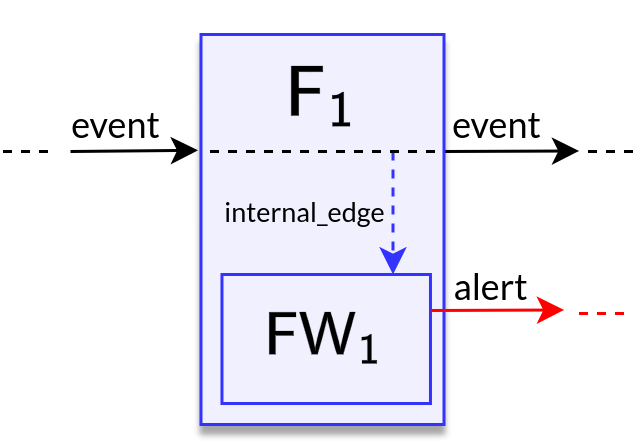
\includegraphics[scale = 1.2]{images/3-Engine/filter-worker.png}
      \caption{Filter Worker detail}
      \label{img:pipeline-schema}
    \end{figure}

    \item \textbf{Multiple Cards Support}\\
    In an initial first toy implementation, we were tracking the activity of only one card per \filter, meaning that for each bank card we were dedicating a \texttt{goroutine} on the form of a \filter stage. This was done as a way to get started, it fast became obvious that this is was an unnecessary waste of computational resources. On a real case scenario, where the number of ATM-card interactions a bank card in a day is not expected to be higher than one on average \fmc{TODO: Poner una referencia formal}, it became clear the need of allowing to share each \filter stage for multiple bank cards.\\

    Formally, as described on \ref{ContinuousQueryEngine}, each \filter \F was implemented to be able to hold a certain subset of root parameters $V_{\mathsf{F}} = \{v_1,\ldots,v_k\}$, representing the Cards being tracked by \F.\\

    In \texttt{Go} to achieve the support of multiple cards per \filter we decided to use hash tables. Go provides a built-in \texttt{map} type that implements a hash table\footnote{\url{https://go.dev/blog/maps}}. We used two different maps, using the card id of the interaction edge $\mathsf{e}$.\emph{number\_id} as the key of both maps.

    \begin{itemize}
        \item \texttt{cardList} \texttt{map}: It is used by \F to determine whether an interaction edge $\mathsf{e}$ belongs to \F, $\mathsf{e} \in$ \F. Only accessed by \F.
        \item \texttt{cardSubgraph} \texttt{map}: To index the interaction edge $\mathsf{e}$ to the corresponding card subgraph.
        Only accessed by \FW. Note that, for our proof of concept, as we are considering only one fraud pattern, we only need one \texttt{cardSubgraph} \texttt{map} data structure. However, note that more will be needed if we consider more fraud patterns with different card subgraphs.
    \end{itemize}

    \begin{center}
    \lstset{style=golangStyle}
    \begin{lstlisting}[caption={Hash Tables \texttt{map} Data Structures on a \emph{Filter} \F stage}]
    var cardList map[string]bool = make(map[string]bool)
    var cardSubgraph map[string]*cmn.Graph = make(map[string]*cmn.Graph)
    \end{lstlisting}
    \end{center}

    % Reason why two maps and not only one
    One could think of using one single \texttt{map} data structure to do the check $\mathsf{e} \in$ \F and at the same time index $\mathsf{e}$ to the corresponding card subgraph, if it is the case. However, the reason why we need two \texttt{maps} and not only one is to respect the architecture of the decoupled event handling. On it, we have two \texttt{goroutines} \F and \FW (as an anonymous internal \texttt{goroutine} of \F) dedicated to check $\mathsf{e} \in$ \F and to do the processing of $\mathsf{e}$, respectively. Having only one \texttt{map} data structure, would mean that both \F and \FW would be doing simultaneous read/write operations on the \texttt{map}, which is unsafe as is not defined what happens (possible race conditions) in \texttt{Go} in this situation. The runtime also warned us to avoid this by alerting us with a fatal error message if we try to share this data structure without any kind of synchronization tool: \textit{\textcolor{red}{Issue: "fatal error: concurrent map read and map write"}}. Therefore a \textit{mutex} or a concurrent map implementation like a \texttt{syncmap} would be needed to control the concurrent access to this shared data structure. For simplicity we decided to avoid sharing the data structure and dedicating one \texttt{map} for each of the \F and \FW stages.

    \item \textbf{Continuous query evaluation}\\
    % Explain the checkFraudI function
    % Fraud pattern 1: obtainTmin -> how this is achieved by retrieving the info from the Neo4j gdb...
    % Fraud patter 0 - tx overlapping -> consider it part of the same?
    As already mentioned, the continuous query evaluation of the different fraud patterns for the cards is accomplished in the \filter stage. For a card $\mathsf{c}$ this is achieved with the evaluation of the algorithms that characterize each of the defined fraud patterns. These algorithms are evaluated over the corresponding card subgraphs and the information retrieved from the stable PG bank database, identifying if there is a subgraph that matches the given patterns and satisfies its constraints.\\
    
    So far, we implemented the fraud pattern I, related with the characterization of a card cloning scenario, as defined in the algorithmic description \ref{alg:check-fraud-def}. 
    In \ref{alg:check-fraud-impl} we provide a more detailed description of the implementation of this algorithm. Whenever a \texttt{EdgeStart} event arrives to \FW through the \internaledgech channel the checking algorithm \texttt{checkFraud} is performed. \texttt{checkFraud} is executed over a non-empty card subgraph $\mathsf{S_c}$ and the interaction \texttt{Edge} $\mathsf{e_{new}}$ of the \texttt{EdgeStart} event. It is checked that there exists a sufficient time distance between $\mathsf{e_{new}}$ and $\mathsf{e_{last}}$; the previous added edge to $\mathsf{Sc}$ before $\mathsf{e_{new}}$.\\
    
    To do it, we need to obtain the minimum needed time \texttt{t\_min} to traverse the distance between the ATMs of the $\mathsf{e_{new}}$ and $\mathsf{e_{last}}$ interactions: $\mathsf{ATM_{last}}$ and $\mathsf{ATM_{new}}$, corresponding to the ATMs with identifiers $\mathsf{e_{last}}.\texttt{ATM\_id}$ and $\mathsf{e_{new}}.\texttt{ATM\_id}$, respectively. \texttt{t\_min} is obtained through the function call $\text{obtainTmin}(\mathsf{e_{last}}, \mathsf{e_{new}})$ on line \ref{line:obtainTmin}. This function obtains the location coordinates of the two ATMs through two \texttt{Cypher} query to the Neo4j stable bank database, using the \texttt{ATM\_id} identifiers (see code listing \ref{lst:cypherQueryCoords}). This is needed since, by definition interaction edges do not contain this information, and therefore the stable bank database needs to be queried to retrieve it, so to be able to do the check of this graph pattern. This query is executed using the function \texttt{ReadQuery} from the \texttt{internal/connection} module of our \DPATM implementation.

    \begin{algorithm}[H]
      \small
      \begin{algorithmic}[1]
      \REQUIRE $\mathsf{S_c}$ is a non-empty subgraph of interaction edges of card $\mathsf{c}$, $\mathsf{e_{new}}$ is the \texttt{Edge} related with the new incoming opening interaction \texttt{EdgeStart} of card $\mathsf{c}$
      \STATE $\mathsf{e_{last}} \gets S_c[|S_c| - 1]$ \COMMENT{Retrieve the last edge from the subgraph $\mathsf{S_c}$}
      \IF{$\mathsf{e_{last}}.\texttt{Tx\_end}$ is empty}
          \STATE \texttt{LOG: Warning: A tx ($\mathsf{e_{new}}$) starts before the previous ($\mathsf{e_{last}}$) ends!} 
          \RETURN
      \ENDIF
      \IF{$\mathsf{e_{last}}.\texttt{ATM\_id} \neq \mathsf{e_{new}}.\texttt{ATM\_id}$}
          \STATE $\texttt{t\_min} \gets \text{obtainTmin}(\mathsf{e_{last}}, \mathsf{e_{new}})$\label{line:obtainTmin}
          \STATE $\texttt{t\_diff} \gets \mathsf{e_{new}}.\texttt{Tx\_start} - \mathsf{e_{last}}.\texttt{Tx\_end}$
          \IF{$\texttt{t\_diff} < \texttt{t\_min}$}   
            \STATE $\text{emitAlert}(\mathsf{e_{last}}, \mathsf{e_{new}})$\label{line:emitAlert}
          \ENDIF
      \ENDIF
      \end{algorithmic}
      \caption{\texttt{checkFraud}($\mathsf{S_c, e_{new}}$)}
      \label{alg:check-fraud-impl}
    \end{algorithm}

    
    \begin{center}
    \lstset{style=cypherStyle}
    \begin{lstlisting}[caption={Code of the constructed \texttt{Cypher} query in \texttt{Go} to obtain the location coordinates of an ATM with its id on the Neo4j graph database}, label={lst:cypherQueryCoords}]
    getATMLocationQuery := 
    MATCH (a:ATM) WHERE a.ATM_id = $ATM_id RETURN 
    a.loc_latitude AS loc_latitude, 
    a.loc_longitude AS loc_longitude
    \end{lstlisting}
    \end{center}

    Once the location coordinates of both ATMs are obtained from the query:
    \begin{itemize}
        \item  $\mathsf{coords_{last}} = (\mathsf{ATM_{last}}.\texttt{loc\_latitude}, \mathsf{ATM_{last}}.\texttt{loc\_logitude})$ 
        \item  $\mathsf{coords_{new}} = (\mathsf{ATM_{new}}.\texttt{loc\_latitude}, \mathsf{ATM_{new}}.\texttt{loc\_logitude})$
    \end{itemize}
    
    then \texttt{t\_min} is calculated as: $\texttt{t\_min} = \texttt{distance}(\mathsf{coords_{last}}, \mathsf{coords_{new}})/\ \texttt{maxSpeed}$.\\
    $\texttt{distance}(\mathsf{coords_{last}}, \mathsf{coords_{new}})$ is the great-circle distance or orthodromic distance between the two coordinate points. It is calculated using the \texttt{Go} haversine package\footnote{\url{https://github.com/umahmood/haversine}}.
    
    \texttt{maxSpeed} is a parametrizable constant indicating the maximum speed at which it is assumed that the distance between any two geographical points can be traveled. So far we defined it to be \texttt{maxSpeed} = 500 km/h. This parameter will have to be defined by the bank system. Of course, a more refined version could calculate this minimum time considering more variables, so to provide a more precise calculation.

    If the required conditions hold, then an \texttt{Alert} is emitted through the \alertch channel to the \sink stage. This is summarized on the function $\text{emitAlert}(\mathsf{e_{last}}, \mathsf{e_{new}})$ on line \ref{line:emitAlert}. The \texttt{Alert} will contain the subgraph built with the two interaction edges causing the alert: $\mathsf{e_{new}}$ and $\mathsf{e_{last}}$ on the \texttt{Subgraph} field, as well as the indication on the type of fraud on its \texttt{Label} field as the type "1" and some optional additional information related with the anomaly on \texttt{Info}. A possible implementation of this function is shown in \texttt{Go} in the \ref{lst:emitAlertImpl} code listing. Note that $\mathsf{out\_alert}$ refers to the output \alertch channel that connects the \filter stage with the \sink stage ( \texttt{chan<- cmn.Alert}).

    \begin{center}
    \lstset{style=golangStyle}
    \begin{lstlisting}[caption={Possible implementation of $\text{emitAlert}(\mathsf{e_{last}}, \mathsf{e_{new}})$}, label={lst:emitAlertImpl}]
            var fraudAlert Alert 
            subgraph := NewGraph()
            subgraph.AddEdge(last_e)
            subgraph.AddEdge(new_e)
            fraudAlert.Label = "1"
            fraudAlert.Info = "fraud pattern"
            fraudAlert.Subgraph = *subgraph
            ...
            out_alert <- fraudAlert
    \end{lstlisting}
    \end{center}
\end{itemize}

With all these ingredients a final \texttt{Go} implementation of the \filter is provided on the code listing \ref{lst:filterImplementation}.

\newpage
\begin{center}
\lstset{style=golangStyle}
\begin{lstlisting}[caption={A \filter stage \texttt{Go} implementation}, label={lst:filterImplementation}]
func filter(event cmn.Event, in_event <-chan cmn.Event, out_event chan<- cmn.Event, out_alert chan<- cmn.Alert) {

var edge cmn.Edge = event.E
var cardList map[string]bool = make(map[string]bool)
var cardSubgraph map[string]*cmn.Graph = make(map[string]*cmn.Graph)
cardList[edge.Number_id] = true
internal_edge := make(chan cmn.Event, cmn.ChannelSize)
// termination synchronization channel F-FW
endchan := make(chan struct{}) 

context := context.Background() 
session := connection.CreateSession(context)
defer connection.CloseSession(context, session)

// FW 
go func() {
 // auxiliary subgraph variable
 var subgraph *cmn.Graph 
 cardSubgraph[edge.Number_id] = cmn.NewGraph()
 subgraph, _ := cardSubgraph[edge.Number_id]
 subgraph.AddEdge(edge)
Worker_Loop:
 for {
    event_worker, _ := <-internal_edge
    switch event_worker.Type {
      case cmn.EOF:
      // finish the worker
      endchan <- struct{}{}
      break Worker_Loop
    case cmn.EdgeStart:
      subgraph, ok = cardSubgraph[event_worker.E.Number_id]
      if !ok {
        // first edge related to the card on subgraph
        cardSubgraph[event_worker.E.Number_id] = cmn.NewGraph()
        subgraph, _ = cardSubgraph[event_worker.E.Number_id]
        subgraph.AddEdge(event_worker.E)
      } else {
        // already an edge of the card
        isFraud, alert := subgraph.CheckFraud(context, session, event_worker.E)
        if isFraud {
          alert.LastEventTimestamp = event_worker.Timestamp
          out_alert <- alert
        }
        // set as new head of the subgraph (only save the last edge)
        subgraph.NewHead(event_worker.E)
      }
    case cmn.EdgeEnd:
      subgraph, ok = cardSubgraph[event_worker.E.Number_id]
        if !ok {
          cardSubgraph[event_worker.E.Number_id] = cmn.NewGraph()
          subgraph, _ = cardSubgraph[event_worker.E.Number_id]
          subgraph.AddEdge(event_worker.E)
        } else {
          subgraph.CompleteEdge(event_worker.E)
        }
    }
    }
}()

// Filter
Filter_Loop:
 for {
    event, _ := <-in_event
    switch event.Type {
    case cmn.EOF:
        internal_edge <- event
        <-endchan
        out_event <- event 
        break Filter_Loop
    case cmn.EdgeStart, cmn.EdgeEnd:
        if cardList[event.E.Number_id] {
            internal_edge <- event
        } else if len(cardList) < cmn.MaxFilterSize {
            cardList[event.E.Number_id] = true
            internal_edge <- event
        } else {
            out_event <- event
        }
    }
}
close(internal_edge)
close(out_event)
}
\end{lstlisting}
\end{center}

% - Generator: Descripción. Código concreto?
\paragraph*{Generator\\}

The \generator \G main functionality is spawning a new \filter \F stage whenever it receives an interaction \texttt{Edge} event. This event is provided as a parameter to the new spawned \F so that it can be then processed there.

Whenever the new \F is spawned, the pipeline is reconnected accordingly: \F takes as \eventch input channel the original \eventch input channel of \G, and \G generates a new \eventch input channel which is set up as the output \eventch channel for \F and as the new input \eventch channel for \G. The \alertch is also provided to \F so that it can utilize as an output channel to send alerts to the \sink stage.

\fmc{Poner extracto código para enseñar mejor?}

% - Sink...
\paragraph*{Sink\\}

The \sink \Sk stage is in charge of reading from the \eventch and \alertch. Its main functionality is to receive the \texttt{alerts} coming from the \alertch and post-processing them accordingly to the bank requirements. In our case, we just write them into an output file to record them. In addition we also maintain a log event output file with the received events received from the \eventch channel.

\fmc{Actualizar los dibujos correspondientes. Poner estos y otros similares a los de la presentación del AMW2024 pero actualizados a este formato.}
\begin{figure}[H]
  \centering
  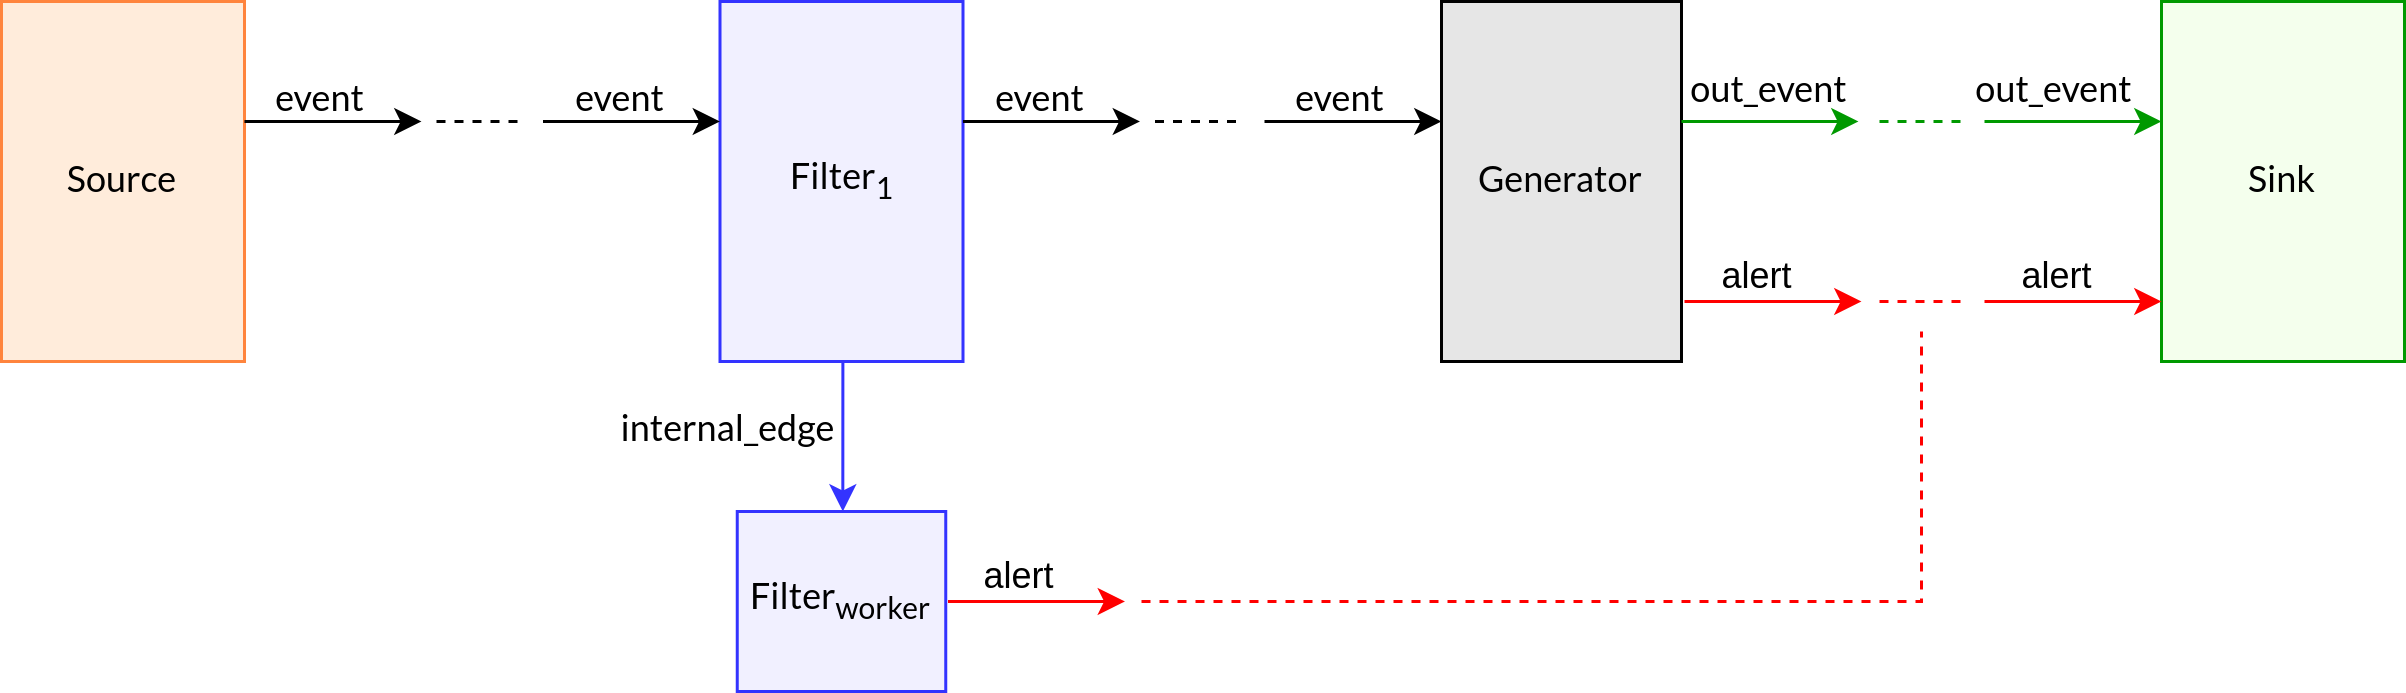
\includegraphics[scale = 0.7]{images/3-Engine/pipeline-schema-filter-detail-old.png}
  \caption{Pipeline Schema with Filter detail}
  \label{img:pipeline-schema-0}
\end{figure}

\begin{figure}[H]
  \centering
  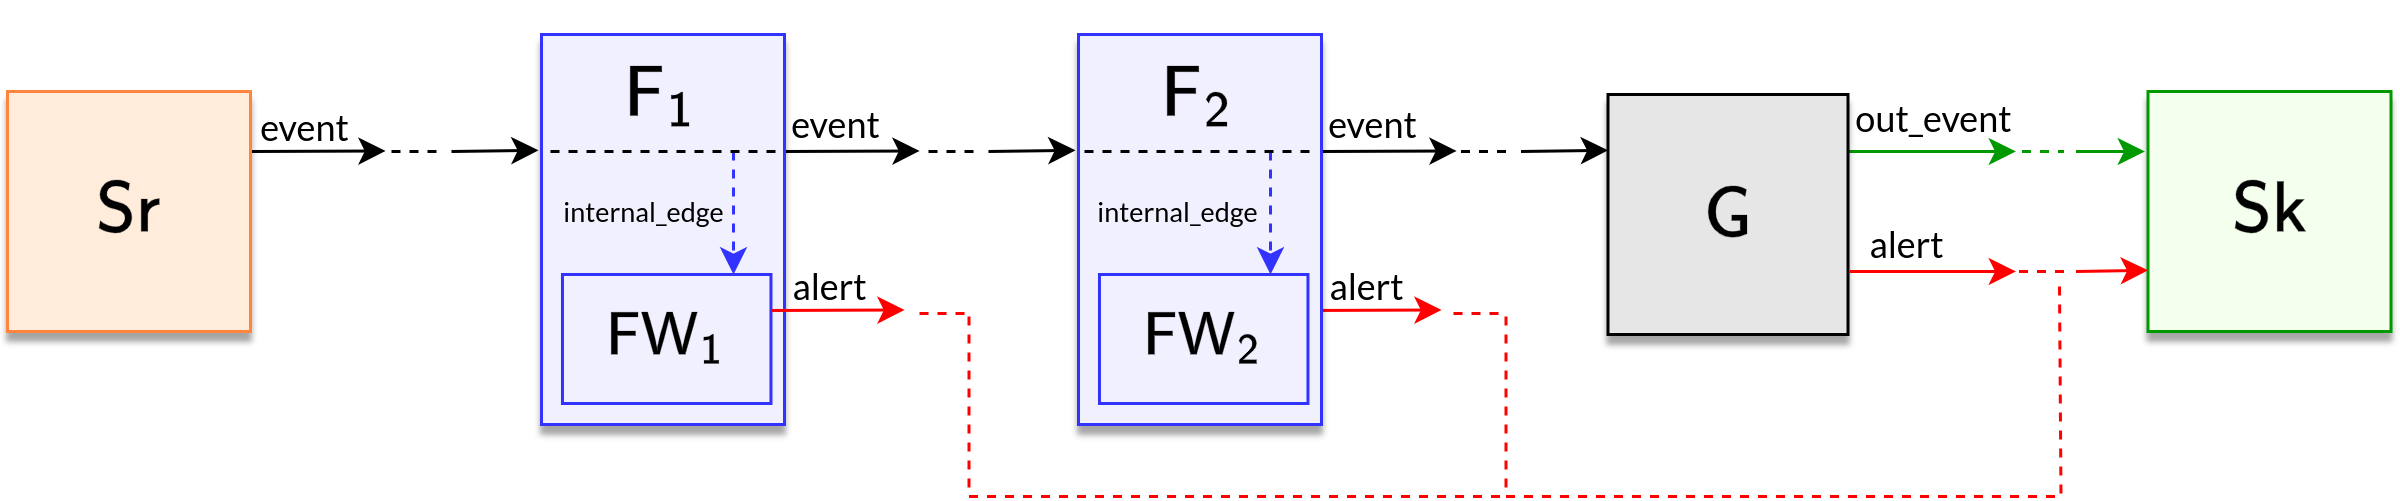
\includegraphics[scale = 0.7]{images/3-Engine/pipeline-schema-filter-detail-1.png}
  \caption{Pipeline Schema with Filter detail 1}
  \label{img:pipeline-schema-1}
\end{figure}

\documentclass{article}
\usepackage[utf8]{inputenc}
\usepackage{graphicx} % Required for inserting images
\usepackage{hyperref}
\usepackage{subcaption}
\usepackage{float}
\usepackage{tcolorbox}
\usepackage{amsmath}
\usepackage{amssymb}
\usepackage{listings}% http://ctan.org/pkg/listings}
\usepackage{algorithm}
\usepackage{algorithmic}
\usepackage[toc,page]{appendix}
%\usepackage[backend=biber]{biblatex}
\usepackage{multicol}
\usepackage{siunitx}
\usepackage{comment}
\usepackage{xcolor}
\usepackage{caption}
\usepackage{forest}
\usepackage{tikz}
\usetikzlibrary{shapes.geometric, arrows}


\tikzstyle{startstop} = [rectangle, rounded corners, 
minimum width=3cm, 
minimum height=1cm,
text centered, 
draw=black, 
fill=red!30]

\tikzstyle{io} = [trapezium, 
trapezium stretches=true, % A later addition
trapezium left angle=70, 
trapezium right angle=110, 
minimum width=3cm, 
minimum height=1cm, text centered, 
draw=black, fill=blue!30]

\tikzstyle{process} = [rectangle, 
minimum width=3cm, 
minimum height=1cm, 
text centered, 
text width=3cm, 
draw=black, 
fill=orange!30]

\tikzstyle{decision} = [diamond, 
minimum width=3cm, 
minimum height=1cm, 
text centered, 
draw=black, 
fill=green!30]
\tikzstyle{arrow} = [thick,->,>=stealth]


\title{TFM-FernandoMartín}
\author{Fernando Martín Canfrán}

\begin{document}
\section{Experiments}

Note that, since the way we did the transaction generator (coming from wisabi database client's behavior), the average number of transactions per day per card is $\sim1$, and therefore to be able to generate a transaction set with anomalous situations more close to reality, a reasonable size for the generated transaction stream would be having $t$ around some weeks or month(s).

\subsection{1st option: Real time-event stream simulation}

Since we do not have the material time to run each experiment for a time $t$ of some weeks or a month the idea is to do time scaling of the time event stream.

Take the stream of a certain time interval size $t$ and map it into a smaller time interval
$t'$ where $t' << t$ so that:
\begin{itemize}
  \item \textbf{Shorter experimental time}: Reduced time to test the system behavior. Instead of $t$, only $t'$ time to test it. 
  \item \textbf{Stress testing}: We do not test the system under a real-case scenario considering its number of cards $c$, instead we are testing it under a higher load to what it would correspond, but having $c$ cards, and therefore $c$ filter's subgraph.
  \item \textbf{Graph database size VS amount of filters' subgraphs}: Although we simulate a higher load, the number of filters' subgraph corresponds to $c$ the number of cards. The benefit is that we do not need to have such a big graph database.
\end{itemize}

The consequences for the experiments and metrics:

\begin{itemize}
  \item \textbf{Diefficiency metrics} (continuous delivery of results): If we give the input stream to the system respecting the temporal timestamps, note that no matter the system characteristics, that a result (an alert in our case), will not be possible to be produced until the event causing it arrives to the system. Therefore the emission of events is expected to be really similar in this case, for any system variation. Only in the case when the stream load is high enough we expect to see some differences??
  \item \textbf{Response time}: having in mind the previous considerations, we think in measuring the possible differences of behavior of the different system capabilities in terms of the mean response time. The mean response time (\texttt{mrt}) would be the average time that the system spends since it receives the transactions involved in an alert until the time it emits the alert.
\end{itemize}

\textcolor{red}{Problems derived to pay attention to}:
\begin{itemize}
  \item Shrinking the timestamps to a smaller time interval, produces the emergence of not real fraud patterns that before did not exist due to their real and "correct" larger time distance. $\rightarrow$ a solution for this is to conserve the original timestamps, and consider the mapped-shrunk-reduced timestamps for simulating the arrival times of the transactions into the system while taking the original timestamps for the checking of the frauds.
\end{itemize}

\subsection{2nd option: real timestamp omission}

Do not consider the real-time simulation, by omitting the transaction timestamps in the sense that we do not consider them to simulate a real case scenario where each transaction arrives to the system at the time indicated by its timestamp. 
Instead all the stream comes (ordered by timestamp) but directly (almost) at the same time to the system. With this approach:
\begin{itemize}
  \item \textbf{No real case simulation}
  \item \textbf{Measure the load the system can take}: for the different system variations given a same stream.
  \item \textbf{Diefficiency metrics}: since time arrival of the transactions to the system is now ignored, and all the transactions come one after the other, a result to be produced do not need to wait for the real timestamp of the transaction. Therefore, we could see the differences in continuously delivering results of the different systems under the same input stream load (more clear than before).
\end{itemize}

Some (other) references:

\begin{itemize}
  \item \href{https://www.confluent.io/es-es/learn/apache-flink/}{Apache Flink}: distributed processing engine for stateful computation of data streams.
\end{itemize}

%\bibliographystyle{plain} % Choose a style (plain, abbrv, unsrt, etc.)
%\bibliography{references} % This points to references.bib  

\end{document}
\newpage
\section{Analysis of Experimental Results}
\label {sec:results}

In what follows we introduce the following notation to refer to the different experiments performed. Let $\Sigma= (g, s(k, p), f, c)$ represent the execution of an experiment where:
\begin{itemize}
    \item $g$ is a datagraph;
    \item $s(k,p)$ represents a stream of transactions of length $k$ and percentage $p$ of anomalous transactions;
    \item $f$ is the number of filters;
    \item $c$ is the number of cores.
\end{itemize}

We perform experiments for: 
\begin{itemize}
    \item $g = $ \smallG\ and \mediumG;
    \item $s(k,p)$: 
    \begin{itemize}
        \item With $g = $ \smallG\ for $k=30, 60, 120$ and $p=0.02$.
        \item With $g = $ \mediumG\ for $k=7, 15$ and $p=0.03$.
    \end{itemize}
    \item $f$: 
    \begin{itemize}
        \item With $g = $ \smallG\ for $f=1,2,5,10,20,40,100,200,500,1000,2000$.
        \item With $g = $ \mediumG\ for $f=1,5,10,100,250,500,1000,2000,5000,10000$.
    \end{itemize} 
    \item $c = 1, 2, 4, 8, 16$
\end{itemize}

For instance, $\Sigma(\mathsf{GDB_A}, s(30, 0.02), f, c)$ refers to the experiment performed with $g = $ \smallG, $k=30$ days stream length and $p=0.02$ anomalous ratio, performed for all the filters $f$ combinations possible for $g = $ \smallG, and for all cores $c$ combinations.\\

\subsection*{E1: Evaluation in a High-Load Stress Scenario}

% Introducción
The evaluation of the \DPATM\ in this scenario was done for the two different bank databases; \smallG\ and \mediumG. 
For each simulated bank database system we provided the transactions streams that we generated. T
he details on the generated datasets are explained on \ref{exps:considered-datasets}. 
Let the Tables \ref{table:bank-dbs-details-again} and \ref{table:stream-sizes-again} serve as a summary.

\begin{table}[H]
\centering
\begin{tabular}{|c|c|c|c|c|}
\hline
\textbf{Name} & \textbf{$|\text{Card}|$} & \textbf{$|\text{ATM}|$} & \textbf{$|\text{ATM}_{\text{Internal}}|$} & \textbf{$|\text{ATM}_{\text{External}}|$} \\ \hline
\smallG    & 2000      & 50     & 40        & 10        \\ \hline
\mediumG    & 500000      & 1000     & 900        & 100        \\ \hline
\end{tabular}
\caption{Bank databases characteristics}
\label{table:bank-dbs-details-again}
\end{table}

\begin{table}[H]
    \small 
    \hspace*{-1.2cm}
    \centering
    \begin{tabular}{|l|c|c|c|c|c|c|}
    \hline
    \textbf{Name} & \textbf{Bank DB} & \textbf{$|\text{Days}|$} & \begin{tabular}[c]{@{}c@{}}\textbf{Anomalous}\\ \textbf{Ratio}\end{tabular} & \textbf{Stream Size} & \textbf{$|\text{Regular Tx}|$} & \textbf{$|\text{Anomalous Tx}|$} \\ \hline
    $\mathsf{GDB_A\text{-}30}$ & \smallG    & 30       & $0.02\ (2\%)$   & 39959       & 39508      & 451   \\ \hline
    $\mathsf{GDB_A\text{-}60}$ & \smallG     & 60       & $0.02\ (2\%)$   & 80744       & 79005      & 1739         \\ \hline
    $\mathsf{GDB_A\text{-}120}$ & \smallG     & 120      & $0.02\ (2\%)$   & 160750      & 157756     & 2994         \\ \hline
    $\mathsf{GDB_B\text{-}7}$ & \mediumG    & 7        & $0.03\ (3\%)$   & 2428286     & 2401806    & 26480        \\ \hline
    $\mathsf{GDB_B\text{-}15}$ & \mediumG    & 15       & $0.03\ (3\%)$   & 4856573     & 4805920    & 50653        \\ \hline
    \end{tabular}
    \caption{ \label{table:stream-sizes-again}Summary of the different streams generated for each of the bank databases. For each stream, we indicate the time interval (in days) that it simulates, the anomalous ratio, its exact stream size (in the number of transactions), and from it, its number of regular and only anomalous transactions.}
\end{table}

For each bank \DPATM\ system to be tested, we considered different \DPATM\ configurations 
regarding the number of filters with which we construct the \DP\ pipeline. 
This is controlled by setting up the system parameter \emph{maxFilterSize}, which determines the maximum number of cards each \filter\ stage tracks. 
Table \ref{table:exps-filters-variations} represents the different \emph{maxFilterSize} configurations tested for each of the bank systems.\\

Each of these \DPATM\ configurations were run for different resources variations in terms of the dedicated number of cores, 
in particular for $c = $\texttt{1}, \texttt{2}, \texttt{4}, \texttt{8} and \texttt{16} cores. 
For each particular number of cores setting the \DPATM\ configurations were compared against a sequential baseline version of our system (cores = \texttt{1}). 
This sequential version is referred in the following results as both the \textit{sequential/baseline} or as the \texttt{0-filter} version. 
It is a simple program version of the \DPATM\ that executes the same algorithm but without a \DP, that is, only with a main process that process the transactions one after the other tracking the activity of all the cards at once. It also implements the same stream ingestion method as the one referred in \ref{exps-input-reading}. However, it is different from the \DPATM\ with one single \filter\ stage in the sense that, this last contains a proper \filter\ \F\ stage with its respective \filterworker\ \FW\ substage, as well as a \source\ \Sr\ and a \sink\ \Sk\ stage.

\begin{table}[H]
    \renewcommand{\arraystretch}{1.5} % control row height
    \centering
    \begin{minipage}{0.45\textwidth}
        \centering
        \begin{tabular}{|c|c|}
        \hline
        \begin{tabular}[c]{@{}c@{}}\textbf{$|\text{Cards}|$ per \filter }\\ (\emph{maxFilterSize})\end{tabular} & \textbf{$|\text{\emph{Filter}}|$} \\ \hline
        2000   &   1     \\ \hline
        1000   &   2     \\ \hline
        400 &   5     \\ \hline
        200  &   10     \\ \hline
        100 &   20    \\ \hline
        50  &   40    \\ \hline
        20  &   100    \\ \hline
        10  &   200    \\ \hline
        4  &   500    \\ \hline
        2  &   1000    \\ \hline
        1  &   2000    \\ \hline
        \end{tabular}
        \caption*{\smallG}
    \end{minipage}
    \hfill
    \begin{minipage}{0.45\textwidth}
        \centering
        \begin{tabular}{|c|c|}
        \hline
        \begin{tabular}[c]{@{}c@{}}\textbf{$|\text{Cards}|$ per \filter }\\ (\emph{maxFilterSize})\end{tabular} & \textbf{$|\text{\emph{Filter}}|$} \\ \hline
        500000   &   1     \\ \hline
        100000   &   5     \\ \hline
        50000 &   10     \\ \hline
        5000  &   100     \\ \hline
        2000 &   250    \\ \hline
        1000  &   500    \\ \hline
        500  &   1000    \\ \hline
        250  &   2000    \\ \hline
        100  &   5000    \\ \hline
        50  &   10000    \\ \hline
        10  &   50000    \\ \hline
        \end{tabular}
        \caption*{\mediumG}
    \end{minipage}
    \caption{For \smallG\  and \mediumG, the different \DPATM\ configurations combinations for the \emph{maxFilterSize} parameter, including the derived number of \filter\ stages of the \DPATM.}
    \label{table:exps-filters-variations}
\end{table}

Each job was run ten times in the case of the experiments of the \smallG\ and one in the case of the \mediumG\ experiments, due to time constraints and its longer execution times. We limited to \texttt{16}GB of RAM the amount of memory used for each experiment. Note that in the case of the \mediumG, the tests with 50000 filters could not be performed due to this memory limitation.

% 1. Is it worthy the DPATM
\subsubsection*{\DPATM\ Comparison to Sequential Baseline}

First we provide and study the results to compare our different \DPATM\ configurations (with the different number of filters variations) with respect to the sequential version of the program, the \texttt{0-filter} version.\\

In Figure \ref{img:exps-small-120-combined} we can see the comparison of different metrics results for the experiment $\Sigma(\mathsf{GDB_A}, s(120, 0.02), f, c)$. We can see that the performance of the sequential version is, in general, the worst regarding all the metrics except for the Mean Response Time (\texttt{MRT}), where the \texttt{0-filter} exhibits a lower \texttt{MRT} than many configurations of the \DPATM, no matter the number of cores (\ref{fig:exps-small-120-mrt}).\\

In this sense, the sequential version achieves a lower \texttt{MRT} for any configuration with a number of filters above 40. Only the variations with a number of filters in the range 5-20 are able to outperform the sequential version on this metric, showing a \texttt{MRT} around 5-6 seconds in the 5 and 10 filter cases, for all the number of cores tested. To get more insights on this, we show in Figure \ref{img:exps-small-120-traces-reduced} the Response Time (\texttt{RT}) trace of the different configurations run with \texttt{16} cores. On it, as mentioned, we can see that only the configurations with a number of filters in the range 5-20 tend to have a \texttt{RT} below the sequential version for all of the checks. The 1-filter version is always above. However, an interesting phenomena that we see is that for the versions with 40 and more filters the \texttt{RT} presents a linear growing shape, whereas for the other versions the \texttt{RT} tends to be constant for all the performed checks. These \textit{large} number of filters versions even present a lower \texttt{RT} up to a certain number of checks. Later we will come again to this discussion, so to analyze better why this could be the cause of this behavior.
\\ 

Nevertheless, as expected, the sequential version underperforms for the other metrics such as the
Execution Time \texttt{ET} (\ref{fig:exps-small-120-et}), the throughput \texttt{T} (\ref{fig:exps-small-120-t}) and the \texttt{dief@t} (\ref{fig:exps-small-120-dieft}). In Figure \ref{img:exps-small-120-radar-dieft} we show the comparison of all these metrics together with a radar plot for the experiment $\Sigma(\mathsf{GDB_A}, s(120, 0.02), f, 16)$. A similar behavior can be observed in the experiments done for \mediumG. In Figure \ref{img:exps-medium-7D-radar-dieft}, we show the radar plot of the $\Sigma(\mathsf{GDB_B}, s(7, 0.03), f, 16)$ experiment. On it, again, only the versions with a number of filters in the range 5-20 outperform the sequential version in the \texttt{MRT}. However, for the rest of the metrics we can observe that, in general, almost all \DPATM\ configuration exhibits a better performance than the sequential version. \\


\begin{figure}[H]
    \centering
    \hspace*{-3cm} % Move content to the left
    \begin{subfigure}{0.5\textwidth}
        \centering
        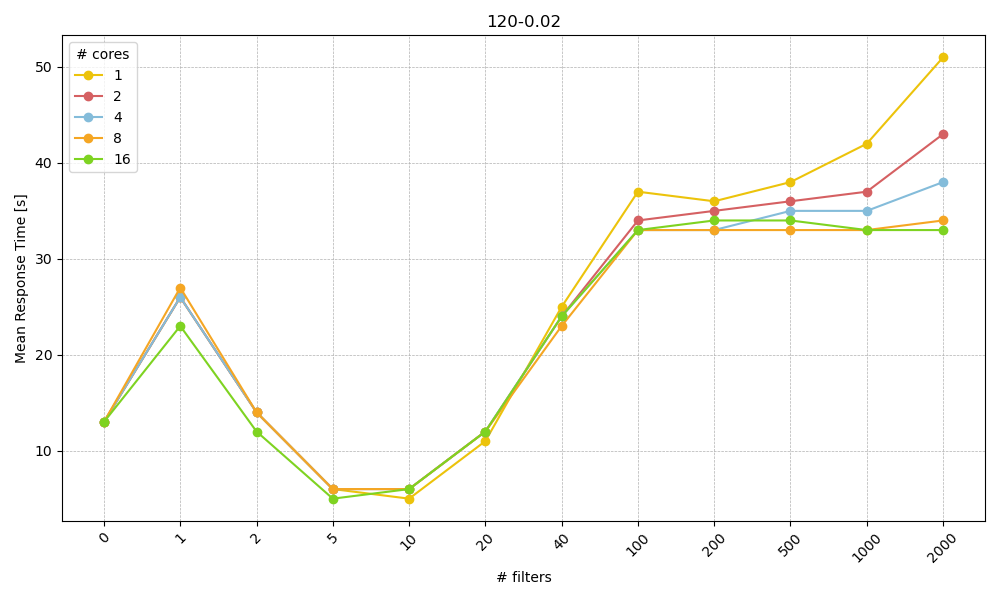
\includegraphics[scale=0.4]{images/4-Experiments/NRT/small/120-0.02/combined/mrt-1.png}
        \caption{Mean Response Time \texttt{MRT} (in seconds)}
        \label{fig:exps-small-120-mrt}
    \end{subfigure}
    \hspace{0.16\textwidth}
    \begin{subfigure}{0.5\textwidth}
        \centering
        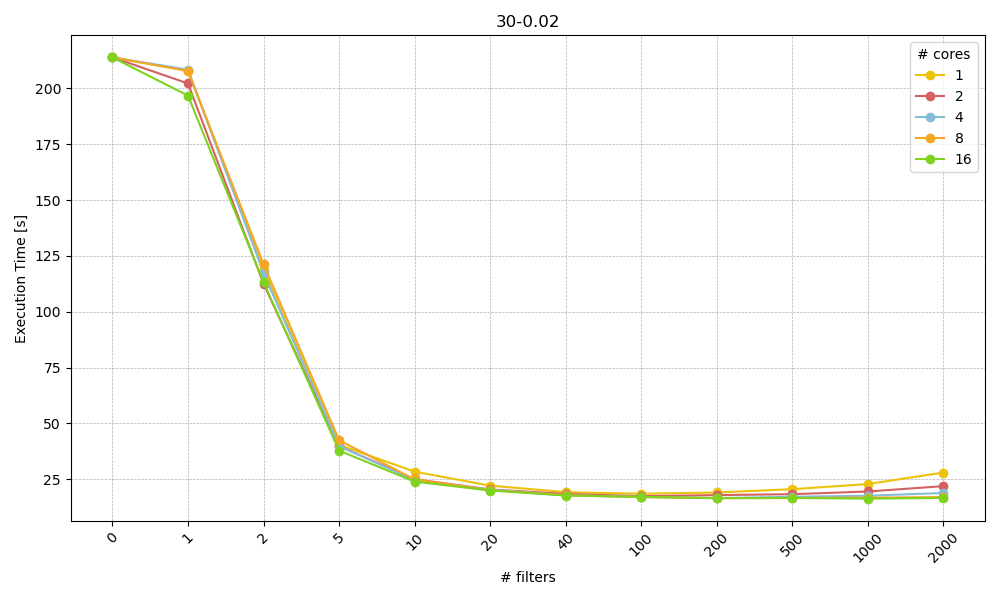
\includegraphics[scale=0.4]{images/4-Experiments/NRT/small/120-0.02/combined/execTime-1.png}
        \caption{Execution Time \texttt{ET} (in seconds)}
        \label{fig:exps-small-120-et}
    \end{subfigure}
    
    \vspace{0.5cm} % Vertical space between rows

    \hspace*{-3cm} % Move content to the left for the second row
    \begin{subfigure}{0.5\textwidth}
        \centering
        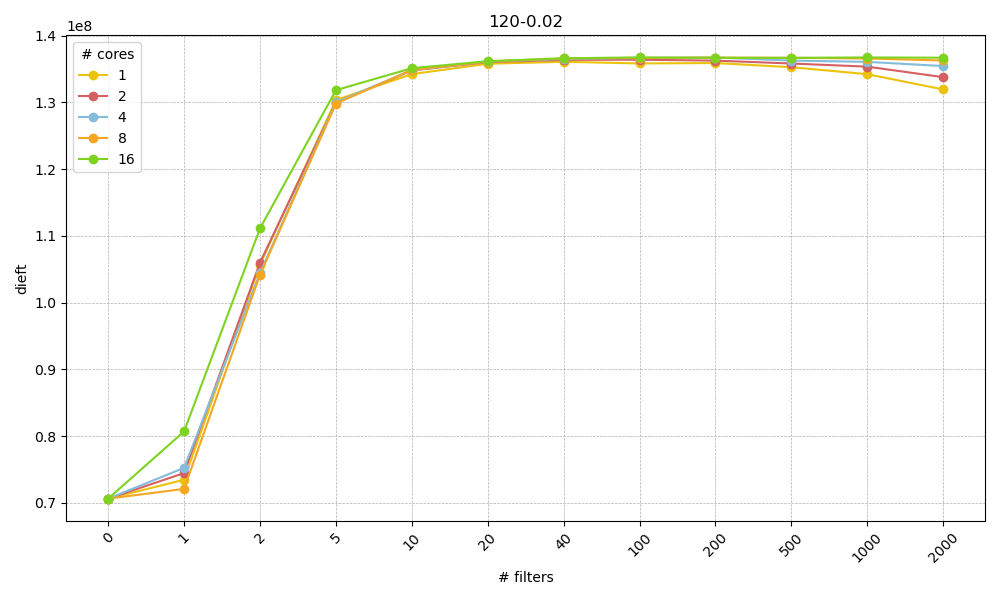
\includegraphics[scale=0.4]{images/4-Experiments/NRT/small/120-0.02/combined/dieft-1.png}
        \caption{\texttt{dief@t}}
        \label{fig:exps-small-120-dieft}
    \end{subfigure}
    \hspace{0.16\textwidth}
    \begin{subfigure}{0.5\textwidth}
        \centering
        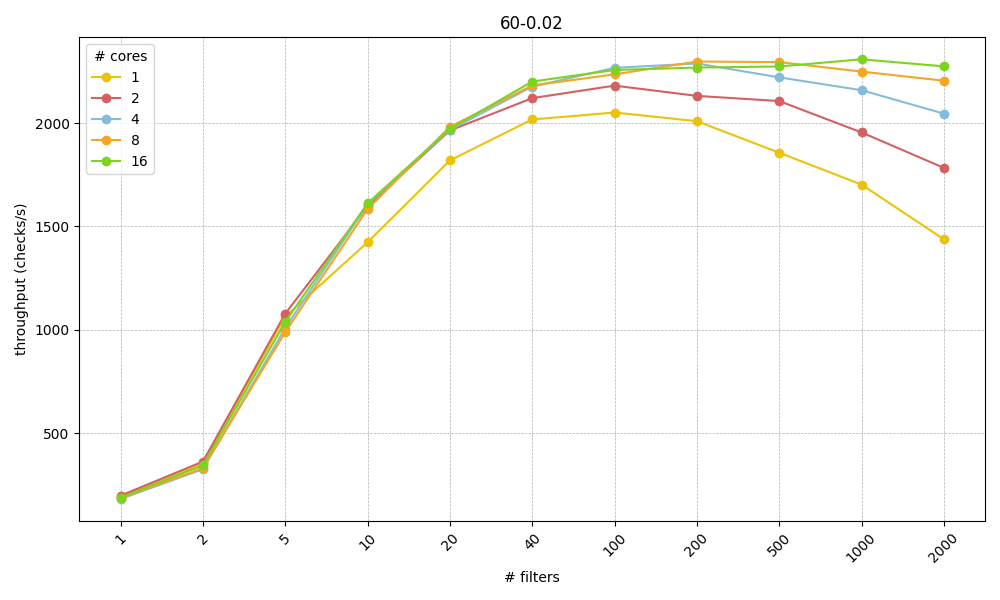
\includegraphics[scale=0.4]{images/4-Experiments/NRT/small/120-0.02/combined/throughput-1.png}
        \caption{Throughput \texttt{T} (checks/s)}
        \label{fig:exps-small-120-t}
    \end{subfigure}

    \caption{Metrics comparison for experiment $\Sigma(\mathsf{GDB_A}, s(120, 0.02), f, c)$. Each color represents the experiment run with a different number of cores.
    (a) \texttt{MRT}, (b) \texttt{ET}, (c) \texttt{dief@t}, (d) \texttt{T}.}
    \label{img:exps-small-120-combined}
\end{figure}

\begin{figure}[H]
    \centering
    \includegraphics[scale=0.6]{images/4-Experiments/NRT/small/120-0.02/fixedcores/16c/traces-response-time-reduced.png}
    \caption{Response Time (\texttt{RT}) trace for the $\Sigma(\mathsf{GDB_A}, s(120, 0.02), f, 16)$ test. Horizontal axis shows the \emph{check} number and the vertical axis shows the \texttt{RT} (in seconds) for that check.}
    \label{img:exps-small-120-traces-reduced}
\end{figure}

\begin{figure}[H]
    \centering
    \includegraphics[scale=0.6]{images/4-Experiments/NRT/small/120-0.02/fixedcores/16c/radar-dieft.png}
    \caption{Metrics radar plot comparison for the $\Sigma(\mathsf{GDB_A}, s(120, 0.02), f, 16)$ experiment. Each axis represents a metric: \texttt{MRT$^{-1}$}, \texttt{T} (Throughput), \texttt{dief@t}, \texttt{TFFT$^{-1}$} and \texttt{ET$^{-1}$}. Better performance for a metric is achieved whenever the value is closer to the outer boundary of the corresponding axis.}
    \label{img:exps-small-120-radar-dieft}
\end{figure}

\begin{figure}[H]
    \centering
    \includegraphics[scale=0.6]{images/4-Experiments/NRT/medium/7-0.03/fixedcores/16c/radar-dieft.png}
    \caption{Metrics radar plot comparison for the $\Sigma(\mathsf{GDB_B}, s(7, 0.03), f, 16)$ experiment. Each axis represents a metric: \texttt{MRT$^{-1}$}, \texttt{T} (Throughput), \texttt{dief@t}, \texttt{TFFT$^{-1}$} and \texttt{ET$^{-1}$}. Better performance for a metric is achieved whenever the value is closer to the outer boundary of the corresponding axis.}
    \label{img:exps-medium-7D-radar-dieft}
\end{figure}

\subsubsection*{Analysis of the Number of Filters Configuration}

Regarding the configuration of the \DPATM\ system, we are interested in analyzing which is the best configuration in terms of the number of filters for each the \smallG\ and \mediumG, given a certain number of cores resource limitation.\\

% smallG 
For \smallG, as already mentioned for the $\Sigma(\mathsf{GDB_A}, s(120, 0.02), f, c)$ test, regarding the \texttt{MRT} the configurations using 5-10 number of filters exhibit the best \texttt{MRT}, of around 5-6 seconds, worsening for the configurations with a large number of filters (see Figure \ref{fig:exps-small-120-mrt}). Indeed they show a constant and low response time in comparison with the ones with large number of filters; see Figure \ref{fig:exps-small-120-et}.\\

Nonetheless, these configurations do not perform that well in the case of the \ET\ or the \dieft, where a larger number of filters seems to be a better option, being able to consume the input stream faster and showing a better continuous behavior in terms of \dieft. However, it is worthy to note that the behavior tends to degrade for all the metrics in the case of having a low number of cores. We can see this clearly for the case of the runs with \texttt{1} core. It can be seen that, in this case, a large number of filters could be causing an overhead and therefore producing this degradation of the behavior for the \ET\ and the \dieft. We can observe this in all the metrics figures of Figure \ref{img:exps-small-120-combined}, where specially for the \texttt{1} core variations, we can appreciate the degradation for the large number of filters configurations (in the rightmost part of each of the plots). As expected, more cores help to improve the behavior, especially for the variants with large number of filters.\\

The analysis on the number of filters configuration is quite similar in the case of the experiments done for \mediumG. For instance, in Figure \ref{img:exps-medium-15D-8c-radar-dieft} we show the metrics radar for $\Sigma(\mathsf{GDB_B}, s(15, 0.03), f, 8)$, where we can also see that the configurations that achieve the best \MRT\ are the ones with a number of filters in the range 5-10, whereas they are the ones that underperform in the \ET\ and \dieft\ metrics. This can also be seen in the results trace of this same test on Figure \ref{img:exps-medium-15D-8c-trace}, where the continuous behavior for these filter configurations underperforms the continuous behavior for configurations with higher number of filters. However, they have a better continuous behavior than the sequential or the 1 filter configurations.\\

\begin{figure}[H]
    \centering
    \includegraphics[scale=0.6]{images/4-Experiments/NRT/medium/15-0.03/fixedcores/8c/radar-dieft.png}
    \caption{Metrics radar plot comparison for $\Sigma(\mathsf{GDB_B}, s(15, 0.03), f, 8)$. Each axis represents a metric: \texttt{MRT$^{-1}$}, \texttt{T} (Throughput), \texttt{dief@t}, \texttt{TFFT$^{-1}$} and \texttt{ET$^{-1}$}. Better performance for a metric is achieved whenever the value is closer to the outer boundary of the corresponding axis.}
    \label{img:exps-medium-15D-8c-radar-dieft}
\end{figure}

\begin{figure}[H]
    \centering
    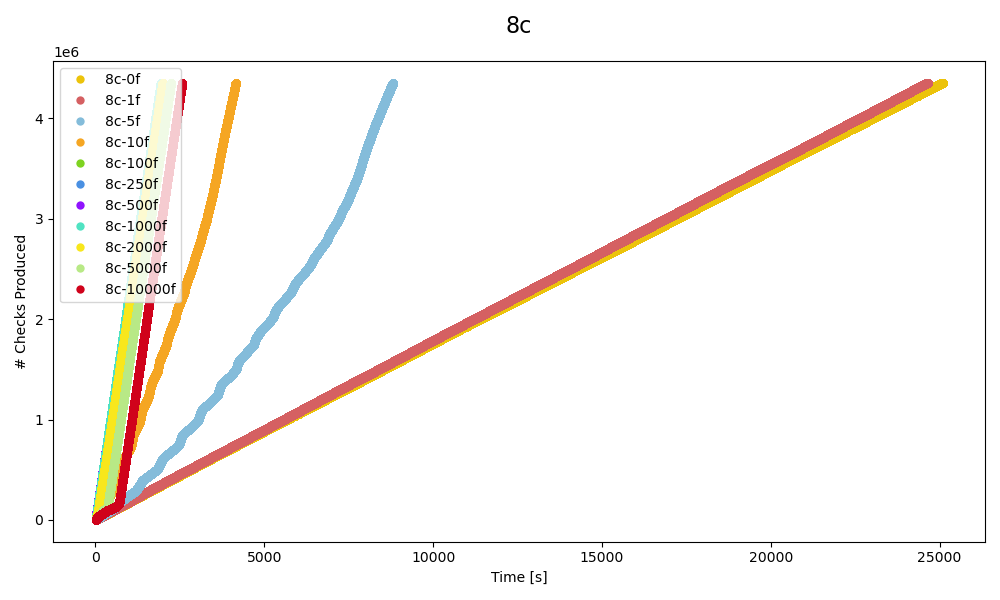
\includegraphics[scale=0.6]{images/4-Experiments/NRT/medium/15-0.03/fixedcores/8c/traces.png}
    \caption{Check results trace for $\Sigma(\mathsf{GDB_B}, s(15, 0.03), f, 8)$. Pairs (result, time(s)). Vertical axis shows the \emph{check} number and horizontal axis shows the time in seconds at which that check is produced.}
    \label{img:exps-medium-15D-8c-trace}
\end{figure}

Another aspect in which the configurations in the range of 5-10 number of filters outperform, apart from achieving the lowest \MRT\ is in achieving it through a constant \RT\ along all the execution. Figure \ref{img:exps-medium-15-rtraces-reduced} shows the response time trace for the $\Sigma(\mathsf{GDB_B}, s(15, 0.03), f, 8)$. On it, the 5-filter variant maintains a \RT\  around 11 seconds and the 10-filter around 9 seconds, in comparison to other larger number of filters variations that end up accumulating more than 100s of \RT.\\

\begin{figure}[H]
    \centering
    \includegraphics[scale=0.6]{images/4-Experiments/NRT/medium/15-0.03/fixedcores/8c/traces-response-time-reduced.png}
    \caption{Response Time (\texttt{RT}) trace for $\Sigma(\mathsf{GDB_B}, s(15, 0.03), f, 8)$. Horizontal axis shows the \emph{check} number and the vertical axis shows the \texttt{RT} (in seconds) for that check.}
    \label{img:exps-medium-15-rtraces-reduced}
\end{figure}

In addition, the degradation of the behavior of the configurations with a high number of filters for a low number of cores executions is a phenomena that we can also see in the \mediumG\ experiments. For instance we can see the degradation of the \ET\ in Figure \ref{img:exps-medium-7-et} in the case of the test $\Sigma(\mathsf{GDB_B}, s(7, 0.03), f, c)$. On it, we observe how the \ET\ deteriorates for the configurations with a high number of filters (2000, 5000 and 10000) whenever we reduce the number of cores. This can be due to: (i) an overhead on the number of \texttt{goroutines} utilized and the overhead in the communication of the pipeline that this might be causing; (ii) the overhead on the communication to the Neo4j graph database instance through those many parallel sessions, remember that we have one parallel session per filter stage; (iii) a bottleneck at the \sink \Sk\ stage, caused by its current file writing of the results. However, note that in a real implementation of the system the results emission would be done in another manner, such as the emission of the alerts through the network to the cardholder. In any case, further investigation and potential improvements to address this issue will be considered as future work.


\begin{figure}[H]
    \centering
    \hspace*{-1.7cm} % Move content to the left
    \begin{subfigure}{0.5\textwidth}
        \centering
        \includegraphics[scale=0.55]{images/4-Experiments/NRT/medium/7-0.03/fixedcores/1c/execTime.png}
        \caption{}
        \label{fig:exps-medium-7-mrt-1c}
    \end{subfigure}
    \hspace*{1cm} 
    \begin{subfigure}{0.5\textwidth}
        \centering
        \includegraphics[scale=0.55]{images/4-Experiments/NRT/medium/7-0.03/fixedcores/2c/execTime.png}
        \caption{}
        \label{fig:exps-medium-7-mrt-4c}
    \end{subfigure}

    \vspace{0.5cm} % Vertical space between rows

    \hspace*{-1.7cm} % Move content to the left for the second row
    \begin{subfigure}{0.5\textwidth}
        \centering
        \includegraphics[scale=0.55]{images/4-Experiments/NRT/medium/7-0.03/fixedcores/4c/execTime.png}
        \caption{}
        \label{fig:exps-medium-7-mrt-8c}
    \end{subfigure}
    \hspace*{1cm}
    \begin{subfigure}{0.5\textwidth}
        \centering
        \includegraphics[scale=0.55]{images/4-Experiments/NRT/medium/7-0.03/fixedcores/8c/execTime.png}
        \caption{}
        \label{fig:exps-medium-7-mrt-16c}
    \end{subfigure}

    \caption{\ET\ for $\Sigma(\mathsf{GDB_B}, s(7, 0.03), f, c)$. (a) Run with $c=$ \texttt{1} core. (b) Run with $c=$ \texttt{2} cores. (c) Run with $c=$ \texttt{4} cores. (d) Run with $c=$ \texttt{8} cores.}
    \label{img:exps-medium-7-et}
\end{figure}

% Enseñar el rt que permanece constante
% Sacar tabla con mrt para cada una de las variantes con 5,10,20f... o algo asi ->
% justificar que el dpatm con esta config es conveniente como real time system en este escenario... etc... HACER COMO UN CIERRE
Finally, since we consider \MRT\ one of the most important metrics for assessing the suitability of our \DPATM\ as a real-time system for the rapid detection of card-ATM fraud, we show Tables \ref{table:mrt-comparison-small-120} and \ref{table:mrt-comparison-medium-15} on which we show the \MRT\ values in seconds for the experiments performed on the \smallG\ and \mediumG\ largest tested streams, $k=120$ and $k=15$, respectively. On them we can show that, in the case of the $\Sigma(\mathsf{GDB_A}, s(120, 0.02), f, c)$ the best filter (5 and 10 filters) configuration has a \MRT\ around 5-6 seconds for all the tested number of cores variation. For the $\Sigma(\mathsf{GDB_B}, s(15, 0.03), f, c)$, the best filter configurations in this metric, again the 5 and 10 filter configurations, achieve a \MRT\ around 10 seconds.

\begin{table}[H]
    \centering
    \begin{tabular}{|c||c|c|c|c|c|}
        \hline
        \multicolumn{6}{|c|}{\textbf{MRT (s) for \smallGOneTwoZero}} \\
        \hline
        \multicolumn{6}{|c|}{Number of Cores} \\
        \hline
        \textbf{\# Filters} & \textbf{1} & \textbf{2} & \textbf{4} & \textbf{8} & \textbf{16} \\
        \hline
        $\mathsf{0}$     & 13  & 13  & 13  & 13  & 13  \\
         $\mathsf{1}$     & 26  & 26  & 26  & 27  & 23  \\
         $\mathsf{2}$     & 14  & 14  & 14  & 14  & 12  \\
         $\mathsf{5}$     & 6   & 6   & 6   & 6   & 5   \\
         $\mathsf{10}$    & 5   & 6   & 6   & 6   & 6   \\
         $\mathsf{20}$    & 11  & 12  & 12  & 12  & 12  \\
        $\mathsf{40}$   & 25  & 24  & 24  & 23  & 24  \\
         $\mathsf{100}$   & 37  & 34  & 33  & 33  & 33  \\
         $\mathsf{200}$   & 36  & 35  & 33  & 33  & 34  \\
        $\mathsf{500}$   & 38  & 36  & 35  & 33  & 34  \\
         $\mathsf{1000}$  & 42  & 37  & 35  & 33  & 33  \\
         $\mathsf{2000}$  & 51  & 43  & 38  & 34  & 33  \\
        \hline
    \end{tabular}
    \caption{Mean Response Time (\MRT) in seconds for the $\Sigma(\mathsf{GDB_A}, s(120, 0.02), f, c)$ experiment.}
    \label{table:mrt-comparison-small-120}
\end{table}


\begin{table}[H]
    \centering
    \begin{tabular}{|c||c|c|c|c|c|}
        \hline
        \multicolumn{6}{|c|}{\textbf{MRT (s) for \mediumGFifteen}} \\
        \hline
        \multicolumn{6}{|c|}{Number of Cores} \\
        \hline
        \textbf{\# Filters} & \textbf{1} & \textbf{2} & \textbf{4} & \textbf{8} & \textbf{16} \\
        \hline
         $\mathsf{0}$     & 13   & 13   & 13   & 13   & 13   \\
         $\mathsf{5}$     & 11   & 10   & 11   & 11   & 9    \\
         $\mathsf{10}$    & 11   & 9    & 10   & 9   & 7    \\
         $\mathsf{100}$   & 33   & 40   & 29   & 23   & 37   \\
         $\mathsf{250}$   & 124  & 80   & 91   & 69   & 90   \\
         $\mathsf{500}$   & 221  & 161  & 134  & 136  & 138  \\
         $\mathsf{1000}$  & 502  & 301  & 267  & 256  & 263  \\
         $\mathsf{2000}$  & 937  & 702  & 618  & 562  & 554  \\
         $\mathsf{5000}$  & 2830 & 1732 & 1422 & 1124 & 1060 \\
         $\mathsf{10000}$ & 4957 & 2535 & 2025 & 1410 & 1249 \\
        \hline
    \end{tabular}
    \caption{Mean Response Time (\MRT) in seconds for the $\Sigma(\mathsf{GDB_B}, s( 15, 0.03), f, c)$ experiment.}
    \label{table:mrt-comparison-medium-15}
\end{table}

% Pongo lo de las interactions per second y su plot
\begin{figure}[H]
    \centering
    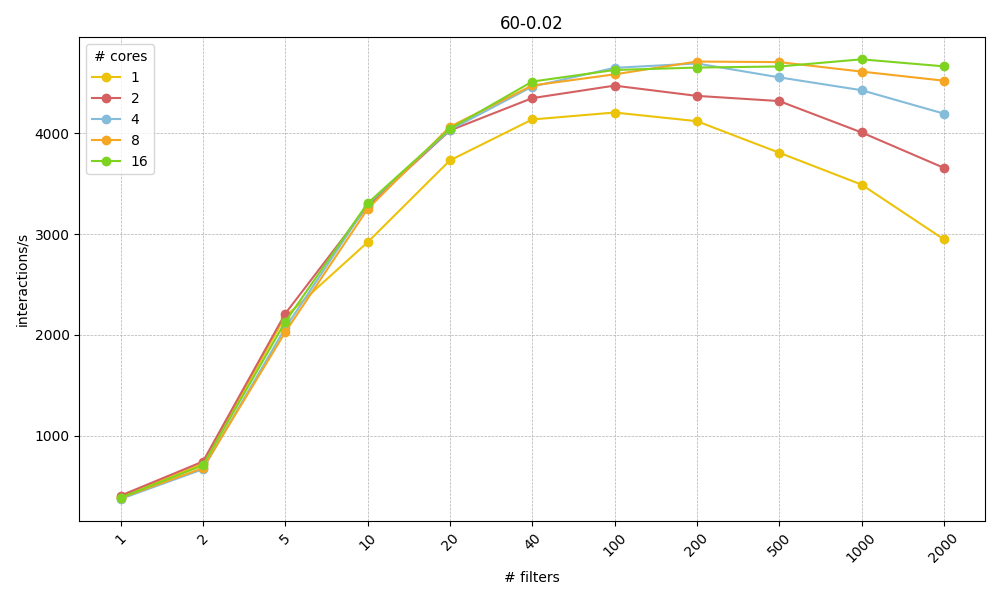
\includegraphics[scale=0.6]{images/4-Experiments/NRT/small/120-0.02/combined/interactions-1.png}
    \caption{Processed \texttt{interactions/s} on the experiment $\Sigma(\mathsf{GDB_A}, s(120, 0.02), f, c)$. Horizontal axis shows the variation in the number of filters $f$. Vertical axis shows the number of processed \texttt{interactions/s}. Each color represents the run with a different number of cores $c$.}
    \label{img:exps-small-120-interactions-new}
\end{figure}

% Mencionar el tradeoff
To sum up, we can say that there is a trade-off between \MRT\ and the other metrics. The \DPATM\ configurations that offer the best balance across all metrics are those with 5 to 10 filters. We reason that this is the case since, as we already discussed in \ref{exps-design-e1}, we consider that a real-time system in this high-load stress scenario needs to show a good performance in various aspects. First, have a low and non-increasing - if possible - response time, so to allow the user / bank system be able to prevent potential the current and future frauds as fast as possible. In this sense, these configurations achieve reasonable low \MRT\ times, in all the cases lower than 11 seconds. Secondly, they also have a reasonable good continuous behavior and have a good performance in terms of the speed to process the stream input. For instance, in $\Sigma(\mathsf{GDB_A}, s(120, 0.02), f, c)$ experiment, we are able to achieve a rate of almost 5,000 \texttt{interactions/s} (2,500 transactions/s) processed (see the Figure \ref{img:exps-small-120-interactions-new}).
Therefore, we conclude that these \DPATM\ configurations achieve a good balance across all these aspects.

\begin{frame}{Conclusions}
\DPATM\ proved to be a effective real-time system with:
\vspace{1em}
\begin{itemize}
    \item \textbf{100\% accuracy}.
    \vspace{1em}
    \item \textbf{Low} and \textbf{constant} response time \texttt{RT} (less than 11s in all cases).
    \vspace{1em}
    \item A stream \textbf{processing capacity speed} that suggest that the \DPATM\ can be extrapolated to \textbf{real big bank systems} ($> 100$M of transactions per day).
\end{itemize}
\vspace{2em}
$\rightarrow$ Working version of \DPATM\ publicly available on Github\footnote{\url{https://github.com/FCanfran/ATM-DP}}

\end{frame}

\begin{frame}{Future Work}
\begin{itemize}
    \item Investigate/\textbf{Improve} the \textbf{response time} performance for the combinations with \textbf{large} number of \textbf{filters}.
    \vspace{0.5em}
    \item Include \textbf{more types} of ATM \textbf{card frauds} or even other kind of frauds (POS or CNP):
    \vspace{0.5em}
        \begin{itemize}
            \item[$\ast$] \emph{Card cloning} characterization
            \item[$\ast$] \emph{Lost-and-stolen} card characterization
            \item[$\circ$] Anomalous location usage
            \item[$\circ$] Anomalous number of operations
            \item[$\circ$] Anomalous high expenses
        \end{itemize}
    \vspace{0.5em}
    \item Study the problem of \textbf{window management}.
    \vspace{0.5em}
    \item Experiment with \textbf{larger} banking data \textbf{graphs}.
\end{itemize}
\vspace{0.3em}
$\rightarrow$ Partial results of this work were reported and presented in the Alberto Mendelzon
Workshop 2024.
\end{frame}




\newpage
\printbibliography 

%\newpage
%\bibliography{ATM}

\end{document}
